%%%%%%%%%%%%%%%%%%%%%%%%%%%%%%%%%%%%%%%%%
% University Assignment Title Page 
% LaTeX Template
% Version 1.0 (27/12/12)
%
% This template has been downloaded from:
% http://www.LaTeXTemplates.com
%
% Original author:
% WikiBooks (http://en.wikibooks.org/wiki/LaTeX/Title_Creation)
%
% License:
% CC BY-NC-SA 3.0 (http://creativecommons.org/licenses/by-nc-sa/3.0/)
% 
% Modified for COSC480/490 by:
% Lech Szymanski (8/3/18)

\documentclass[12pt]{article}
\usepackage[draft]{cosc4x0style}
%\usepackage{cosc4x0style}
\usepackage[T1]{fontenc}
\usepackage{subcaption}
\usepackage{caption}
\usepackage{hyperref}
\usepackage{fvextra}
\usepackage{csquotes} 
\usepackage{biblatex}
\usepackage{listings}
\usepackage{float}
\usepackage{array}
\usepackage{threeparttable}
\usepackage{multirow}
\usepackage{booktabs}
\usepackage{dirtytalk}
\usepackage{xcolor}
\usepackage{soul}
\addbibresource{refs.bib}
\usepackage{listings}
\usepackage{geometry}
% To compile the final version of the report (which will remove all the todo content)

% Specify project code 480 or 490 \papercode{480}

% Your project title
\title{An Exploration of the Common Vulnerability Scoring System}

% Your name
\author{Jake \textsc{Norton}}
\studentid{5695756}

% Names of your supervisors, separated by line break '\\'
\supervisors{
  Dr.\@ David \textsc{Eyers} \\
  Dr.\@ Veronica \textsc{Liesaputra}
}

% Date, change the \today to a set date if you want to be precise
\reportdate{\today}

% Dave's editing macros
\newcommand{\note}[2][red]{\textcolor{#1}{#2}}
\newcommand{\notedme}[1]{\note[blue]{[<Dave> #1]}}
\newenvironment{scaffold}{\color{red}}{}
\newcommand{\change}[2][]{\textcolor{orange}{#2}}

\begin{document}


\maketitle

\begin{abstract}

	The Common Vulnerability Scoring System (CVSS) is designed to produce scores for software
	vulnerabilities, serving as a crucial tool for triaging the increasing number of new
	vulnerabilities released each year. As manual scoring cannot keep pace with this growth,
	\notedme{Claim feels a bit off: it's more that at the moment the trend is rising faster than the employed set of staff to handle the situation.}
	there
	is a need for automated prediction methods. While machine learning, particularly large language
	models (LLMs), have shown promise in predicting CVSS metrics given there descriptions.
	\notedme{This isn't a sentence (preceding) and `their' not `there'.}
	This
	paper aims to explore the CVE and CVSS processes to provide a foundation for future research.
	This paper explores the potential of using multiple data sources for cross-validation and
	increased training data volume, specifically comparing NVD with the MITRE database. The analysis
	reveals differences in how these databases rate Common Vulnerabilities and Exposures (CVEs),
	highlighting the challenges in establishing a consistent ground truth for CVSS scores. While the
	combination of multiple datasets did not yield the expected improvements in prediction accuracy,
	this investigation provides valuable insights into the complexities of CVSS scoring across
	different evaluation teams. The next focus of this paper is on enhancing the interpretability
	and analysis of CVE/CVSS data through clustering techniques and other dataset analysis methods.
	I employ Latent Dirichlet Allocation (LDA) and other clustering approaches to uncover patterns
	within the vulnerability descriptions. The findings demonstrate that certain types of vulnerabilities
	tend to cluster together, such as cross-site scripting, and denial-of-service attacks.
\end{abstract}


\section{Introduction}

In 2023, there were 29,065 new vulnerabilities recorded, as illustrated in Figure~\ref{fig:cves_per_year}.
This number continues to rise year on year, underscoring the growing challenge of managing and
prioritizing software vulnerabilities. These vulnerabilities are documented using the Common
Vulnerabilities and Exposure system (CVE~\cite{CVE}), with CVSS scores derived from these entries to
indicate severity and impact. The National Vulnerability Database (NVD~\cite{NVD}) serves as the
primary source for CVSS-enriched CVE data and is widely used in research (e.g., \cite{costa,
	nvd_example1, nvd_example2}). However, to explore the potential benefits of multiple data sources,
we also investigated the MITRE database~\cite{MITRE}, which is the main repository for CVEs and
includes a significant number of entries with CVSS scores. The initial comparison between NVD and
MITRE databases employed a methodology inspired by the paper \say{Can the Common Vulnerability
	Scoring System be Trusted? A Bayesian Analysis}~\cite{bayes}. This approach aimed to assess the
agreement between different data sources in scoring CVEs and explore the feasibility of establishing
a ground truth. The analysis revealed differences in how these databases rate CVEs (see Figure
\ref{fig:counts}, \ref{fig:mitre_31_confusion_matrices}, \ref{fig:nvd_31_confusion_matrices}), highlighting the subjective nature of CVSS scoring and the challenges in
achieving consistency across different evaluation teams. While the comparison of multiple datasets
did not yield the anticipated improvements in CVSS prediction, it provided valuable insights into
the variability of human-assigned scores. This variability suggests that automated prediction models
may face similar challenges in areas where human evaluators disagree. Given these findings, the
focus of the research shifted towards enhancing the interpretability and analysis of the CVE/CVSS
data itself. I employed clustering techniques, primarily Latent Dirichlet Allocation
(LDA~\cite{lda_origin}), along with other dataset analysis methods to uncover patterns within the
vulnerability descriptions. This approach offers several advantages:

\begin{enumerate}

	\item It provides a data-driven perspective that complements the LLM-based prediction methods.

	\item The clustering techniques offer faster analysis times compared to complex LLM interpretability
	      methods, with LDA processing the entire corpus in the order of hours, as opposed to in
	      the LLMs working in the order of days.

	\item It reveals inherent groupings and relationships within the data that may not be immediately apparent
	      through other analysis methods.

\end{enumerate}

The clustering analysis has yielded interesting insights, such as the tendency for certain types of
vulnerabilities to cluster together. For example the analysis of the integrity impact metric revealed meaningful patterns that align with expert knowledge in the field:

\begin{itemize}

	\item Vulnerabilities classified as having no impact (\texttt{NONE}) on data integrity often
	      clustered around denial of service attacks and system crashes. While these are serious
	      issues, they typically do not directly affect data integrity.

	\item Low impact (\texttt{LOW}) on integrity was frequently associated with cross-site scripting
	      vulnerabilities, particularly in WordPress plugins. This classification makes sense as such
	      vulnerabilities can cause localized data integrity issues, often limited to individual user
	      interactions rather, than compromising the entire application.

	\item High impact (\texttt{HIGH}) integrity issues clustered around SQL injection and
	      database-related vulnerabilities. This aligns with the severe nature of these attacks, which
	      can directly manipulate or corrupt data at the database level.

\end{itemize}

Research Questions:

\begin{itemize}
	\item Is there scoring consistency between MITRE and NVD?

	\item Can we improve the LLMs' classifier performance when we augment the NVD dataset with data
	      from the MITRE dataset?

	\item What are the important keywords for each class?
\end{itemize}



\begin{figure}[t] \centering
	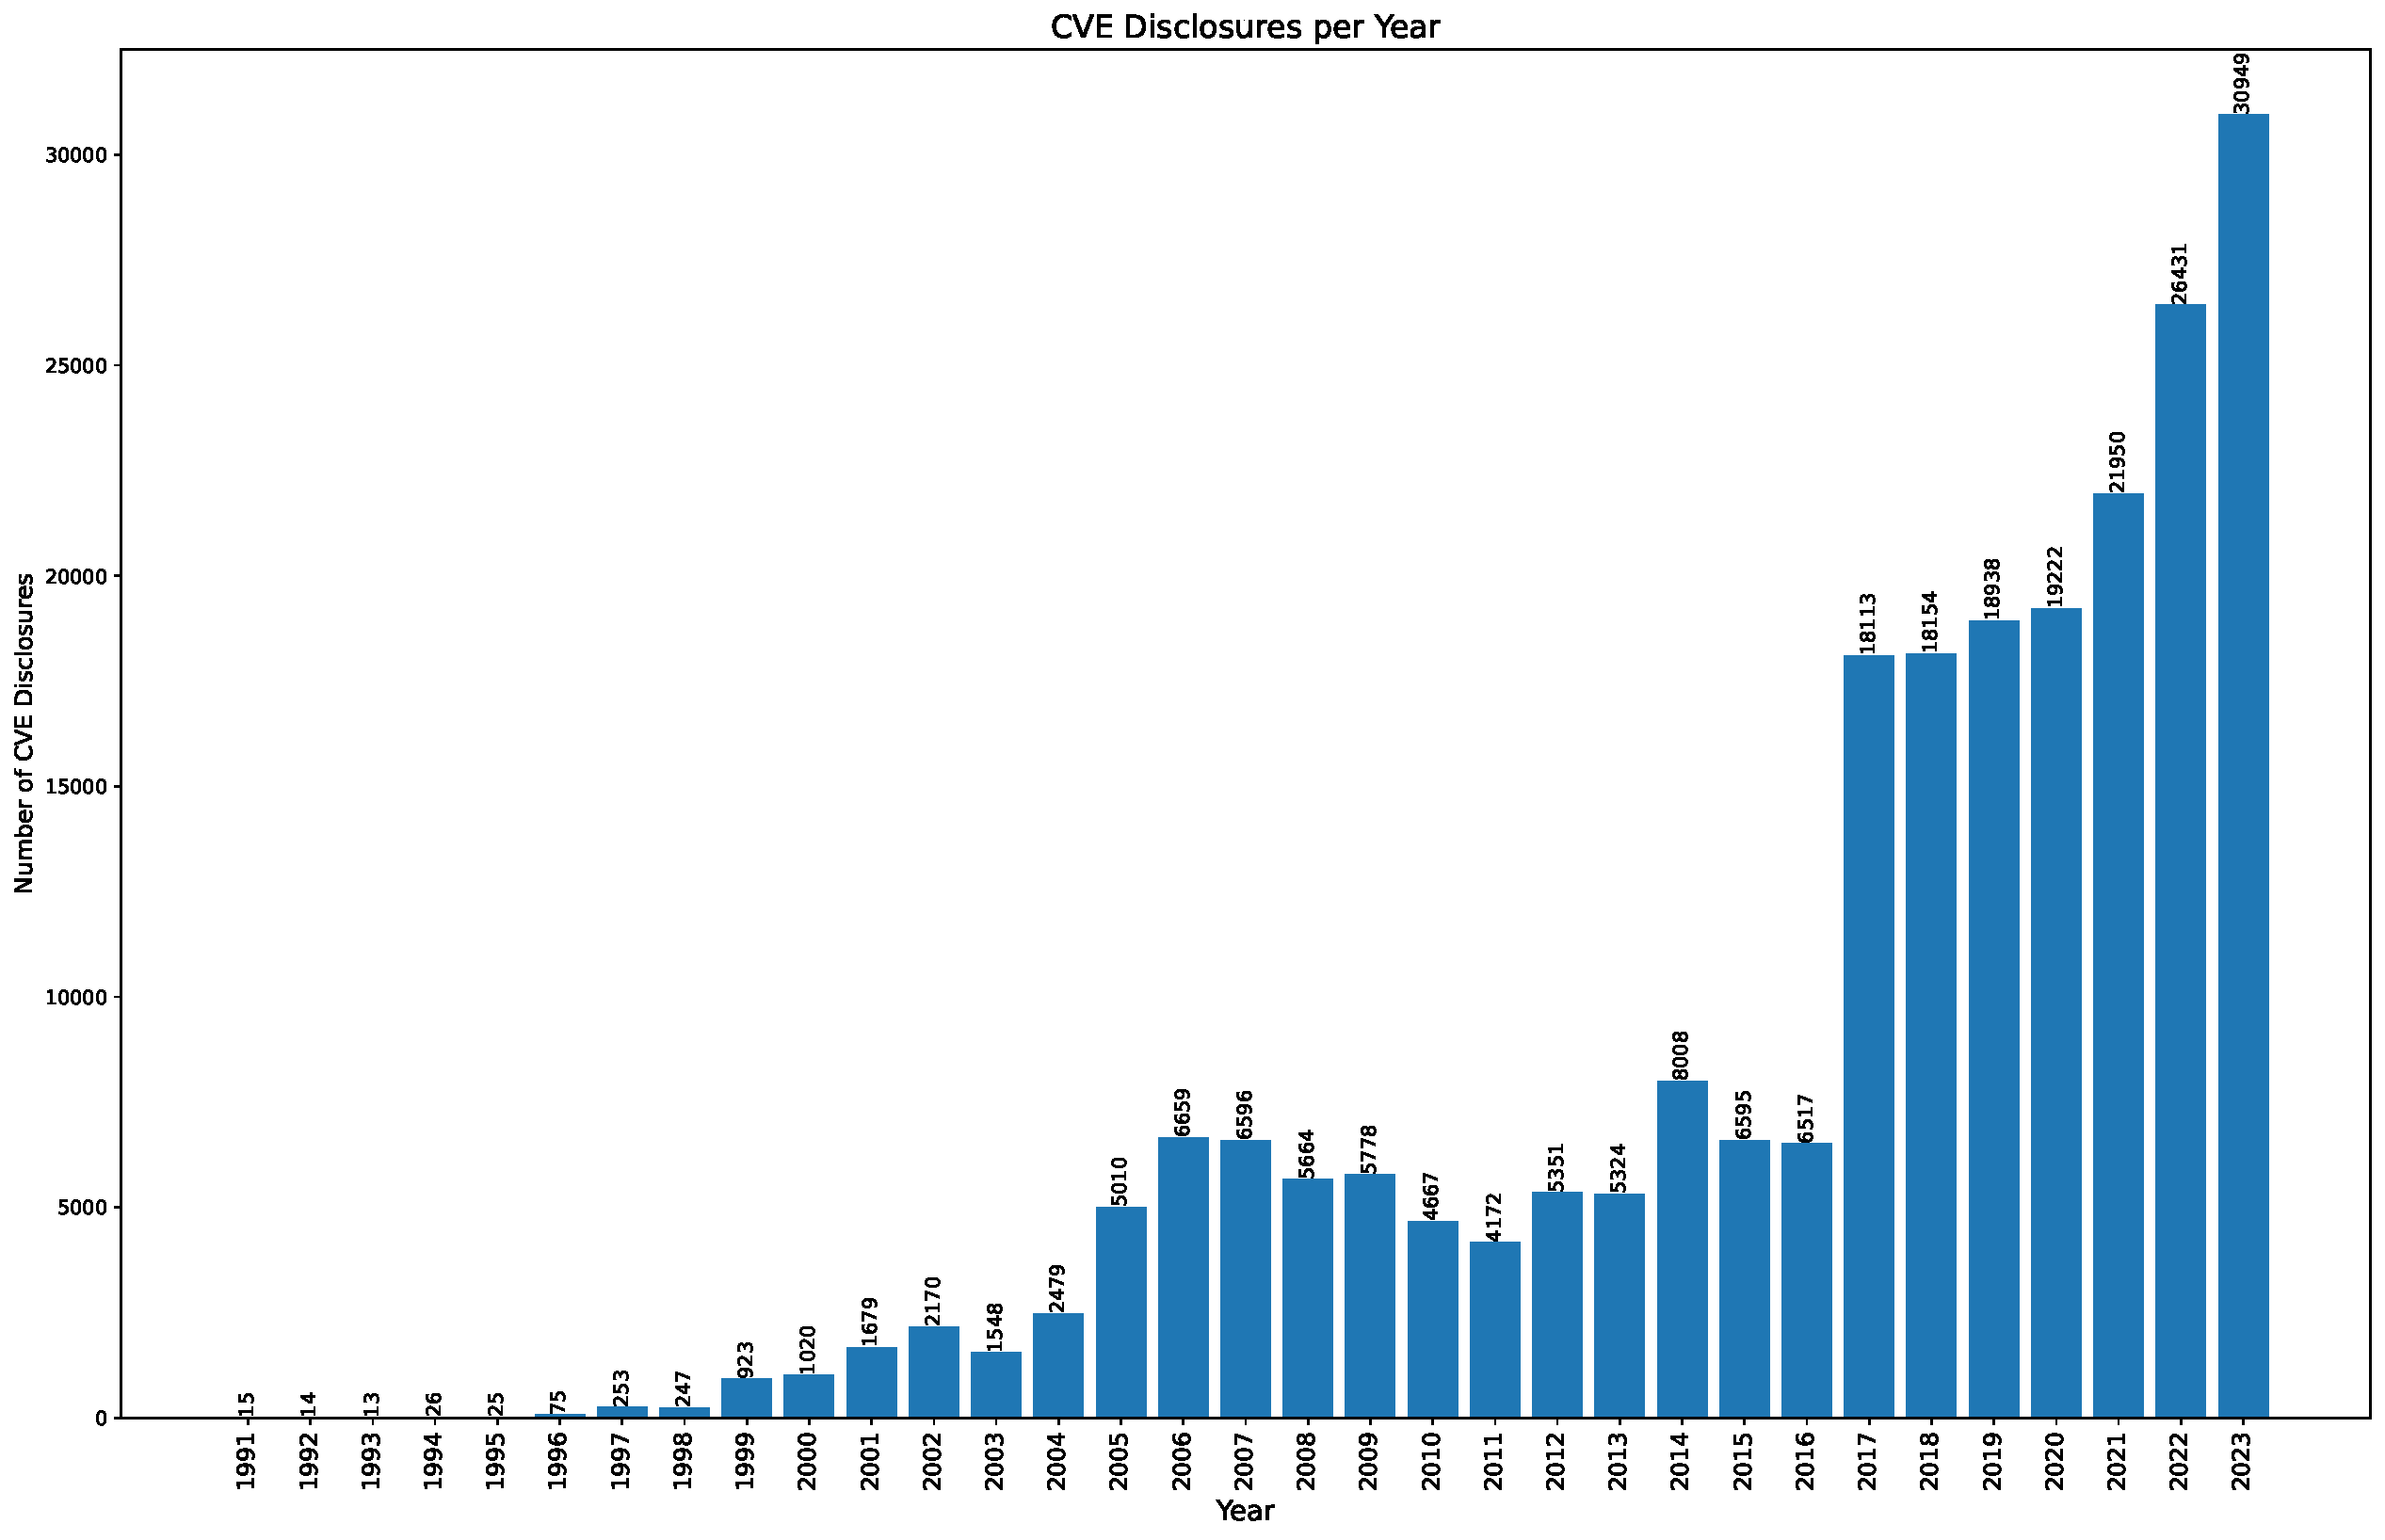
\includegraphics[width=0.8\textwidth]{figures/cves_per_year.pdf}
	\caption{\label{fig:cves_per_year}Number of new CVEs by year}
\end{figure}


\section{Background}

Vulnerabilities are stored in a consistent format called Common Vulnerabilities and
Exposures (CVE~\cite{CVE}).

\subsection{Here is an example CVE}
\begin{itemize}

	\item   Unique Identifier: CVE-2024-38526

	\item   Source: GitHub, Inc.

	\item   Published: 06/25/2024

	\item   Updated: 06/26/2024

	\item   Description: pdoc provides API Documentation for Python Projects. Documentation
	      generated with \texttt{pdoc --math} linked to JavaScript files from polyfill.io. The
	      polyfill.io CDN has been sold and now serves malicious code. This issue has been fixed in
	      pdoc 14.5.1\footnote{ Sourced from
		      \href{https://nvd.nist.gov/vuln/detail/CVE-2024-38526}{NVD CVE-2024-38526 Detail}
		      \cite{polyfill}}. \\

\end{itemize}

\bigskip

CVE reports have a unique identifier, which is given by one of the CVE numbering authorities (CNA~\cite{CNA}), such as
GitHub, Google or any of the \href{https://www.cve.org/PartnerInformation/ListofPartners}{CVE list of
	partners}~\cite{partners}.
The description is the most important part in our case. This should provide information about the
vulnerability. What can be exploited (device / software component)? How is the product affected if
the vulnerability is exploited? Ideally there would be a part of the description that relates to every metric,
unfortunately these descriptions are not necessarily suited to machine learning as the people
writing the descriptions are expecting a lot of intrinsic knowledge.

\subsection{The Common Vulnerability Scoring System}

CVSS scoring is a high level way to break up vulnerabilities into different categories.
Organisations can use it to choose which vulnerability to focus on first. CVSS is broken up into
three distinct sections: base, temporal and environmental scores.

For brevity I will only show the specifics of CVSS 3.1~\cite{CVSS_31} as this is by far the most commonly used
version, even if it is not the most recent.

\subsubsection{Base Score}

Below we summarise the
\href{https://www.first.org/cvss/v3.1/specification-document}{3.1 specification document
	provided by the  Forum of Incident Response and Security Teams (FIRST)}~\cite{CVSS_31}.


\begin{itemize}

	\item Attack Vector: Defines the avenues of attack that the vulnerability is open to. The more
	      open a component is, the higher the score. This can have the values: \texttt{Network},
	      \texttt{Adjacent}, \texttt{Local} and \texttt{Physical}.

	\item Attack Complexity: Describes how complex the attack is to orchestrate. Encompasses
	      questions like, what are the prerequisites? How much domain knowledge / background work is
	      necessary? How much effort does the attacker need to invest to succeed? This can have the
	      values: \texttt{Low} or \texttt{High}. \texttt{Low} gives a higher base score.

	\item Priviledges Required: The degree of privileges the user needs to complete the attack.
	      Ranging from: \texttt{None}, \texttt{Low} (e.g.\@ User level privilege), \texttt{High}
	      (e.g.\@ Administrator). The lower the privilege the higher the base score.

	\item User Interaction: Describes if the exploit requires another human user to make the attack
	      possible, e.g.\@ clicking a phishing link. This is either \texttt{None} or
	      \texttt{Required}, the score is highest when no user interaction is required.

	\item Scope: Defines if the attack can leak into other security scopes. For example, access to one
	      machine nay provide the ability to elevate privileges on other parts of the system. This can take
	      \texttt{Unchanged} or \texttt{Changed}, the score being highest when a scope change occurs.

	\item Confidentiality Impact: Detemines what is the impact on the information access /
	      disclosure to the attacker. This can be: \texttt{High}, \texttt{Low} or \texttt{None} with
	      \texttt{High} adding the most to the base score.

	\item Integrity Impact: Refers to the integrity of the information within the component, i.e.\@
	      could the data have been modified by the attacker. This has: \texttt{High}, \texttt{Low} or
	      \texttt{None}, as categories with \texttt{High} adding the most to the base score.

	\item Availability Impact: Refers to the impact of the attack on the availability of the
	      component, e.g.\@ the attacker taking the component off the network, denying the users
	      access. This can be: \texttt{High}, \texttt{Low} and \texttt{None} with \texttt{High} adding
	      the most to the base score.

\end{itemize}


\subsubsection{Temporal}

Below we again summarise from the
\href{https://www.first.org/cvss/v3.1/specification-document}{3.1 specification document
	provided by the Forum of Incident Response and Security Teams (FIRST)}~\cite{CVSS_31}.

\begin{itemize}

	\item Exploit Code Maturity: The state of the attack itself, e.g.\@ has this exploit been pulled
	      off in the wild or is it currently academic.

	\item Remediation Level: Whether the exploit in question has a patch available.

	\item Report Confidence: The degree of confidence in the CVE report itself, the report may be in
	      early stages where not all of the information is known.

\end{itemize}


\bigskip

Temporal metrics would be useful in general for a CVSS score, however NVD do not store these
temporal metrics. As far as I can tell there is no reason given for this specifically, though
discourse
\href{https://security.stackexchange.com/questions/270257/cvss-v3-and-v3-1-missing-temporal-metrics-exploit-code-maturity-and-remediation}{(Stack exchange post)}~\cite{stack_exchange} around the subject suggests that this is due to a lack
of verifiable reporting. From my perspective, both remidiation level and report confidence feel like
they could have scores attributed to them, however finding verifiable reports on the exploits seen
in the wild is difficult. There are two relatively new organisations trying to provide a solution to
this lack of verifiable reporting,
Cybersecurity \& Infrastructure Security Agency (CISA,
\href{https://www.cisa.gov/known-exploited-vulnerabilities-catalog}{public sector}) and
inthewild.org (\href{https://inthewild.io/}{private sector}~\cite{cisa}).

\subsection{Data Options}

I will be using NVD and MITRE as the sources of data. In 2016 when Johnson et al.\@ did their paper
on CVSS~\cite{bayes}, they had access to five different databases. Unfortunately only two of these
remain for modern data. There are others, but they are either in archival or proprietary status.

\subsubsection{National Vulnerability Database} \label{NVD_SECTION}

The National Vulnerability Database is the defacto standard dataset used for CVSS generation
research~\cite{costa, nvd_example1, nvd_example2}.  NVD being the standard makes a lot of sense as it is built
for the purpose with a team dedicated to enriching CVEs with CVSS scores. The dataset I am using was
retrieved using the NVD API in March 2024 and contains $\sim$100000 CVEs enriched with CVSS scores. This
comes in a consistently formatted JSON dump.

\subsubsection{MITRE Database}  \label{MITRE_SECTION}

MITRE is the defacto database for the storage of CVEs themselves, their database contains $\sim$40000
CVEs enriched with CVSS 3.1 scores. These are in a JSON dump retrieved in March 2024. The
format for usage is a bit more cumbersome. The CVSS scores are only stored as CVSS vector
strings (a simple text encoding~\cite{vector_string}). These are not hard to parse, though they are stored slightly
different between versions, as well as sometimes being inconsistent ($\sim$5000 had temporal metrics within
the vector strings in the MITRE database).



\begin{figure}
	\centering
	\makebox[\textwidth][c]{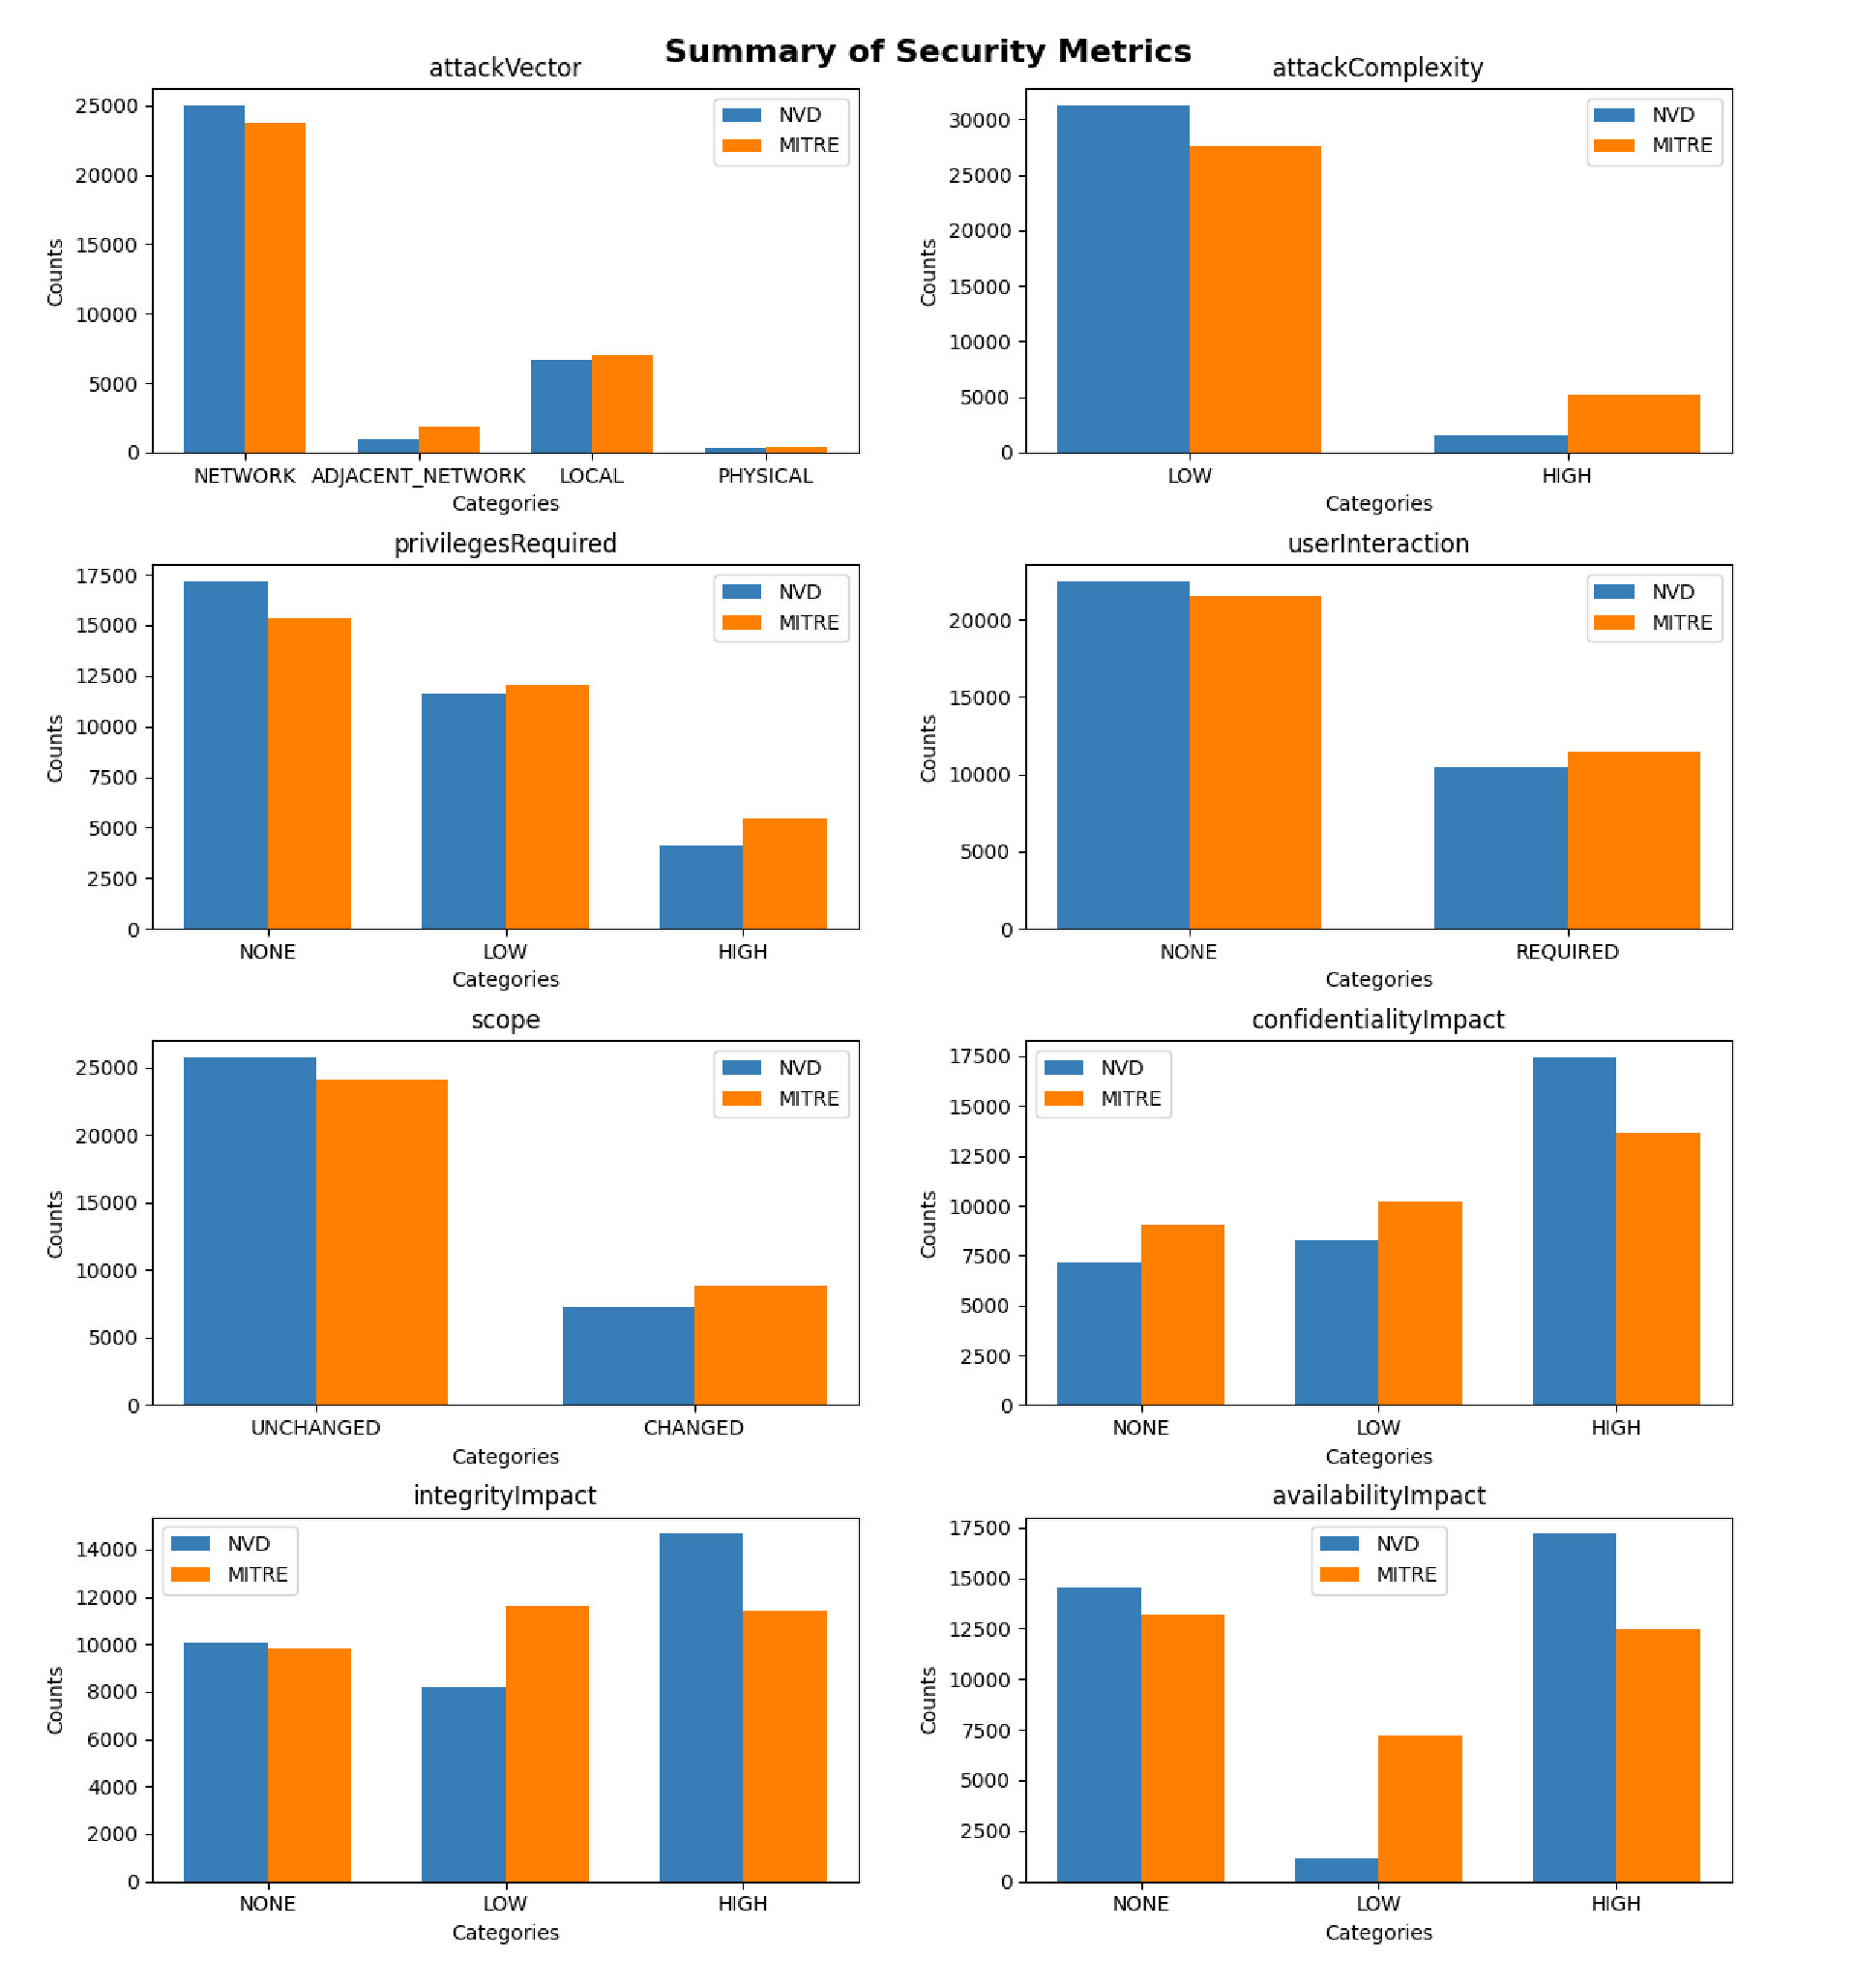
\includegraphics[width=1.2\textwidth]{figures/combined_overlap.pdf}}
	\caption{\label{fig:counts}Comparison of CVSS ratings between MITRE and NVD}
\end{figure}

\begin{figure}
	\centering
	\makebox[\textwidth][c]{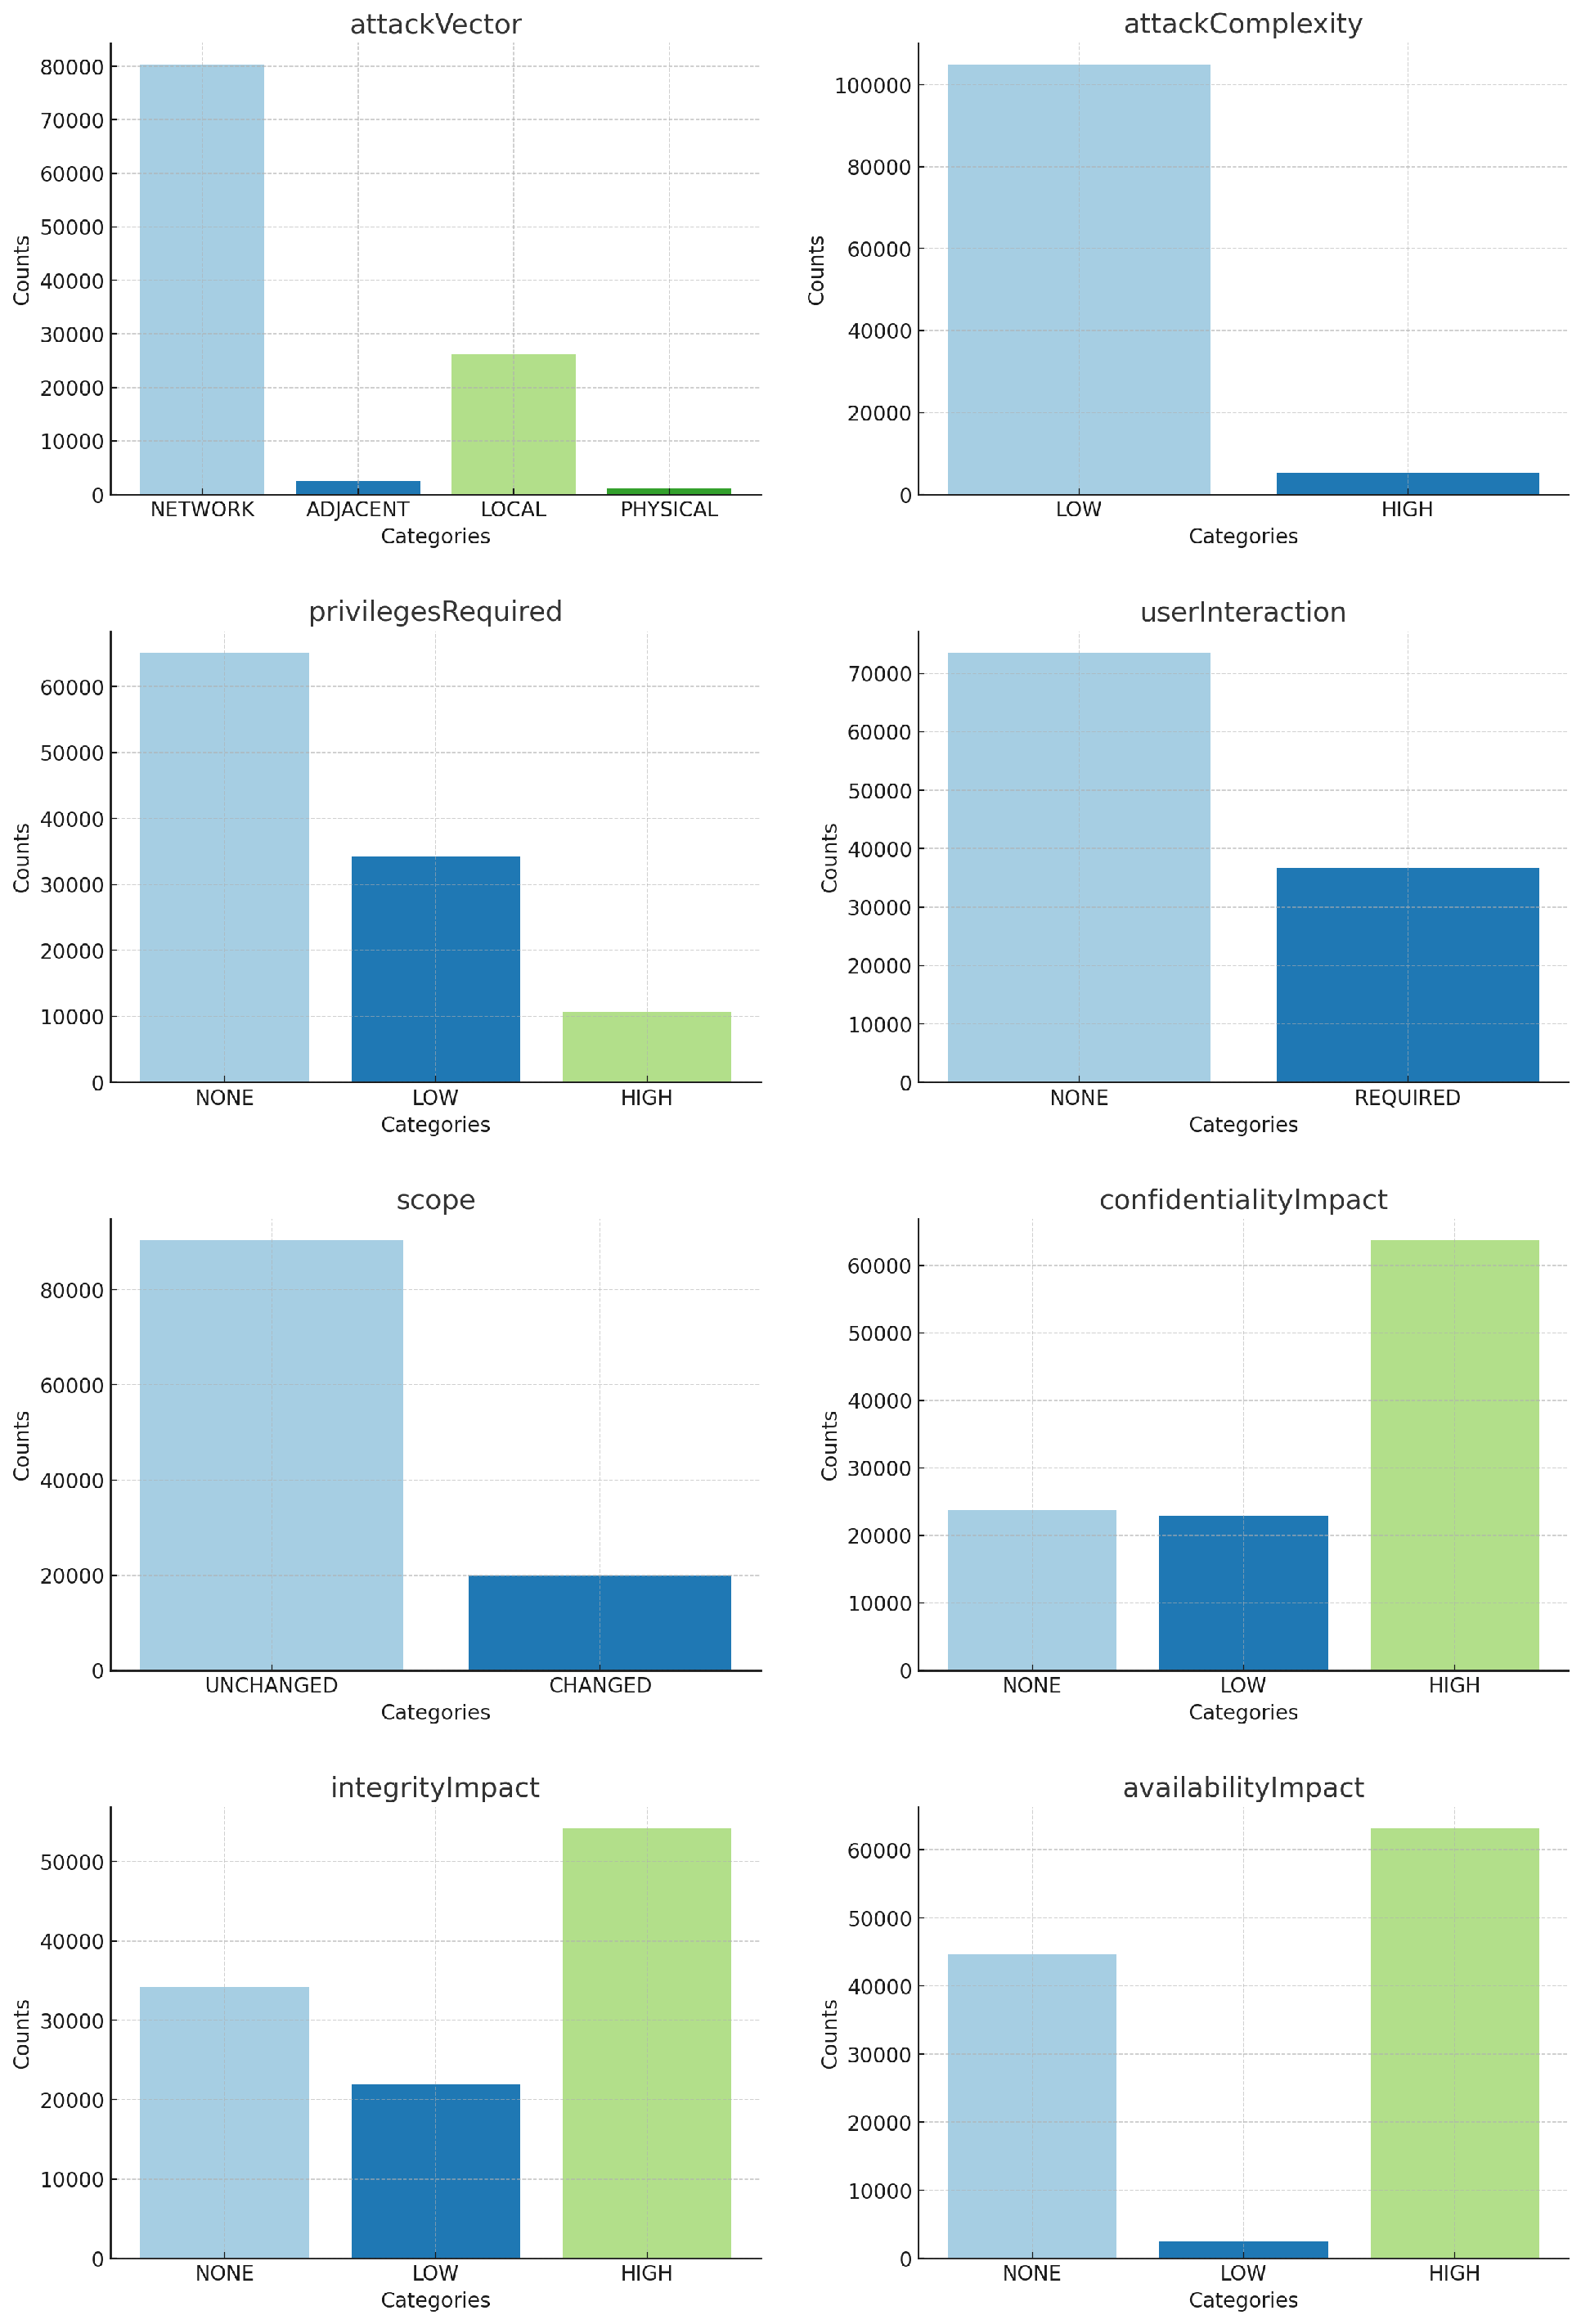
\includegraphics[width=0.8\textwidth]{figures/nvd_data.pdf}}
	\caption{\label{fig:nvd_data}Distribution of Metric ratings for NVD}
\end{figure}


\subsection{Evolution of CVSS and its Identity Crisis}
When CVSS 2.0 was released, it was promoted as a framework to help IT management prioritize and
remediate vulnerabilities posing the greatest risk. The initial goal was to provide a comprehensive
method for assessing risk, as indicated by its original documentation:
\\

\textit{\say{Currently, IT management must identify and assess vulnerabilities across many disparate
		hardware and software platforms. They need to prioritize these vulnerabilities and remediate those
		that pose the greatest risk. But when there are so many to fix, with each being scored using
		different scales, how can IT managers convert this mountain of vulnerability data into
		actionable information? The Common Vulnerability Scoring System (CVSS) is an open framework that
		addresses this issue.}}~\cite{CVSS_2}
\\

However, by the time CVSS 3.1 was released, the framework's focus had shifted, partly due to
complaints about CVSS being a poor judge of risk. The authors stated:

\textit{\say{CVSS measures severity, not risk.}}~\cite{CVSS_31}
\\

The identity crisis is a problem because the original stance, that it can be used as a primary
prioritisation tool, has lured parts of the industry into doing just that. As mentioned by Henry
Howland in~\cite{ubiquitous}, there are many large, mainly US based places mandating the sole use of
CVSS base score for remediation, such as the Payment Card Industry Data Security Standard~\cite{PCI}, the
Department of Defense Joint Special Access Program implementation Guide~\cite{DOD} to name a few.

This change in stance has created confusion about the true purpose of CVSS.

\subsubsection{CVSS Formula}


How CVSS is computed under-the-hood is confusing at best. CVSS 3.1 is not explained to the same
depth as version 2.0, but my understanding is that it followed a similar process. This is that
process summarised from
\href{https://www.first.org/cvss/v2/faq#Explanation-of-CVSS-v2-formula-and-metric-valued-development}{CVSS
	version 2 FAQ:}~\cite{CVSS_formula}


\begin{enumerate}
	\item  Divide the six metrics into two groups:

	      \begin{itemize}
		      \item \textbf{Impact} (3 metrics)
		      \item \textbf{Exploitability} (3 metrics)
	      \end{itemize}

	\item Create sub-vectors for each group:
	      \begin{itemize}
		      \item \textbf{Impact sub-vector}: 27 possible values ($3^3$)
		      \item \textbf{Exploitability sub-vector}: 26 possible values ($3^3 - 1$ for `no impact')
	      \end{itemize}

	\item Develop and apply a series of rules to order the sub-vectors. These rules
	      are primarily based on the severity of components, e.g.\@ vectors with more
	      \texttt{Complete}
	      components are rated higher.

	\item Assign scores to the ordered sub-vectors based on the derived rules and review by the
	      Special Interest Group (SIG).

	\item Apply weightings to the sub-vectors:
	      \begin{itemize}
		      \item \textbf{Impact}: 0.6
		      \item \textbf{Exploitability}: 0.4
	      \end{itemize}

	\item \label{formula_description} Develop a formula that approximates the scores derived from the ordered
	      sub-vectors. Ensure the formula produces scores with $\pm$0.5 error from the originally
	      defined vector score and does not exceed the maximum value of 10.

	\item Test and refine the formula through iterations, ensuring it aligns with desired values and
	      corrects any issues, such as scores exceeding 10.

\end{enumerate}

This process is inherently imprecise; it is not a system designed to give exact scores. As evidenced
by Item~\ref{formula_description} above, the formula (Equation~\ref{equation} shows the CVSS 3.1
base score formula for reference) that produces the score does not precisely match expert decisions.
The system incorporates considerable rounding and approximation, aiming to create a framework that
is both accessible and efficient for security professionals to use.

While CVSS serves a valuable purpose in vulnerability assessment, the limitations discussed
throughout this section highlight the potential pitfalls of relying solely on CVSS as a metric for
prioritization. However, as the major issues with CVSS relate to how the score is computed, there is
still value in the accuracy of the categorical scores themselves. This lead naturally on to
naturally lead us to question the consistency and reliability of CVSS scoring across different
organizations and databases. In the following section, we will explore this issue by examining the
scoring consistency between MITRE and NVD, two prominent sources of vulnerability information.

\section{Is there scoring consistency between MITRE and NVD?}

\subsection{Related Work}

The assessment and comparison of vulnerability scoring systems have been subjects of considerable
research in recent years. This section outlines key studies that have contributed to our
understanding of vulnerability scoring consistency, database reliability, and automated assessment
techniques.

\subsubsection{Comparative Analysis of Vulnerability Databases}

The primary work most closely aligned with our Bayesian analysis between MITRE and NVD is the study
by Johnson et al. entitled \say{Can the Common Vulnerability Scoring System be Trusted? A Bayesian
	Analysis}~\cite{bayes}. Conducted in 2016, this research investigated the state of CVSS databases
and their accuracy. Johnson et al.\@ found that NVD was the most reliable database and concluded
that the Common Vulnerability Scoring System could be trusted overall, as scorers rated CVEs
consistently. Their methodology forms the foundation for the database comparison in
Section~\ref{bayesian_modeling} of our study, although the specific results may have evolved since
their publication.

Dong et al.\@ \cite{dong} conducted a comprehensive study on detecting inconsistencies in public security
vulnerability reports. Their work, which analyzed vulnerability information from MITRE, NVD, and other
sources, highlighted the prevalence of information inconsistencies and developed an automated system
to detect such inconsistencies. This research underscores the importance of maintaining accurate and
consistent vulnerability information across different databases and reports.

\subsubsection{Automated Vulnerability Assessment Techniques}

Jiang and Atif's work, \say{An Approach to Discover and Assess Vulnerability Severity Automatically in
	Cyber-Physical Systems}~\cite{jiang}, presents an innovative pipeline for vulnerability assessment.
Their approach utilizes multiple data sources and employs a majority voting system to mitigate the
impact of incorrectly scored CVEs. While their methods differ from our focus on database comparison,
their work underscores the value of leveraging multiple data sources in vulnerability assessment.


\subsubsection{Consistency and Reliability of CVSS Scoring}

Allodi and Massacci~\cite{allodi} conducted a critical examination of CVSS scoring in their paper
\say{Comparing Vulnerability Severity and Exploits Using Case-Control Studies.} Their research questions
the correlation between CVSS scores and the actual exploitation of vulnerabilities in the wild,
raising important considerations about the practical implications of vulnerability scoring systems.

Furthermore, Spring et al.~\cite{improving_cvss} investigated the reliability of CVSS scoring across
different human raters in their study \say{Towards Improving CVSS.} They found significant variations in
how different individuals interpret and apply CVSS scoring guidelines, highlighting the challenges
in achieving consistent vulnerability assessments even within a standardized framework.

\subsubsection{Summary}

These studies collectively demonstrate the ongoing challenges and advancements in vulnerability
scoring and database reliability. While Johnson et al.~\cite{bayes} provided a foundational analysis
of CVSS trustworthiness, subsequent research has explored automated techniques, cross-database
comparisons, and the practical implications of vulnerability scores. This study builds upon
this body of work, focusing specifically on the consistency between MITRE and NVD scoring using
updated data and methodologies.

\subsection{Priliminary Data exploration}

To enable a direct comparison between NVD and MITRE scoring practices, we performed necessary data
preprocessing steps. CVE entries from both sources were aligned and normalized to ensure consistency
in format and metric representation. Figure~\ref{fig:counts} presents the resulting comparison of
NVD and MITRE scores across various CVSS metrics.

Analysis of the processed data reveals:

\begin{itemize}

	\item NVD and MITRE scorers generally rate CVEs similarly, indicating broad consensus in
	      vulnerability assessment.

	\item NVD tends to assign the most common categorical value more frequently for each metric,
	      while MITRE's ratings show a wider distribution (Figure~\ref{fig:counts}).

	\item Significant discrepancies exist for certain metrics, notably \texttt{Attack Complexity},
	      where MITRE assigns \texttt{Low} scores more frequently than NVD.

\end{itemize}

These observations highlight the challenges inherent in vulnerability rating systems. While a \say{true}
value for each metric theoretically exists, comprehensive assessment requires extensive domain
knowledge, which can vary between scorers. Our machine learning model, though lacking direct access
to this knowledge, aims to learn these nuances by analyzing patterns across numerous
vulnerabilities.

% The scorers for both NVD and MITRE do rate CVEs reasonably similarly. One pattern you can see as
% shown by Figure~\ref{fig:counts}, is that NVD generally give\notedme{grammar} the most common
% categorical output more ratings. They are less spread out across the full range of values. In
% addition, if we look at the \texttt{Attack Complexity} metric, there is a reasonably large
% difference in how they are rated, MITRE rate a lot more of the metrics with a \texttt{Low} score.
% This points to some of the difficulty with this kind of rating system, while in theory there is a
% true value for these metrics, it requires knowledge of the whole space around each of the
% vulnerabilities, this knowledge will always vary marker to marker. The model will not have direct
% access to this knowledge; however, it is hoped that it will be able to trace relationships between
% the different vulnerabilities and learn this intrinsically.

\subsection{Hierarchical Bayesian Model} \label{bayesian_modeling}

Analysis between the NVD~\cite{NVD} and MITRE~\cite{MITRE} databases is conducted using a
hierarchical Bayesian model. This model type is particularly suitable when the population is
expected to share similarities in some respects while differing in others. In this context, while
the databases share common knowledge about vulnerabilities, they differ in the experience of the
individuals rating the metrics~\cite{bayes}.

The model builds upon the original framework presented in Section 4.1 of~\cite{bayes}. It assumes
the existence of a true value for each CVSS dimension, acknowledging that the database sample may
deviate from this true value. These potential inaccuracies are represented using confusion matrices
(see Equation~\ref{confusion_matrix_formula}).

A key distinction from the original model is the variability in the number of categorical choices
for each CVSS metric. While the original model consistently used three variables for each CVSS
metric, my adapted model accommodates between two to four categorical choices, depending on the
specific CVSS dimension being evaluated.

\subsubsection{Confusion Matrix}

Below is an example of the confusion matrix for the CVSS dimension \texttt{Confidentiality Impact}:

\begin{equation}\label{confusion_matrix_formula}
	\Pi_{ci} = \begin{bmatrix}
		\pi_{nn} & \pi_{nl} & \pi_{nh} \\
		\pi_{ln} & \pi_{ll} & \pi_{lh} \\
		\pi_{hn} & \pi_{hl} & \pi_{hh} \\
	\end{bmatrix}
\end{equation}

where $\pi_{nn}$ denotes the probability that the database correctly assigns the score \texttt{None}
when the actual value is indeed \texttt{None}. Conversely, $\pi_{nl}$ and $\pi_{nh}$ represent
instances where \texttt{None} was not the true value, indicating an incorrect score assignment by
the database.

\subsubsection{Prior Distributions}

For categorical variables, we employ uninformative priors using Dirichlet distributions~\cite{dirichlet}. This
approach provides a uniform prior over the probability space for all categorical options, minimizing
the influence of prior beliefs on the results. The impact of these priors is negligible for
categorical metrics with more options than the number of categories.

The confusion matrices also utilize Dirichlet distribution priors. However, we incorporate a slight
initial belief to reflect that the individuals producing scores are not acting entirely randomly and
are likely to be correct more often than not. These priors remain weak given the thousands of
observations in our dataset.

\subsubsection{Parameter Estimation}

Our parameter estimation follows the Bayesian approach, updating prior beliefs with observations to
produce posterior beliefs. We employ Markov Chain Monte Carlo (MCMC~\cite{mcmc}) methods, which allow for
simulating data based on the previously created distribution by sampling values that the model
believes are likely from the target distribution. This technique enables accurate sampling without
requiring all data points.

For implementation, we utilized the PyMC library~\cite{pymc}, which fulfills the same functions as
JAGS in the original paper~\cite{bayes}. PyMC facilitates the modeling process and provides robust
tools for Bayesian inference and MCMC sampling.

This methodology provides a comprehensive framework for analyzing and comparing vulnerability
scoring across different databases, accounting for the inherent uncertainties and variations in
expert assessments.


\subsubsection{Bayesian Analysis Results}

The database analysis results, presented through confusion matrices, corroborate the observations
made in Figure~\ref{fig:counts} regarding NVD and MITRE scoring patterns. Key findings include:

\begin{itemize}
	\item NVD consistently demonstrates higher accuracy for the most common categories in each metric,
	      aligning with its tendency to favor dominant categorizations as observed in Figure~\ref{fig:counts}.

	\item The disparity in scoring is particularly evident in metrics like \texttt{Attack Complexity}, where
	      NVD shows higher accuracy for the more frequent \texttt{Low} option (98\%) compared to
	      MITRE (87\%).

	\item MITRE's scoring exhibits a more balanced distribution across categories, consistent with the wider
	      spread of ratings seen in Figure~\ref{fig:counts}.
\end{itemize}

These quantitative results confirm the visual patterns observed in Figure~\ref{fig:counts},
providing a numerical basis for the scoring differences between NVD and MITRE. While the overall
estimated accuracy for both databases is lower than in previous studies~\cite{bayes}, the relative
performance and tendencies remain consistent with our initial observations.

\bigskip

\begin{figure}[H]
	\centering
	\makebox[\textwidth][c]{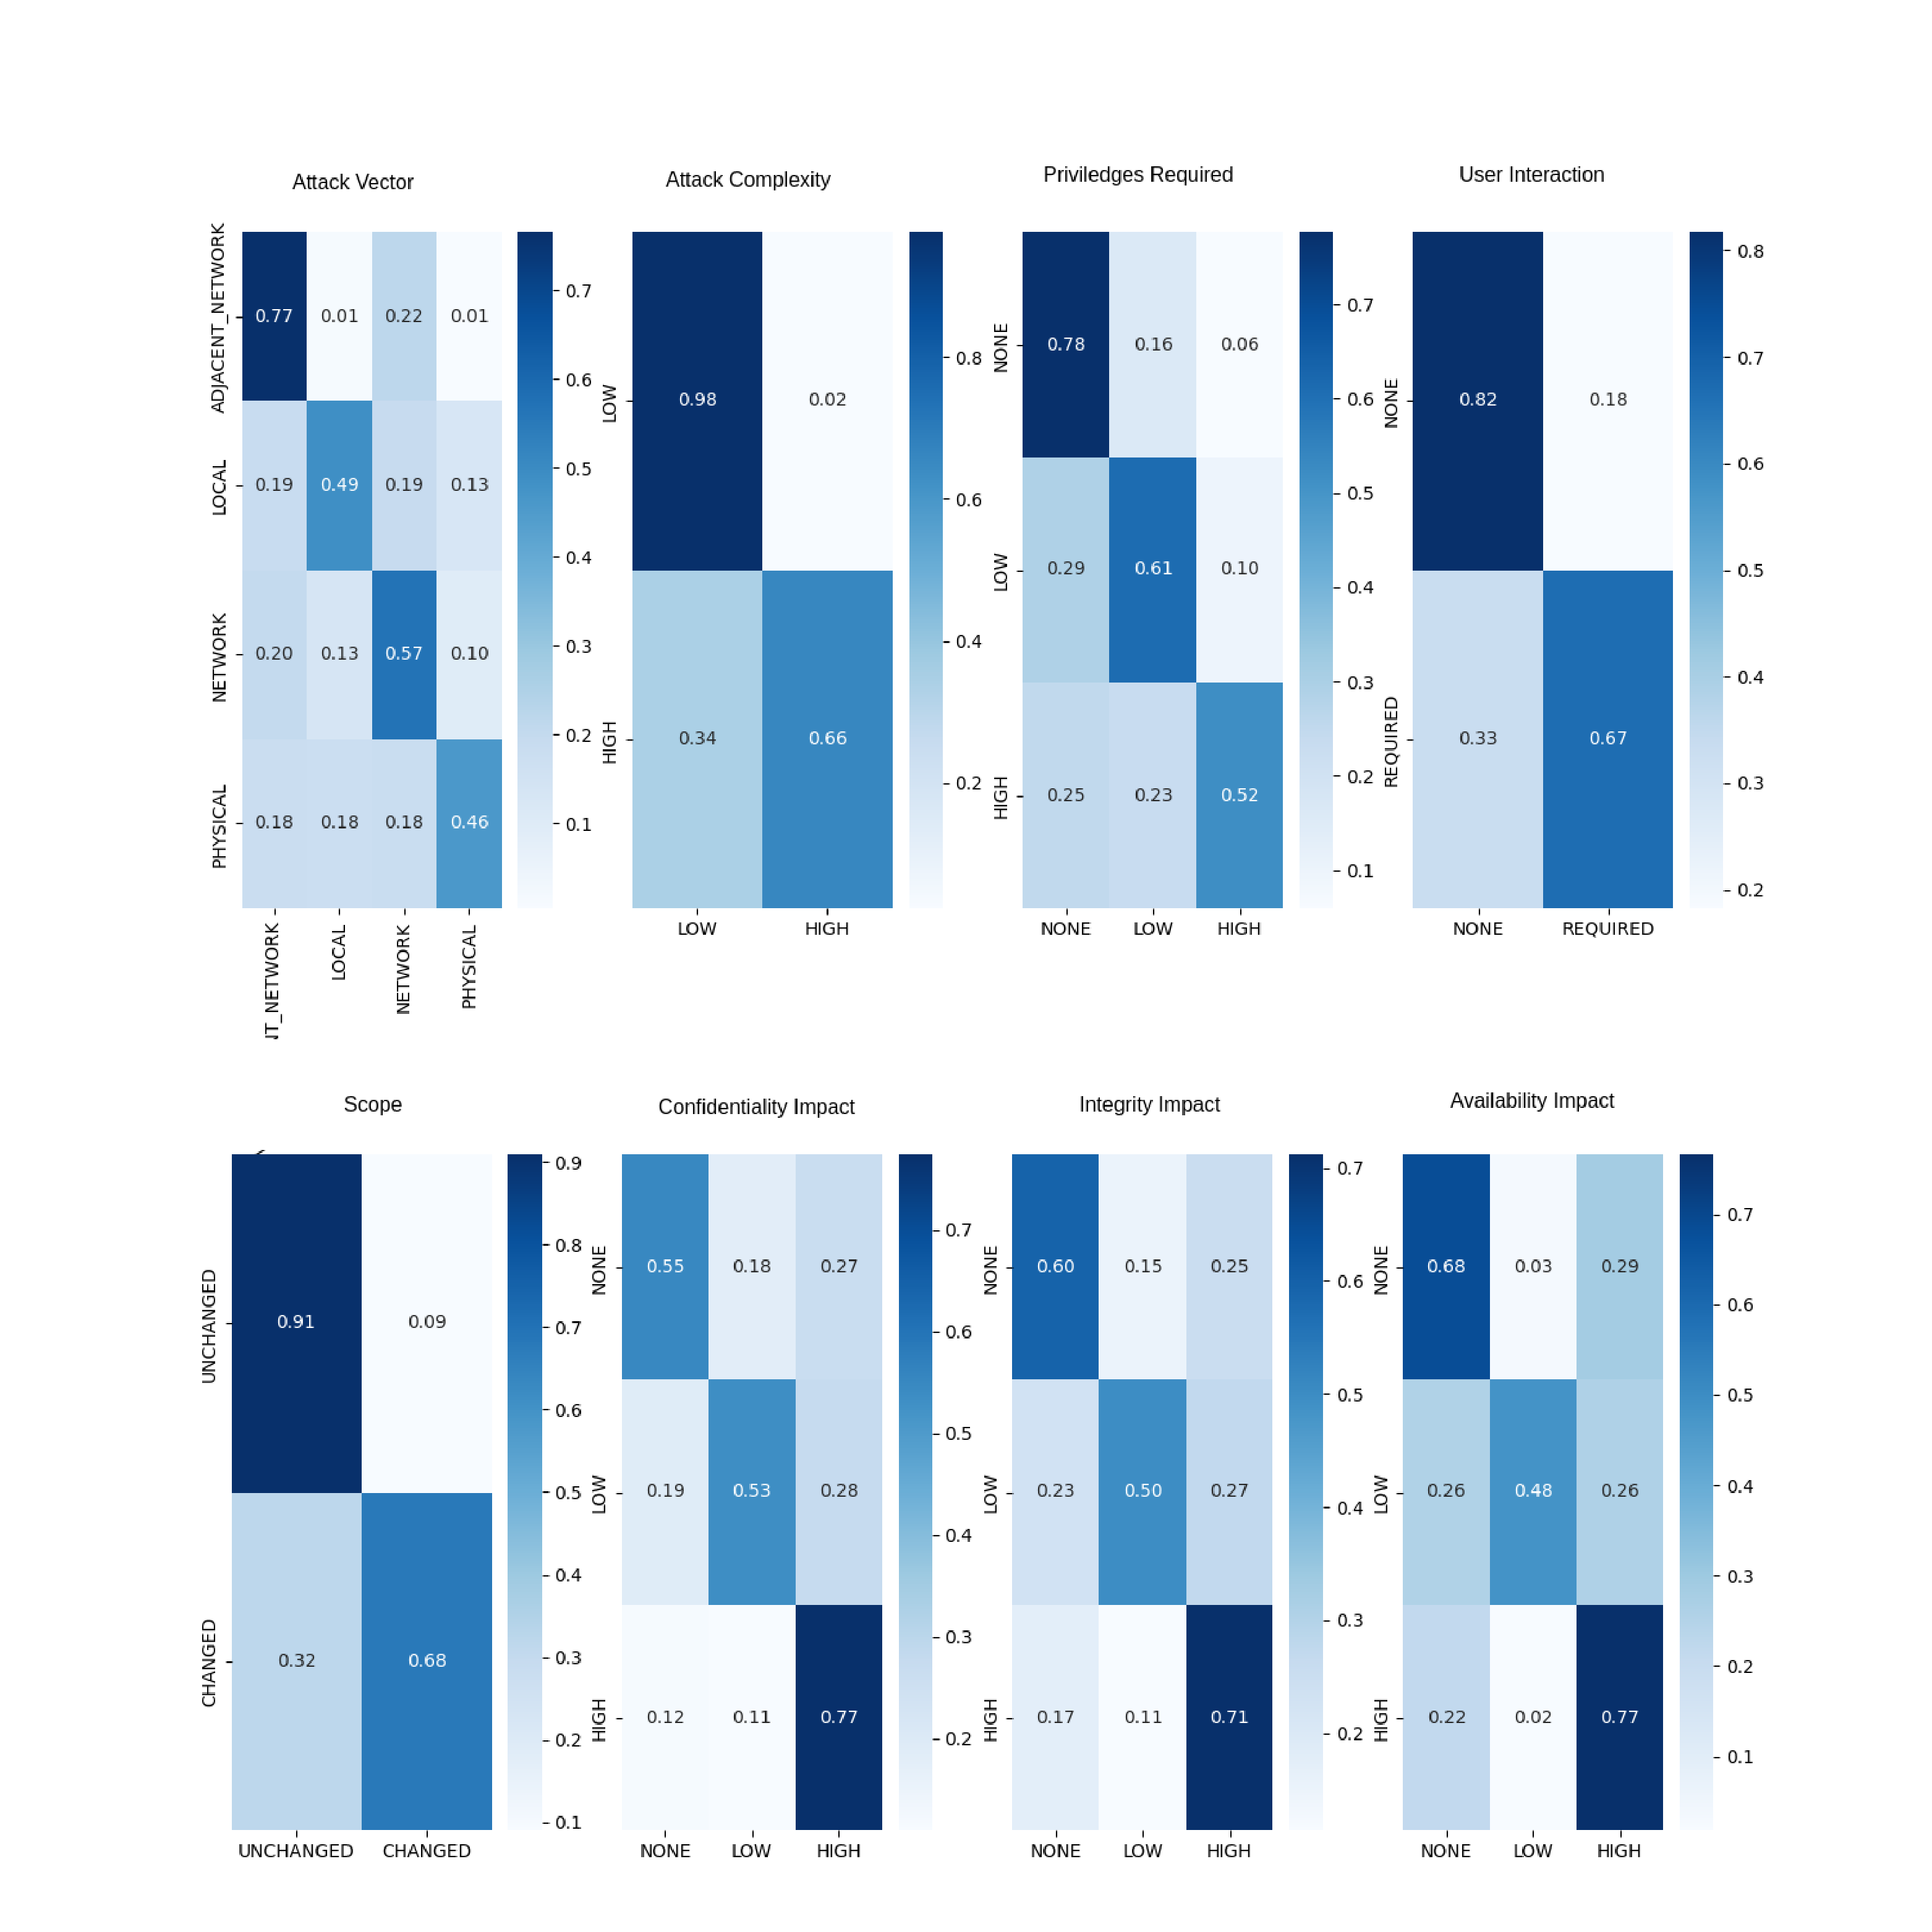
\includegraphics[width=1.2\textwidth]{figures/nvd_31_titles.pdf}}
	\caption{\label{fig:nvd_31_confusion_matrices}Confusion Matrices for NVD for CVSS version 3.1}
\end{figure}

\begin{figure}[H]
	\centering
	\makebox[\textwidth][c]{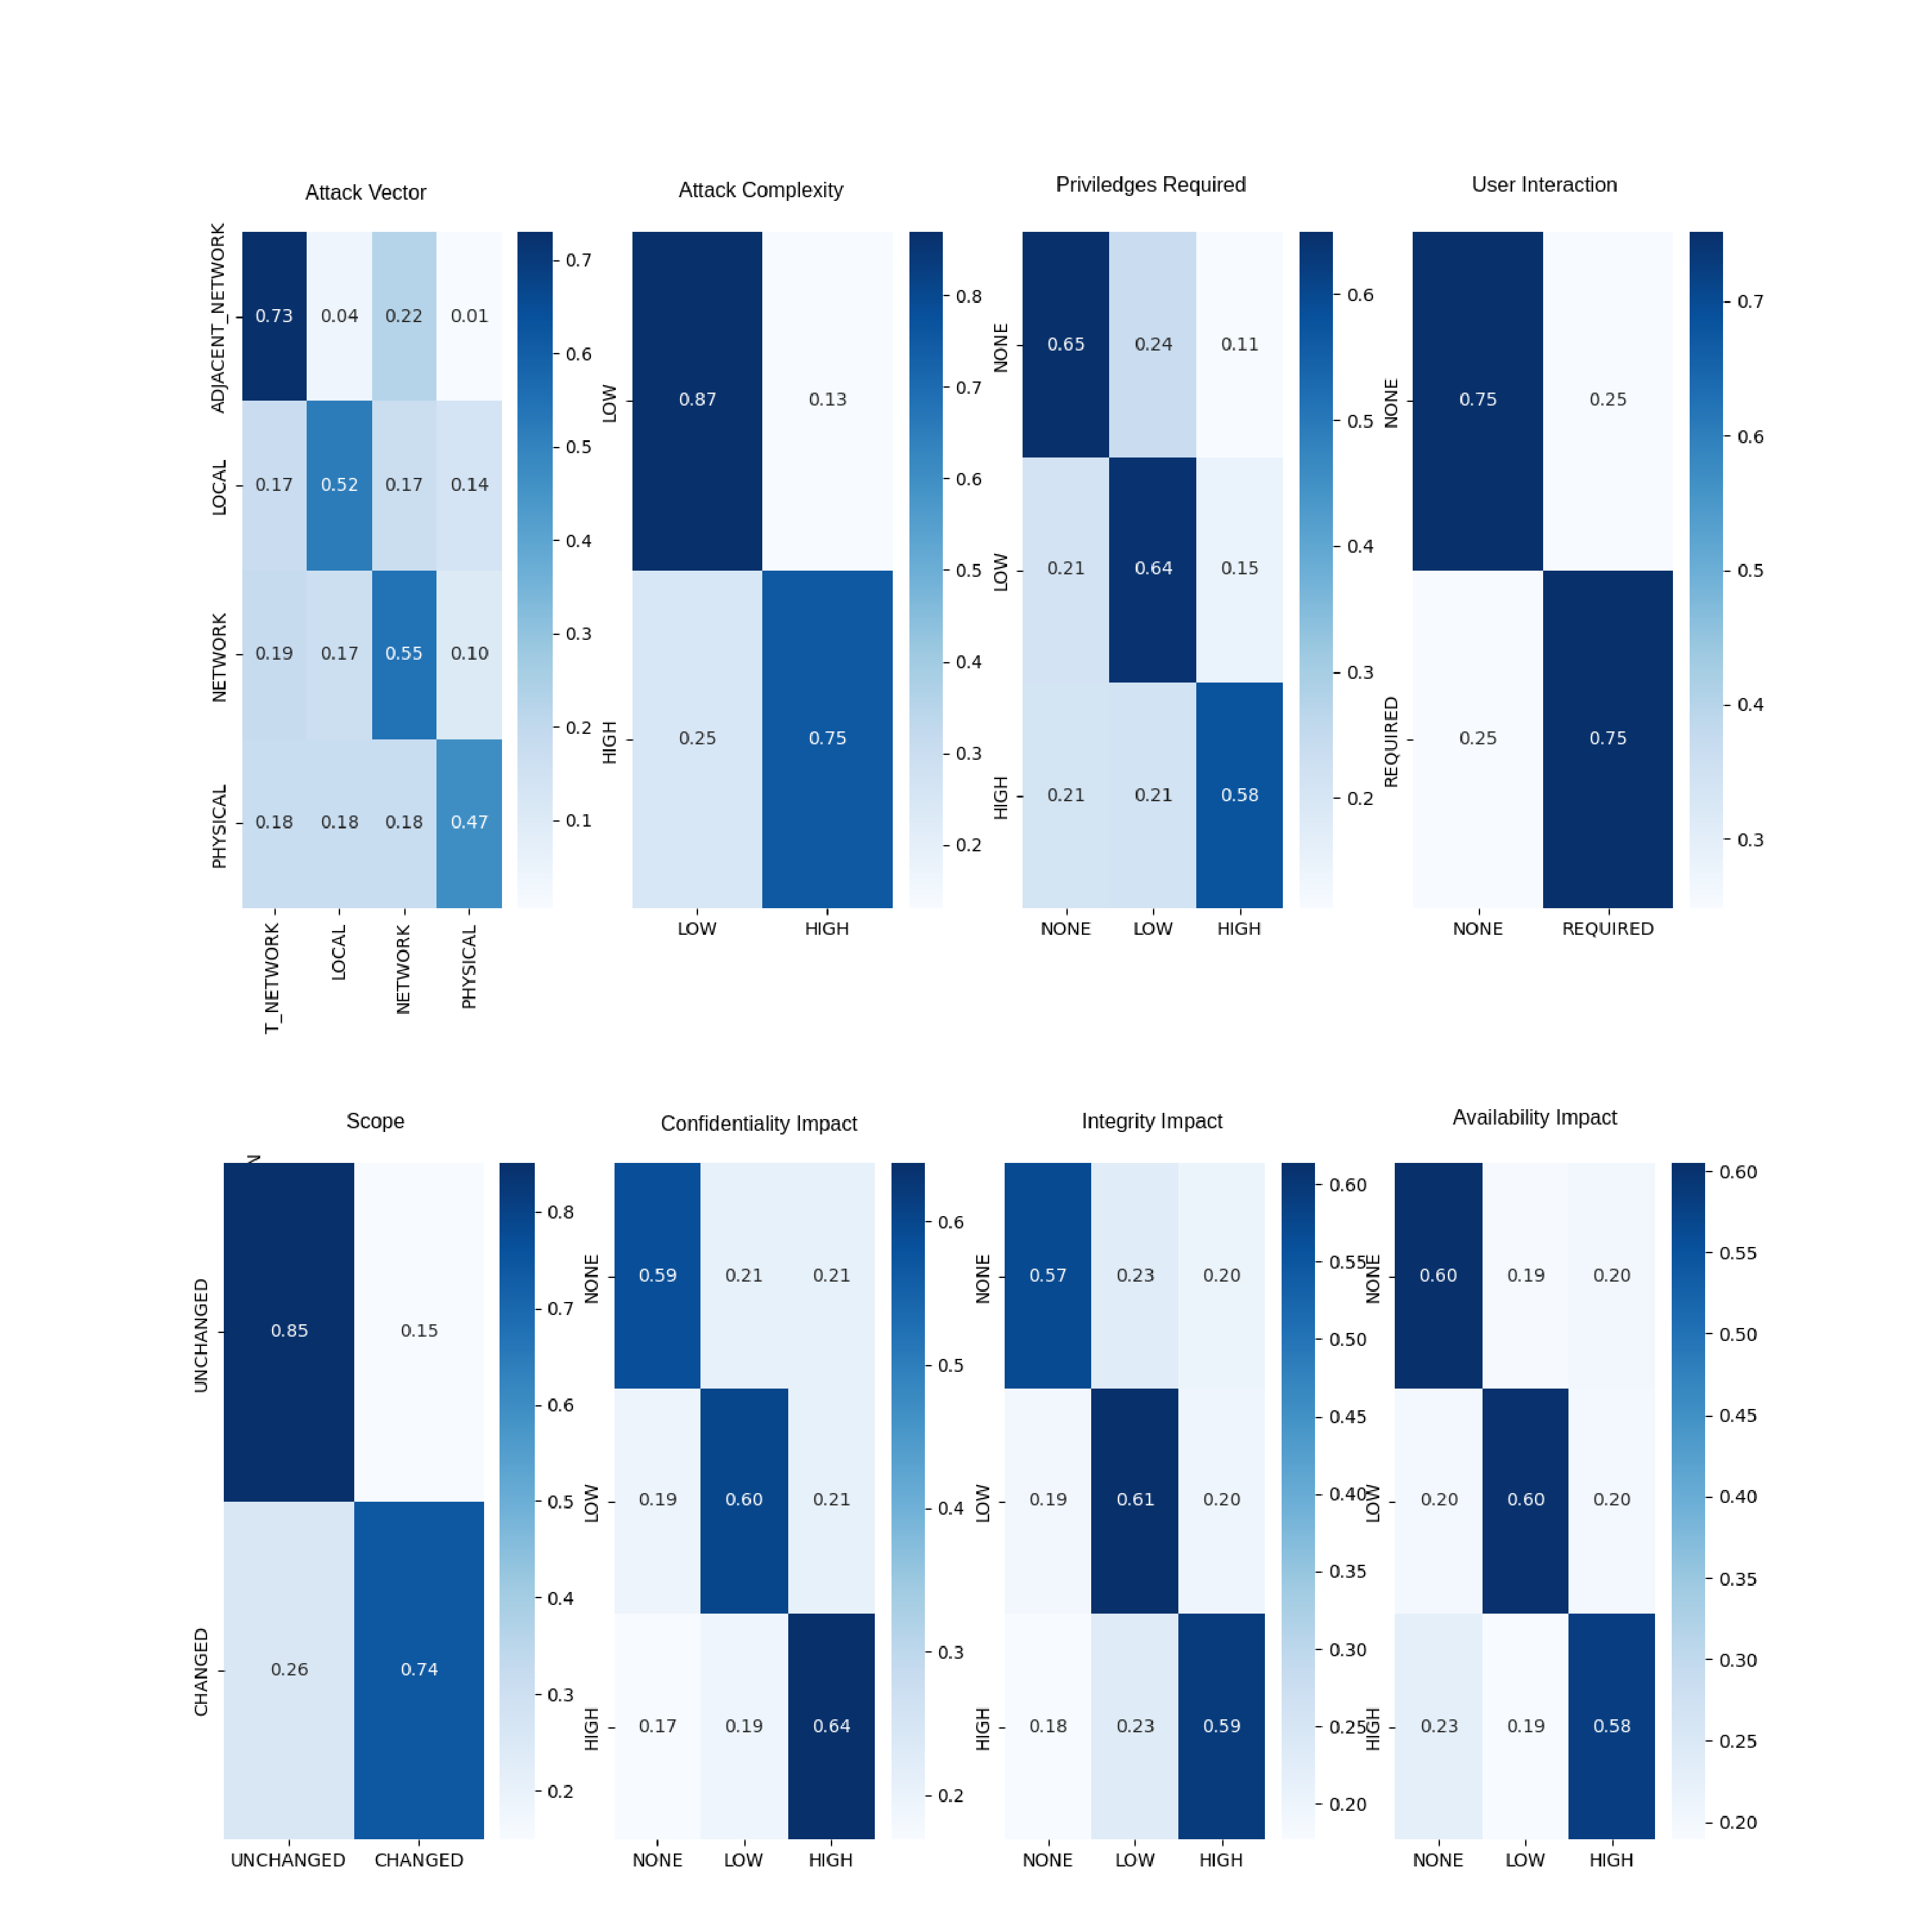
\includegraphics[width=1.2\textwidth]{figures/mitre_31_titles.pdf}}
	\caption{\label{fig:mitre_31_confusion_matrices}Confusion Matrices for MITRE for CVSS version 3.1}
\end{figure}

% \begin{table}
% 	\centering
% 	\caption{\label{tab:johnson_confusion_matrices}Confusion Matrices for NVD on CVSS version 2.0 from Johnson et al.\@ \cite{bayes}}
% 	\[
% 		\begin{array}{c|c}
% 			\textbf{Access vector}  & \textbf{Access complexity} \\
% 			\hline
% 			\begin{tabular}{l|ccc}
% 				  & N    & A    & L    \\
% 				\hline
% 				N & 0.99 & 0    & 0    \\
% 				A & 0.21 & 0.71 & 0.08 \\
% 				L & 0.05 & 0.0  & 0.95 \\
% 			\end{tabular}
% 			                        &
% 			\begin{tabular}{l|ccc}
% 				  & L    & M    & H    \\
% 				\hline
% 				L & 0.54 & 0.29 & 0.17 \\
% 				M & 0.02 & 0.88 & 0.1  \\
% 				H & 0.01 & 0.08 & 0.91 \\
% 			\end{tabular}
% 			\\
% 			\textbf{Authentication} & \textbf{Confidentiality}   \\
% 			\hline
% 			\begin{tabular}{l|ccc}
% 				  & N    & S    & M    \\
% 				\hline
% 				N & 0.99 & 0.01 & 0    \\
% 				S & 0.04 & 0.95 & 0.01 \\
% 				M & 0.19 & 0.2  & 0.6  \\
% 			\end{tabular}
% 			                        &
% 			\begin{tabular}{l|ccc}
% 				  & C   & P    & N    \\
% 				\hline
% 				C & 0.4 & 0.2  & 0.2  \\
% 				P & 0.2 & 0.4  & 0.19 \\
% 				N & 0.2 & 0.21 & 0.4  \\
% 			\end{tabular}
% 			\\
% 			\textbf{Integrity}      & \textbf{Availability}      \\
% 			\hline
% 			\begin{tabular}{l|ccc}
% 				  & C    & P    & N    \\
% 				\hline
% 				C & 0.91 & 0.08 & 0.01 \\
% 				P & 0.05 & 0.93 & 0.02 \\
% 				N & 0.02 & 0.07 & 0.92 \\
% 			\end{tabular}
% 			                        &
% 			\begin{tabular}{l|ccc}
% 				  & C    & P    & N    \\
% 				\hline
% 				C & 0.92 & 0.07 & 0.01 \\
% 				P & 0.07 & 0.91 & 0.02 \\
% 				N & 0.02 & 0.11 & 0.87 \\
% 			\end{tabular}
% 		\end{array}
% 	\]
% \end{table}


\section{Can we improve the LLMs' classifier performance when we augment the NVD dataset with data
  from the MITRE dataset?}\label{cvss_prediction}

\notedme{Normally every section should have some lead-in text here. Also, the section title is really long.}

\subsection{Related Work}

Recent advancements in natural language processing and machine learning have led to significant
progress in automating CVSS metric prediction from vulnerability descriptions. This area of research
is particularly relevant to our work in Section \ref{cvss_prediction}\notedme{... sounds like a reference pointing elsewhere, but this \emph{is} section 4. This is probably what I'd expect the lead-in text to discuss.}.

Shahid and Debar \cite{cvss_bert} proposed CVSS-BERT, an approach leveraging state-of-the-art
natural language processing techniques to determine the severity of a computer security
vulnerability from its description. Their work, titled \say{CVSS-BERT: Explainable Natural Language
	Processing to Determine the Severity of a Computer Security Vulnerability from its Description,}
uses multiple BERT classifiers, one for each metric composing the CVSS vector. This approach is
similar to our methodology in Section \ref{cvss_prediction}\notedme{Again needs not to sound like this text has been moved here from a different section.}.

The authors of CVSS-BERT trained their model on CVE vulnerability data from 2018 to 2020, using
BERT-small, a lighter version of BERT. They achieved high accuracy for predicting individual CVSS
metrics, ranging from 83.79\% to 96.07\%. For 55.3\% of the vulnerabilities in their test set, the
predicted severity scores exactly matched the true severity scores. Their work also emphasized
explainability, using gradient-based input saliency methods to determine the most relevant input
words for each prediction.

Our work builds upon the foundations laid by CVSS-BERT, exploring the impact of augmenting the
training data with additional sources (MITRE dataset) to potentially improve the model's
performance. We aim to investigate whether this augmentation can lead to more accurate and robust
CVSS predictions.

Costa et al.~\cite{costa} also contributed to this field with their paper \say{Predicting CVSS Metric
	via Description Interpretation.} They tested various large language encoder-only models for
generating CVSS from CVE descriptions, achieving state-of-the-art results with the DistilBERT model.
Their work included text preprocessing techniques and explored the interpretability of the models
using Shapley values, providing additional perspectives on enhancing CVSS prediction accuracy and
explainability.

These studies collectively demonstrate the potential of transformer-based models in vulnerability
assessment and highlight the challenges in accurately predicting CVSS metrics from textual
descriptions. Our work in Section~\ref{cvss_prediction}\notedme{again with the \S\ref{cvss_prediction} issue} builds upon these foundations, particularly
the approach of CVSS-BERT, while exploring the impact of augmenting the training data with
additional sources to potentially improve prediction accuracy and robustness.

Cody Airey---a classmate of mine---has been working on a similar problem. He has been repoducing
results from Costa et al.\@~\cite{costa}, I am choosing to use Airey's results due to them being on
CVSS version 3.1 instead of a mix of versions 3.0 and 3.1 as Costa et al.\@ used. My choice of model
for CVSS prediction will very much bootstrap off his work. So far, a strong contender for
state-of-the-art model for predicting CVSS metrics from CVE descriptions is the DistilBERT
model~\cite{distilbert}. This is a variant of BERT~\cite{BERT}, a pre-trained deep bidirectional
transformer large language model developed by Google. DistilBERT has advantages over other BERT
models in terms of performance, but also on speed of training as well as size / memory footprint of
the model.

\subsubsection{Training}

The model is trained separately for each of the eight CVSS metrics. To ensure robustness and
reliability of our results, we trained each model on five different data splits. This approach
allows us to calculate standard deviations, effectively mitigating the impact of any potential
\say{lucky} data split on our findings.

Our work diverges from Costa et al.\@ and Airey's approaches by utilizing a combined dataset from both
NVD and MITRE, rather than relying solely on NVD data. We converted this merged data into a CSV
format, containing vulnerability descriptions and their corresponding CVSS scores. This integration
resulted in approximately 40,000 duplicate CVEs and a total of around 140,000 CVEs enriched with
CVSS scores. Table~\ref{tab:distil_part1} and Table~\ref{tab:distil_part2} present the performance
results of our DistilBERT model trained on this combined NVD and MITRE dataset. Contrary to our
initial hypothesis, this data augmentation approach led to a decrease in performance across all
metrics. However, we observed lower standard deviations for some metrics, indicating increased
consistency in our model's predictions. We noted anomalies in the balanced accuracy scores for
certain metrics, which we attribute to the model not predicting all possible categorical options for
these metrics. This phenomenon affects all balanced accuracy scores except for \texttt{Privileges
	Required}
(PR) and \texttt{Confidentiality} (C), as evidenced in Table~\ref{tab:distil_part1} and
Table~\ref{tab:distil_part2}. The performance degradation can be attributed to the introduction of
conflicting scores for overlapping CVEs from the two databases. While we anticipated that additional
data would enhance the model's generalization capabilities, our results indicate otherwise. This
discrepancy between databases serves as a valuable indicator when analyzing generated CVE scores,
suggesting that our model faces challenges similar to those encountered by human evaluators.

Our model's lowest performance is observed in the \texttt{Availability Impact} metric, a trend
also noted in Airey's work. This correlation between machine learning model difficulties and human
scoring challenges provides insight into the inherent complexities of this particular metric.
\texttt{Attack Complexity} presents another notable challenge, primarily due to data imbalance. The
dataset is heavily skewed towards the \texttt{LOW} score for this metric, which impacts the model's ability
to accurately predict across all categories. These findings underscore the complexities involved in
CVSS prediction and highlight areas for future improvement in both data curation and model
development.

% The model is trained separately for each metric. Each of the eight models were trained on five
% different data splits to allow for a standard deviation to be calculated, in order to aid in
% reducing the chance of a \textit{lucky} data split effecting the results. The difference between
% Costa et al.\@ \& Airey's work, and mine is that my model was trained on a combination of NVD and
% MITRE data as opposed to just using NVD. This was converted to a CSV containing the descriptions and
% the CVSS scores. This does mean there are now $\sim$40000 duplicate CVEs and $\sim$140000 CVEs
% enriched with CVSS scores total. Below, Table~\ref{tab:distil_part1} and Table~\ref{tab:distil_part2}
% show the results of the DistilBERT model trained on a combination of NVD and MITRE data.
% Unfortunately this has a purely negative effect on all metrics, with the caveat that some of the
% standard deviations are lower. Additional note is that the balanced accuracy for some metrics looks
% a bit weird, I believe that is due to the model not outputing some of the categorical options for
% that metric. This applies to all the balanced accuracy scores, apart from the \texttt{Priorities
% 	Required} (PR) and \texttt{Confidentiality} (C) as seen on Table~\ref{tab:distil_part1} and
% Table~\ref{tab:distil_part2}.
% \todo[inline]{Finish rewriting the sections}
% I hypothesize that this is due to the discrepancy between the two datasets on how a CVE is scored

% % As to why the model performs worse, my theory is that the added data,
% % and therefore the overlapping CVEs with different scores confuse the model. I thought that adding
% % the additional data may have given the model a better chance of generalising, however this does not
% % appear to be the case.

% It suggests that the model may encounter similar challenges to those faced by human
% evaluators. The lowest score for my model is in the \texttt{Availability Impact} category. This observation indicates a correlation between the machine learning models'
% difficulties and the issues faced by human scorers. \texttt{Attack Complexity} also presents challenges,
% likely due to data imbalance, as the dataset is heavily skewed towards the \texttt{Low} score,
% thereby incentivizing the model to output \texttt{Low} scores (see
% Figures~~\ref{fig:counts},~\ref{fig:nvd_31_confusion_matrices},~\ref{fig:mitre_31_confusion_matrices}
% for reference).

\begin{table}[H]
	\centering
	\resizebox{\textwidth}{!}{%
		\begin{tabular}{llcccc}
			\toprule
			\textbf{Metric} & \textbf{Model} & \textbf{AV}           & \textbf{AC}           & \textbf{PR}           & \textbf{UI}           \\
			\midrule
			\multirow{2}{*}{Accuracy}
			                & NVD            & \textbf{91.28 ± 0.26} & \textbf{95.64 ± 0.68} & \textbf{82.77 ± 0.24} & \textbf{93.86 ± 0.19} \\
			                & NVD and MITRE  & 72.81 ± 0.32          & 92.62 ± 0.15          & 81.18 ± 0.18          & 66.35 ± 0.24          \\
			\midrule
			\multirow{2}{*}{F1}
			                & NVD            & \textbf{90.98 ± 0.31} & \textbf{93.85 ± 1.39} & \textbf{82.53 ± 0.26} & \textbf{93.82 ± 0.19} \\
			                & NVD and MITRE  & 61.36 ± 0.42          & 89.08 ± 0.22          & 80.96 ± 0.19          & 52.93 ± 0.31          \\
			\midrule
			\multirow{2}{*}{Bal Acc}
			                & NVD            & \textbf{67.88 ± 2.11} & \textbf{55.82 ± 7.23} & \textbf{75.98 ± 0.47} & \textbf{92.46 ± 0.21} \\
			                & NVD and MITRE  & 25.00 ± 0.00          & 50.00 ± 0.00          & 75.18 ± 0.31          & 50.00 ± 0.00          \\
			\bottomrule
		\end{tabular}
	}
	\caption{Comparison of the effects of the pre-trained models on the CVSS v3.1 dataset (Part 1).}
	\label{tab:distil_part1}
	\begin{tablenotes}
		\small
		\item Note: AV = Attack Vector, AC = Attack Complexity, PR = Privileges Required, UI = User Interaction
		\item Bal Acc = Balanced Accuracy
	\end{tablenotes}
\end{table}

\begin{table}[H]
	\centering
	\resizebox{\textwidth}{!}{%
		\begin{tabular}{llcccc}
			\toprule
			\textbf{Metric} & \textbf{Model} & \textbf{S}            & \textbf{C}            & \textbf{I}            & \textbf{A}            \\
			\midrule
			\multirow{2}{*}{Accuracy}
			                & NVD            & \textbf{96.38 ± 0.09} & \textbf{86.24 ± 0.20} & \textbf{87.15 ± 0.10} & \textbf{88.70 ± 0.10} \\
			                & NVD and MITRE  & 80.21 ± 0.16          & 82.45 ± 0.11          & 45.71 ± 0.26          & 52.53 ± 0.23          \\
			\midrule
			\multirow{2}{*}{F1}
			                & NVD            & \textbf{96.30 ± 0.10} & \textbf{86.09 ± 0.21} & \textbf{87.11 ± 0.10} & \textbf{88.04 ± 0.11} \\
			                & NVD and MITRE  & 71.40 ± 0.22          & 82.34 ± 0.12          & 28.68 ± 0.28          & 36.18 ± 0.27          \\
			\midrule
			\multirow{2}{*}{Bal Acc}
			                & NVD            & \textbf{91.57 ± 0.43} & \textbf{82.70 ± 0.36} & \textbf{85.81 ± 0.10} & \textbf{64.01 ± 0.13} \\
			                & NVD and MITRE  & 50.00 ± 0.00          & 79.85 ± 0.23          & 33.33 ± 0.00          & 33.33 ± 0.00          \\
			\bottomrule
		\end{tabular}
	}
	\caption{Comparison of the effects of the pre-trained models on the CVSS v3.1 dataset (Part 2).}
	\label{tab:distil_part2}
	\begin{tablenotes}
		\small
		\item Note: S = Scope, C = Confidentiality Impact, I = Integrity Impact, A = Availability
		Impact
		\item Bal Acc = Balanced Accuracy
	\end{tablenotes}
\end{table}

\todo[inline]{Dont think this is the perfect title but leaving for now}
\section{Important keywords for each class}

This next section is the continuation of the exploratory study with a focus on what are the
contributing factors for each metric / class for said metric. Clustering and analysis of the data
makes sense in many ways. As the data is already grouped into Common Weakness Enumeration~\cite{CWE}
, it is likely that there are some sort of patterns we can find. As a somewhat arbitrary place to
start, choose K as 8 due to that being the number of CVSS metrics. For this I was hoping to see the
data would naturally have some clusters based on the general theme of the vulnerability /
description, e.g. a cluster based generally around SQL injection / databases in general.


\subsection{K-Means Clustering of Vulnerability Descriptions}

The process of clustering vulnerability descriptions using K-means consists of four main steps:

\subsubsection{Data Preparation}

The analysis begins by loading vulnerability descriptions from a dataset and using TF-IDF
(Term Frequency-Inverse Document Frequency) vectorization to convert the text
descriptions into numerical features~\cite{tfidf}. This technique helps capture the
importance of words within the context of the entire corpus often used in information
retrieval.


\subsubsection{Modelling}

\begin{itemize}

	\item Standard K-Means algorithm is utilized for clustering. This method aims to partition the
	      descriptions into 8 clusters, each representing a group of similar
	      vulnerabilities.

	\item The K-Means algorithm operates by iteratively assigning data points to the nearest cluster
	      center and then updating the center based on the assigned points. The distance between
	      data points is evaluated using the Euclidean distance between the TF-IDF vectors.

\end{itemize}

\subsubsection{Evaluation}


To assess the stability of the results, the clustering process is repeated multiple times
with different random seeds. I did record a coherency score, but as this was just for exploratory
purposes, the important part was if there was at least some indicator of this being a positive
direction of inquiry.


\subsubsection{Interpretation}

Below are the example topics gained from the initial kmeans clustering:
\begin{itemize}

	\item Cluster 0: vulnerability allows user service access attacker versions prior discovered issue

	\item Cluster 1: needed android id privileges lead possible execution interaction exploitation bounds

	\item Cluster 2: macos issue addressed improved fixed ios ipados able 15 13

	\item Cluster 3: code vulnerability attacker remote execution arbitrary execute file exploit user

	\item \textcolor{red}{Cluster 4: site cross scripting xss plugin stored vulnerability wordpress
		      forgery csrf}

	\item Cluster 5:sql injection php parameter v1 vulnerability contain discovered
	      admin vulnerable

	\item Cluster 6: manipulation identifier leads vdb vulnerability classified unknown remotely attack disclosed

	\item Cluster 7: cvss oracle mysql vulnerability attacks server access base unauthorized score
\end{itemize}

The most promising from this initial set is cluster four, highlighted in red above. Cross-site
scripting (XSS) and wordpress plugins are a common trend within CVEs.
Figure~\ref{fig:cross_site_per_year} shows the counts per year of CVEs published containing at least five of the
words from that cluster. Five is arbitrary, this is more here just to show a potential insight in
looking at these trends. In this case, from ~2019 to 2023 there is a large increase in these types
of vulnerabilities, mainly in WordPress plugins. You may notice the trend matches with the general
trend of CVEs published (Figure~\ref{fig:cves_per_year}), this is a positive result, in that, the clustering
is still following the underlying distribution and has not failed to capture the overall trend.

Here are some example of the descriptions, for you viewing pleasure:

\begin{table}[h]
	\centering
	\begin{tabular}{|p{0.2\textwidth}|p{0.7\textwidth}|}
		\hline
		\textbf{CVE ID} & \textbf{Description}                                                    \\
		\hline

		CVE-2023-24378  & Auth. (contributor+) Stored Cross-Site Scripting (XSS) vulnerability in
		Codeat Glossary plugin $\leq$~2.1.27 versions.                                            \\

		\hline

		CVE-2023-24396  & Auth. (admin+) Stored Cross-Site Scripting (XSS) vulnerability in E4J
		s.R.L. VikBooking Hotel Booking Engine \& PMS plugin $\leq$~1.5.11 versions.              \\

		\hline

		CVE-2023-25062  & Auth. (admin+) Stored Cross-Site Scripting (XSS) vulnerability in
		PINPOINT.WORLD Pinpoint Booking System plugin $\leq$~2.9.9.2.8 versions.                  \\

		\hline
	\end{tabular}
	\caption{CVE Descriptions for Various WordPress Plugins}
	\label{tab:cve-descriptions}
\end{table}

This was a good indicator that it is worth looking into clustering further.

\begin{figure}[H]
	\centering

	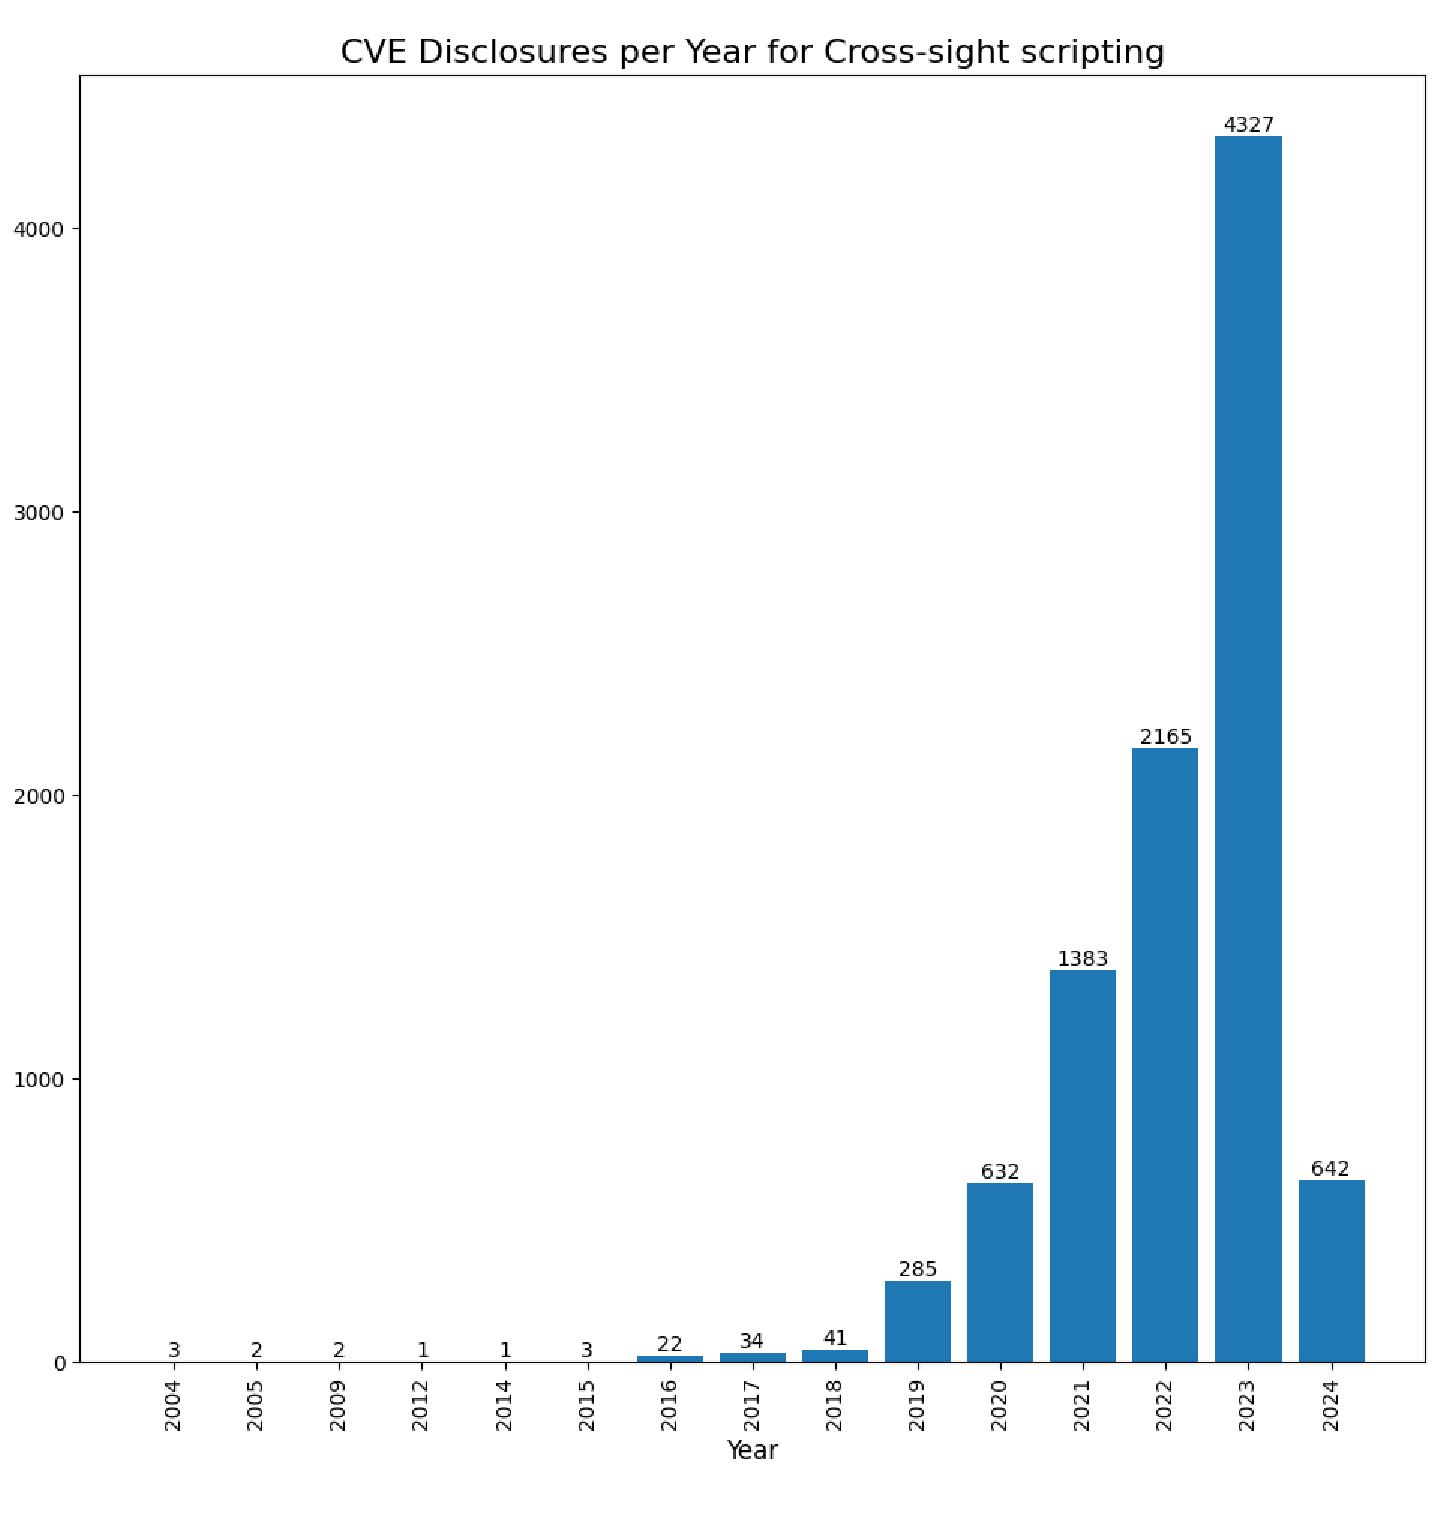
\includegraphics[width=0.8\textwidth]{figures/cross_site_per_year.pdf}
	\caption{\label{fig:cross_site_per_year}CVEs with descriptions containing at least five of the
		words from cluster four}
\end{figure}

\subsection{Latent Dirichlet Allocation Methodology}

The next approach to topic modeling utilizes Latent Dirichlet Allocation (LDA)~\cite{lda_origin} in
conjunction with Word2Vec~\cite{word2vec} embeddings to analyze Common Vulnerabilities and Exposures
(CVE) descriptions. As an unsupervised learning method, LDA is well-suited for exploring large
collections of text data without predefined categories~\cite{lda_origin, latent_handbook}. This is
particularly valuable in the CVE context, where we aim to discover latent themes in vulnerability
descriptions without prior knowledge of these themes. LDA's soft clustering approach allows CVE
descriptions to belong to multiple topics with varying probabilities~\cite{latent_handbook}, which is beneficial given
the multi-faceted nature of many vulnerabilities. Furthermore, LDA produces human-interpretable
topics~\cite{lda_origin}, facilitating easier derivation of insights from the clustering results.
The paper \say{Security trend analysis with CVE topic models, by Neuhaus \&
	Zimmerman(2010)}\cite{cve_topic_modelling} uses this technique to great effect on the NVD
dataset (the analysis was for data ending in 2009) giving precedence to LDA being effective for this
sort of task.

The methodology comprises several key steps:

\subsubsection{Data Preprocessing} I begin by preprocessing the CVE descriptions:

\begin{itemize}

	\item Custom stopwords are defined, combining standard English stopwords with domain-specific
	      terms (e.g., \say{vulnerability}, \say{attacker}).

	\item Each description is tokenized and filtered, removing stopwords and short tokens (length
	      $\leq 2$).

	\item A dictionary is created from the processed texts, filtering out extremely rare and
	      extremely common terms.

\end{itemize}

This data processing is necessary due to this type of topic discovery relying on word distributions,
and therefore word frequencies. As a result stop words just muddy the water and put more interesting
and relevant topic words further down.

\subsubsection{Word Embedding}

A Word2Vec~\cite{word2vec} model is trained on the preprocessed texts:

\begin{itemize} \item Vector size: 100 \item Window size: 5 \item Minimum word count: 2
\end{itemize}

This embedding captures semantic relationships between words in the CVE context.

The parameters chosen here just felt like reasonable defaults and have not been explored. There are
also other options in using something like pretrained fasttext~\cite{fasttext} as used in
\cite{nvd_clustering_fasttext}.

% \subsubsection*{Topic Coherence Metric}

% \todo[inline]{As I haven't really used these in a rigorous way, I am unsure if I should keep this
% 	in, I have not gone into detail on these as I feel like it may be wasted effort if I do not use them
% 	too much }

% I define a custom coherence metric based on Word2Vec similarities:

% \begin{equation}
% 	\mathit{Coherence} = \frac{\sum_{i=1}^{n}\sum_{j=i+1}^{n} \mathrm{similarity}(\mathit{word}_i, \mathit{word}_j)}{\binom{n}{2}}
% \end{equation}

% where $n$ is the number of top words in a topic (10 in my implementation).

% In addition I have kept track of the C-V coherence score used as default by Gensim, which comes from
% \cite{cv_coherence}

% \todo[inline]{Also have used perplexity, as a score as that was the common way in the original lda
% 	paper.... I haven't really used it though, just interesting in how unstable it was compared with the
% 	other coherence style metrics...}

\subsubsection{LDA Model Training}

I have done many different iterations of the models with varying numbers of topics and
hyperparameters. In grid search attempts I found that the different coherences metrics did not agree
with each other. In addition, as we are searching for unknown topics in a unsupervised fashion, it
is dubious how helpful these measures of fit are in any case. The hyperparameters below are broadly
matching what I found to be the best, however the main metric came from looking at the actual
clustering results, and the biggest impact came from the number of topics, with the final models
being picked by their purity score (as described in Section~\ref{sec:purity}) The key
hyperparameters used in the LDA model training are as follows:

\begin{itemize}

	\item Number of topics: {20, 40, 60, 80, 100}

	      \begin{itemize}

		      \item This parameter determines the number of topics the model attempts to discover in
		            the corpus.

		      \item The broad range allows for exploration of both coarse-grained and fine-grained
		            topic structures, which is crucial for identifying potential sub-categories within
		            CVSS metrics or broader themes across different metrics.

	      \end{itemize}

	\item $\alpha$: {\say{symmetric}}

	      \begin{itemize}

		      \item Controls the prior distribution over topic mixtures for each document.

		      \item The \say{symmetric} setting assumes all topics are equally likely a priori for each
		            document, providing an unbiased starting point for topic discovery in CVSS
		            vulnerability descriptions.

	      \end{itemize}

	\item $\eta$: {0.1}

	      \begin{itemize}

		      \item This is the prior for word distributions over topics.

		      \item The relatively small value of 0.1 can lead to more specific and distinct topics,
		            potentially helping in distinguishing between different CVSS categories more
		            clearly.

	      \end{itemize}

	\item Number of passes: {30}

	      \begin{itemize}

		      \item Represents the number of times the model cycles through the entire corpus during
		            training.

		      \item 30 passes allow the model to refine its topic assignments multiple times,
		            providing sufficient iterations to capture the underlying topic structure of CVSS
		            data without overfitting.

	      \end{itemize}

	\item Number of iterations: {200}

	      \begin{itemize}

		      \item Sets the maximum number of iterations for each document during the inference
		            process.

		      \item 200 iterations allow for thorough topic inference for each document, which is
		            particularly important for CVSS vulnerability descriptions that might contain
		            complex or technical language.

	      \end{itemize}

\end{itemize}

This set of hyperparameters collectively defines a thorough exploration of the topic space, allowing
for the discovery of both broad and specific themes in the CVSS data. The wide range of topic
numbers (20 to 100) was particularly impactful in identifying the optimal granularity for
representing the vulnerability descriptions. The LDA model is implemented using Gensim's
LdaMulticore\cite{gensim}, allowing for parallel processing. In general I found Gensim very nice to
work with, the model training was fast and the API made sense. The combination of Gensim's efficient
implementation and these carefully chosen hyperparameters facilitated a comprehensive exploration of
the topic structure in the CVSS vulnerability descriptions.

% \subsubsection{Model Evaluation and Selection}

% Models are evaluated based on the average topic coherence:

% \begin{equation}
% 	Score = \frac{1}{T}\sum_{t=1}^{T} Coherence(topic_t)
% \end{equation}

% where $T$ is the total number of topics.


\subsubsection{Topic Assignment and Analysis}

For each saved model:

\begin{itemize}

	\item Topic assignments are generated for each document in the corpus.

	\item Results, including document index, description, assigned topic, and CVSS data, are saved
	      in JSON format.

	\item The top 50 words for each topic are extracted and saved for interpretation.

\end{itemize}


\subsubsection{Cluster-Class Association}

For each class within each CVSS metric, we identify the most representative cluster:

\begin{itemize}

	\item Calculate the proportion of documents from each class assigned to each topic cluster.

	\item The cluster with the highest count for a given class is considered its best representative.

	\item Calculate the purity score for all the different numbers of topics

\end{itemize}

With the best cluster from a given set discovered, we now need to decided which number of clusters
provides the best overall fit. A rudimentary approach is to just use the purity score.

\subsection{Purity as a Cluster Evaluation Metric}\label{sec:purity}

Purity is a simple external evaluation measure for cluster quality, particularly useful when
predefined classes are available for the data~\cite{purity_usuage}.

\subsubsection{Definition and Calculation}

For a set of clusters $\Omega = \{\omega_1, \omega_2, ..., \omega_K\}$ and a set of classes $C =
	\{c_1, c_2, ..., c_J\}$, purity is defined as:

\begin{equation}
	\text{purity}(\Omega, C) = \frac{1}{N} \sum_{k=1}^K \max_j |\omega_k \cap c_j|
\end{equation}

where $N$ is the total number of objects, and $|\omega_k \cap c_j|$ is the number of objects in
cluster $\omega_k$ that belong to class $c_j$.

\subsubsection{Interpretation}

Purity ranges from 0 to 1, where 1 indicates perfect purity. A higher purity value generally
suggests better clustering quality with respect to the ground truth classes\cite{purity_info_ret}.

In the context of topic modeling for CVSS metrics, high purity would indicate that each discovered
topic strongly corresponds to a specific CVSS class.

\begin{figure}[h!]
	\centering

	\begin{minipage}[t]{\textwidth}
		\centering
		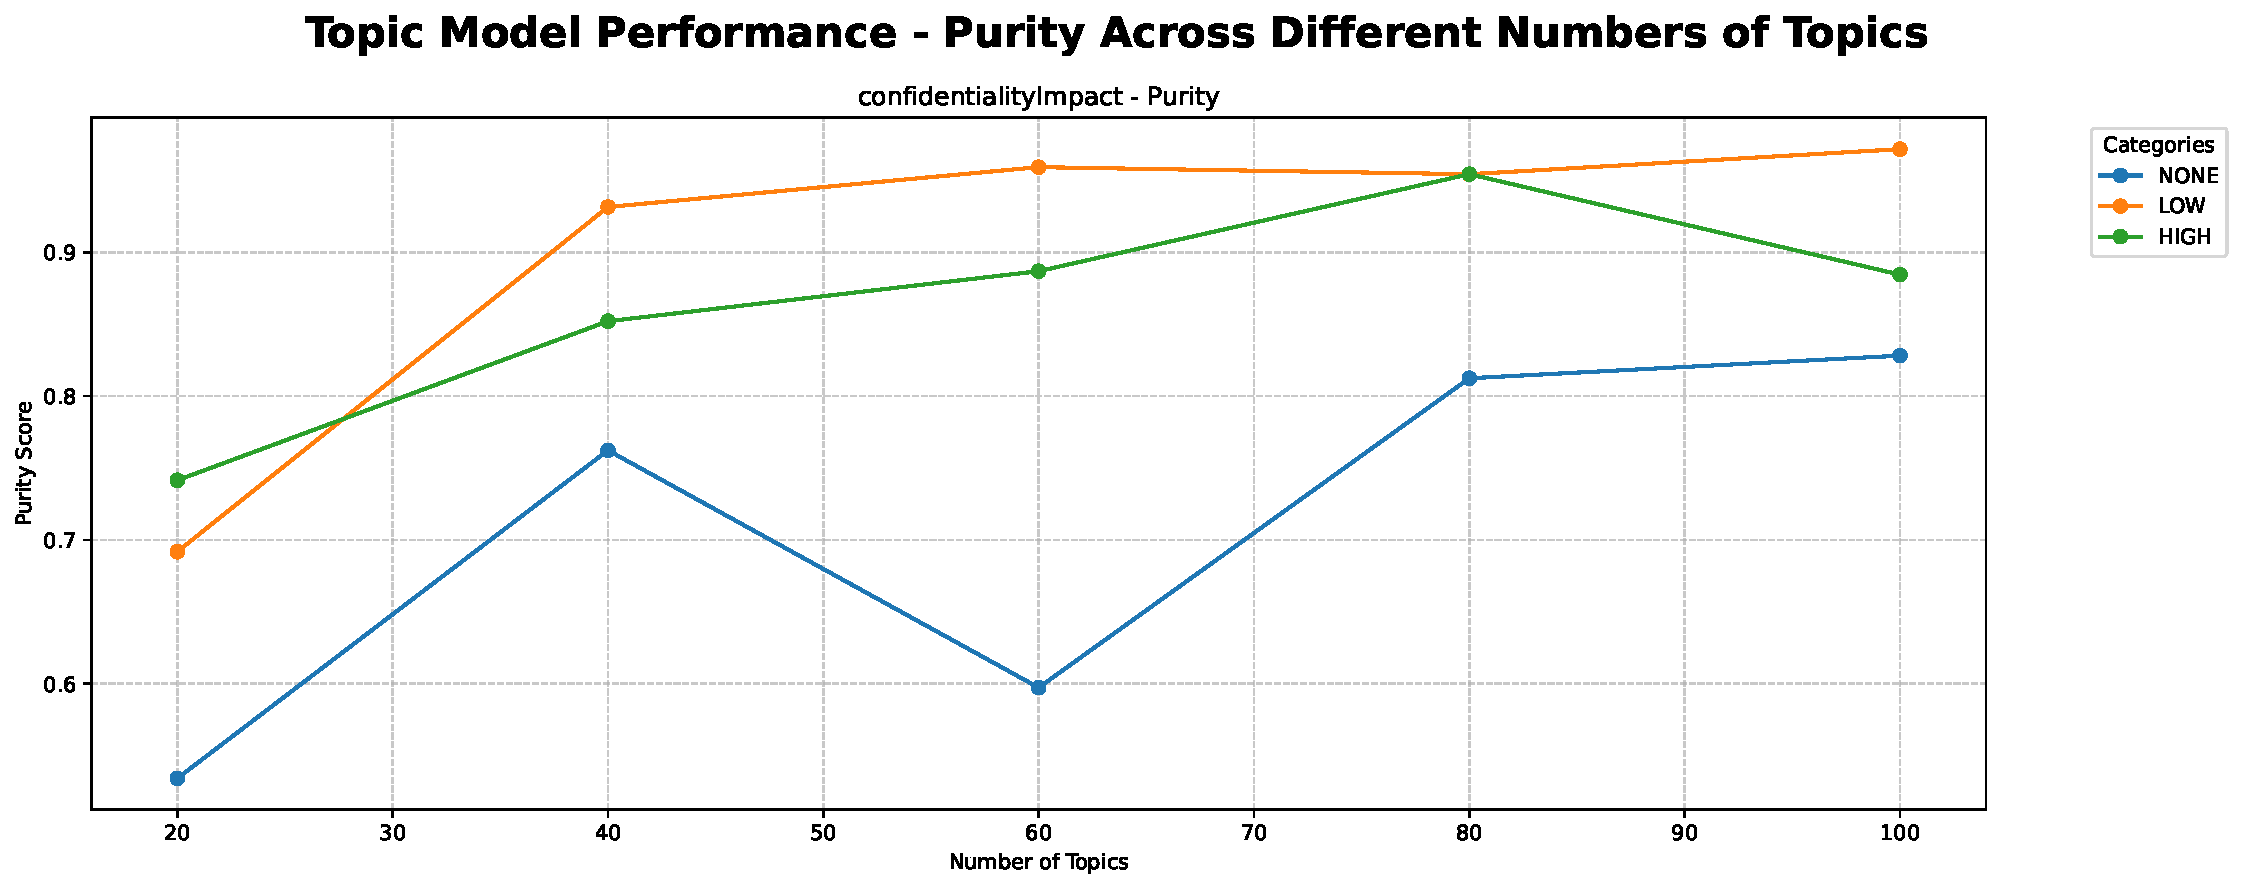
\includegraphics[width=0.8\textwidth]{figures/purity/topic_model_performance_purity_ground_truth_confidentialityImpact.pdf}
		\caption{The purity score for when the topics have been assigned with a focus on \texttt{Confidentiality Impact}, split by the different possible classes}
		\label{fig:purity_20_confidentiality}
	\end{minipage}

	\begin{minipage}[t]{\textwidth}
		\centering
		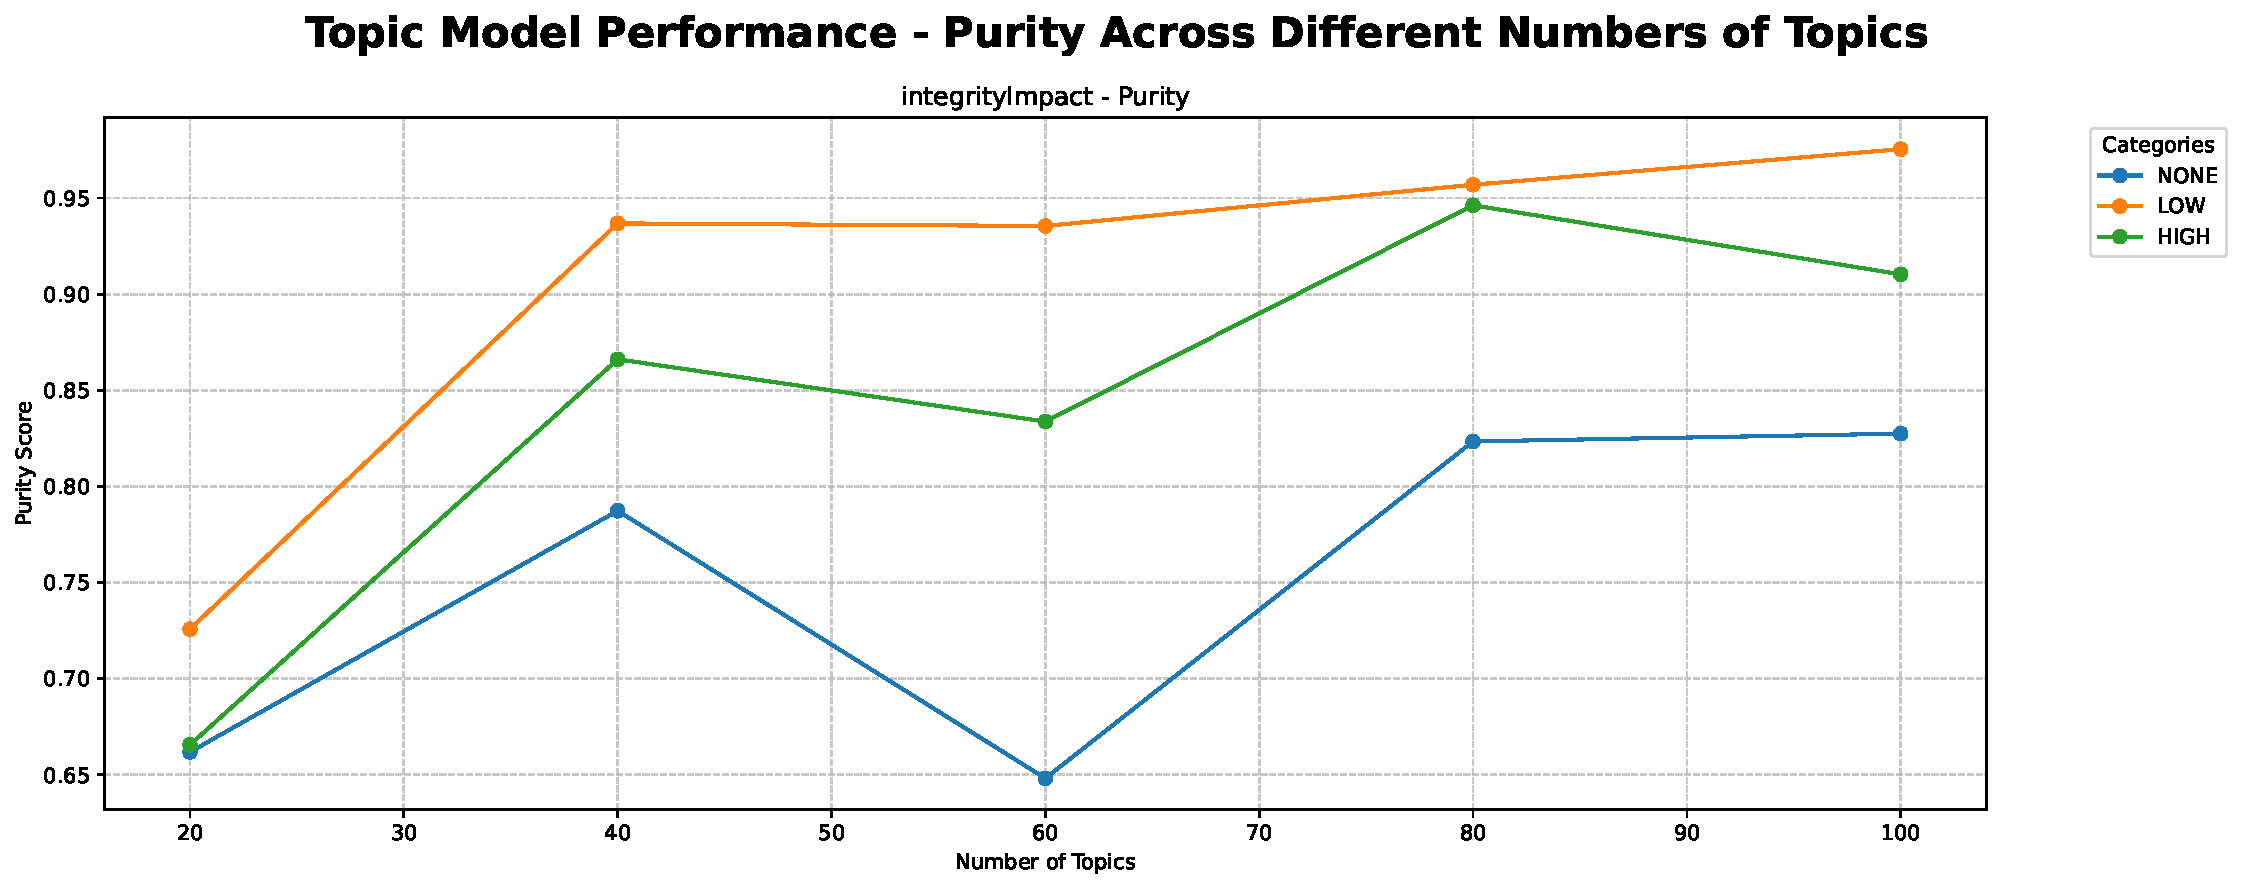
\includegraphics[width=0.8\textwidth]{figures/purity/topic_model_performance_purity_ground_truth_integrityImpact.pdf}
		\caption{The purity score for when the topics have been assigned with a focus on \texttt{Integrity Impact}, split by the different possible classes}
		\label{fig:purity_integrity}
	\end{minipage}


	\begin{minipage}[t]{\textwidth}
		\centering
		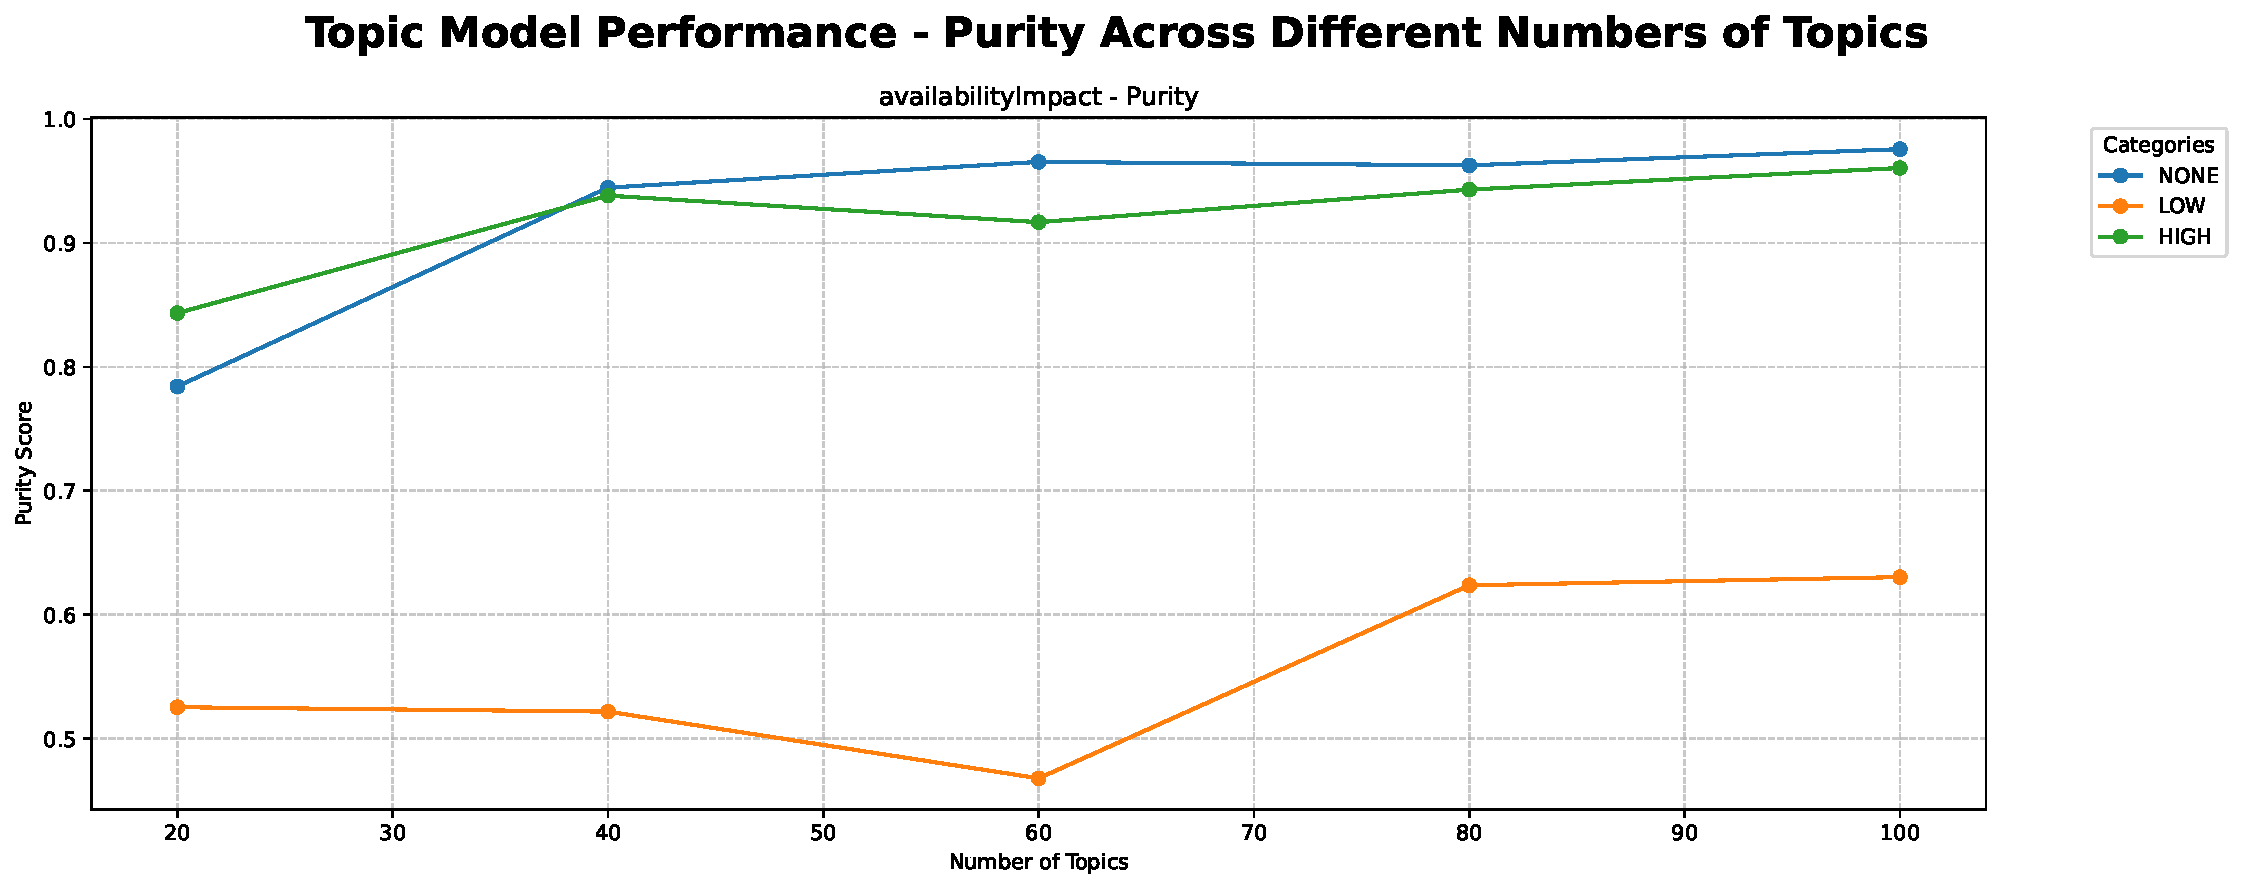
\includegraphics[width=0.8\textwidth]{figures/purity/topic_model_performance_purity_ground_truth_availabilityImpact.pdf}
		\caption{The purity score for when the topics have been assigned with a focus on \texttt{Availability Impact}, split by the different possible classes}
		\label{fig:purity_20_availability}
	\end{minipage}


\end{figure}

\subsubsection{Limitations}

It's important to note that purity tends to increase as the number of clusters increases, with a
trivial solution of perfect purity when each object is in its own cluster \cite{v-measure}.
Therefore, it should be interpreted cautiously, especially when comparing models with different
numbers of topics, however, as seen by Figures~\ref{fig:purity_20_confidentiality}, \ref{fig:purity_integrity},
\ref{fig:purity_20_availability}, this effect did not present
itself too strongly. This effect incentivise picking the number of topics around the elbow of the
graph (the point on a curve where the rate of change significantly shifts), as any minor increase in
the purity score could just be based on the inherent increase in the purity score as the number of
topics increase.





\subsection{Evaluation and Insights}

\subsubsection{Elephant in the Room, Data Imbalance}

As is obvious from Figure~\ref{fig:nvd_data}, the classes for each metric are highly imbalanced.
This is just a reality of the data and so is something to contend with. This aspect
made finding a well defined cluster for each topic difficult as well as making the graphing and
interpreting the outcome of the clustering somewhat awkward.

As an example, if we take look at Figure~\ref{fig:priviledgesRequired_BAD}, which shows the
clustering for \texttt{Privileges Required}  of the best cluster with a focus on the \texttt{HIGH} class, we
can see that even though we are trying to find the cluster with the best representation of
\texttt{HIGH} both of the other classes are more dominant. This is a result of the massive class
imbalance, the clustering cannot manage to find a class to represent such a little proportion of the
data. As a result the analysis will be focused on the metrics which are the most naturally balanced
as well as related to each other, these are the CIA triad, confidentiality, integrity, and availiability
impact.

% If we take a look at Figure~\ref{fig:integrityImpact_60_NONE_BAD}

\begin{figure}[h!]
	\centering
	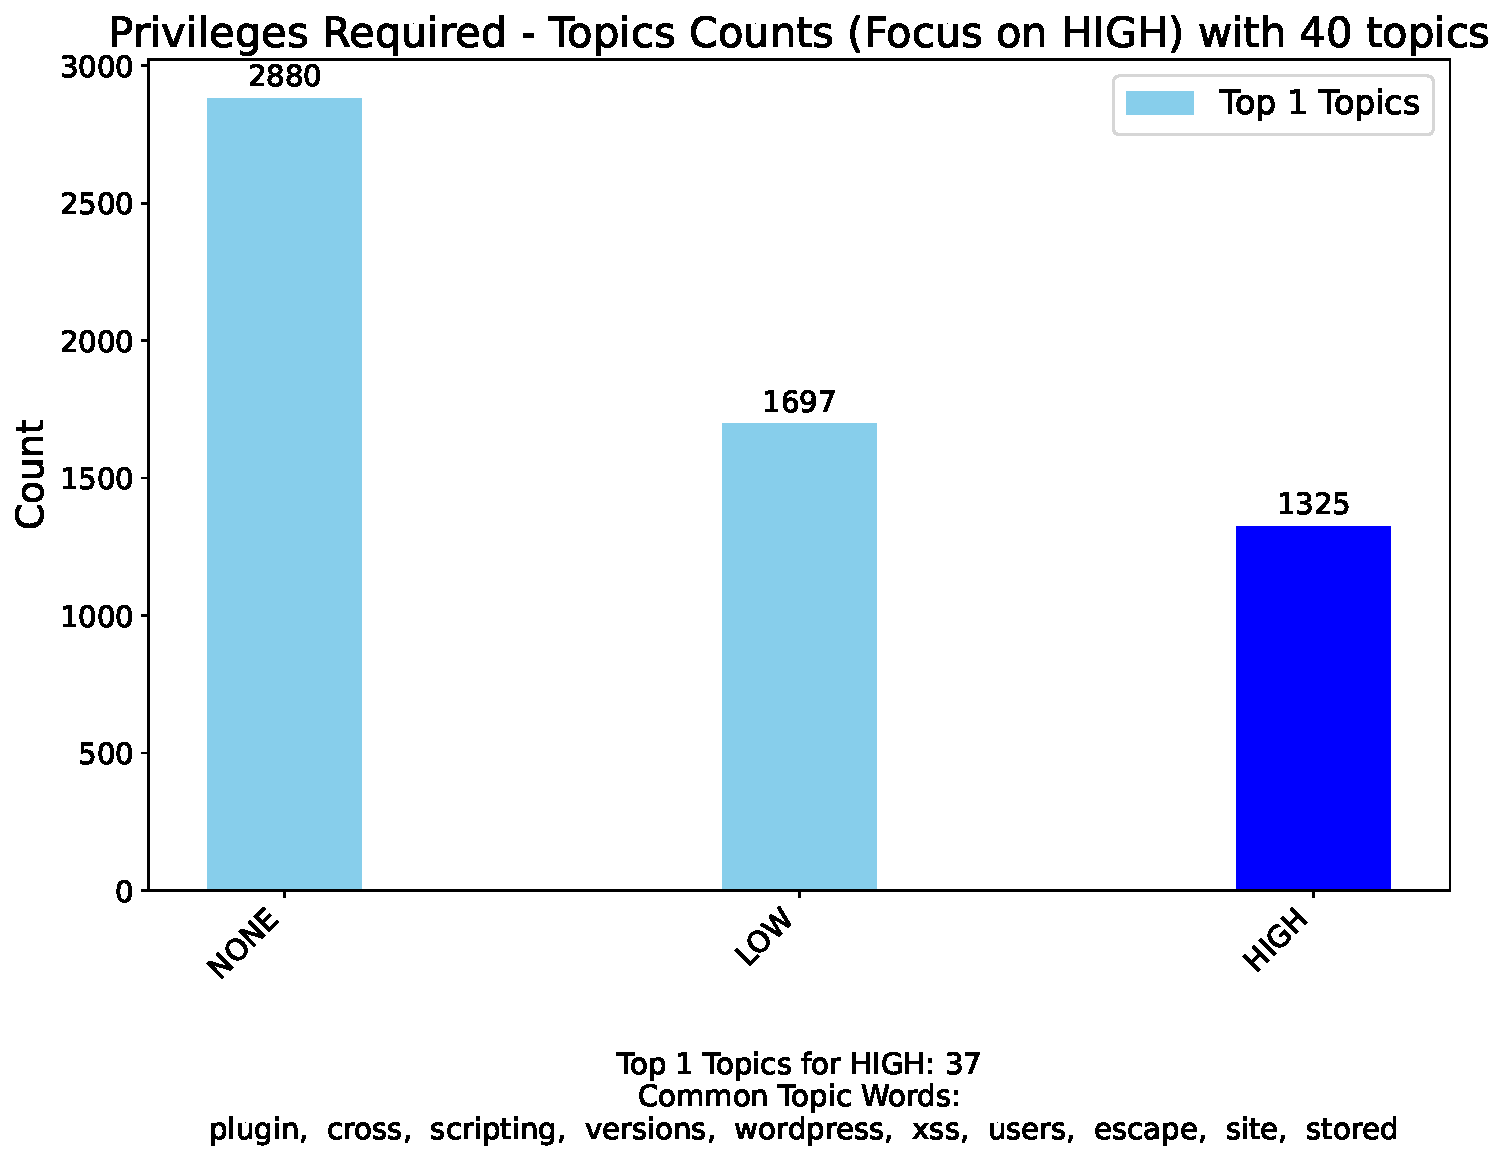
\includegraphics[width=0.7\textwidth]{figures/privilegesRequired/merged_top_k_topics_category_focus_counts_privilegesRequired_HIGH_k1.pdf}

	\caption{The counts of the documents within the best topic in relation to \texttt{Privileges Required} with
		target class \texttt{HIGH}}

	\label{fig:priviledgesRequired_BAD}
\end{figure}


% \begin{figure}[h!]

% 	\centering
% 	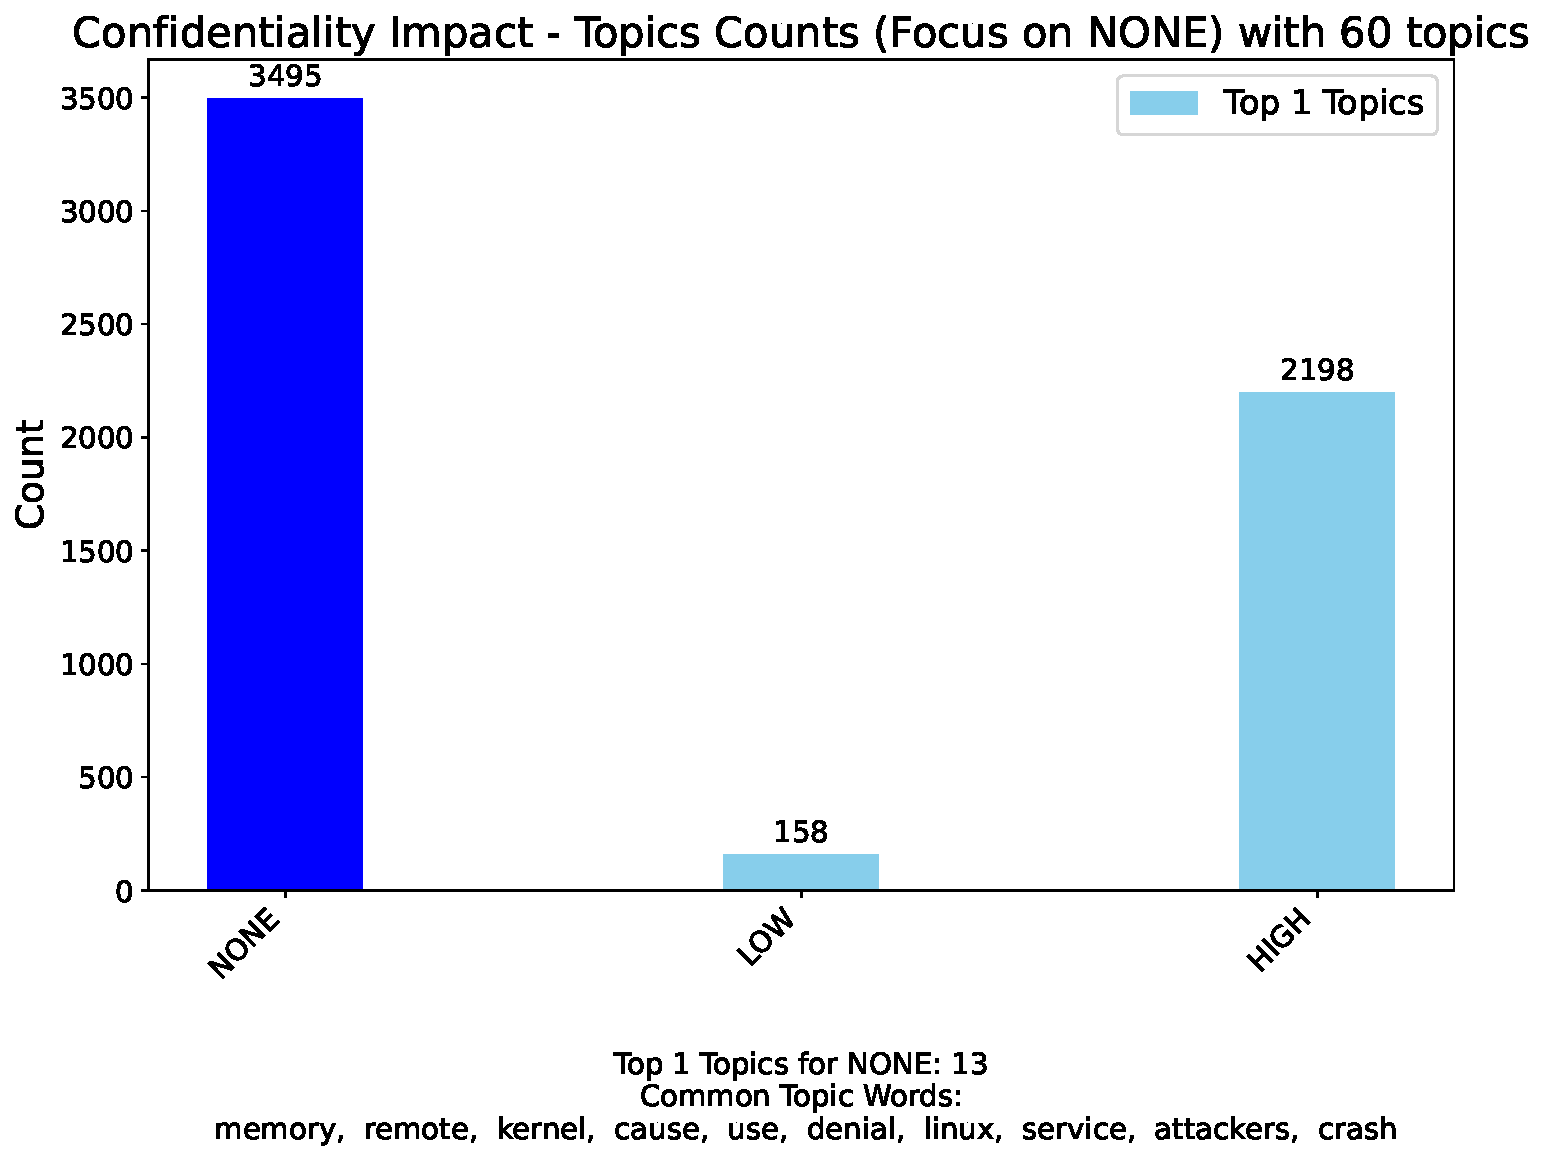
\includegraphics[width=0.8\textwidth]{figures/integrityImpact/integrityImpact_NONE_60_BAD.pdf}
% 	\caption{The counts of the documents within the best topic in relation to integrityImpact with
% 		target class \texttt{NONE}, for the number of clusters (60) with the lowest purity}
% 	\label{fig:integrityImpact_60_NONE_BAD}
% \end{figure}
\subsection{Clustering Results}

The clustering analysis using Latent Dirichlet Allocation (LDA) yielded insights into the patterns
of vulnerabilities as they relate to the Common Vulnerability Scoring System (CVSS) metrics,
particularly the integrity impact metric. While an ideal analysis would involve comparing our
clusters with the assigned Common Weakness Enumeration (CWE), the time constraints and the complex
nature of both our topic-based clusters and the CWE descriptions made automated cross-referencing
unfeasible for the time being.

\subsubsection{Methodology and Presentation}

The primary results of our analysis are presented in graphical form for each of the three CVSS
impact metrics: Integrity Impact, Confidentiality Impact, and Availability Impact. For each metric,
we provide three graphs corresponding to the three possible impact levels: \texttt{NONE},
\texttt{LOW}, and \texttt{HIGH}.

Each graph shows the distribution of documents across all three classes (\texttt{NONE},
\texttt{LOW}, \texttt{HIGH}) for the topic cluster that best represents the target class. This
approach allows us to visualize how effectively our clustering method separates vulnerabilities
based on their impact levels for each metric.

\subsubsection{Confidentiality Impact Analysis}

The \texttt{Confidentiality Impact} metric in CVSS measures the impact on confidentiality of a
successfully exploited vulnerability. Confidentiality refers to limiting information access and
disclosure to only authorized users, as well as preventing access by, or disclosure to, unauthorized
ones.

\begin{figure}[h!]
	\ContinuedFloat*
	\centering
	\begin{subfigure}{\textwidth}
		\centering
		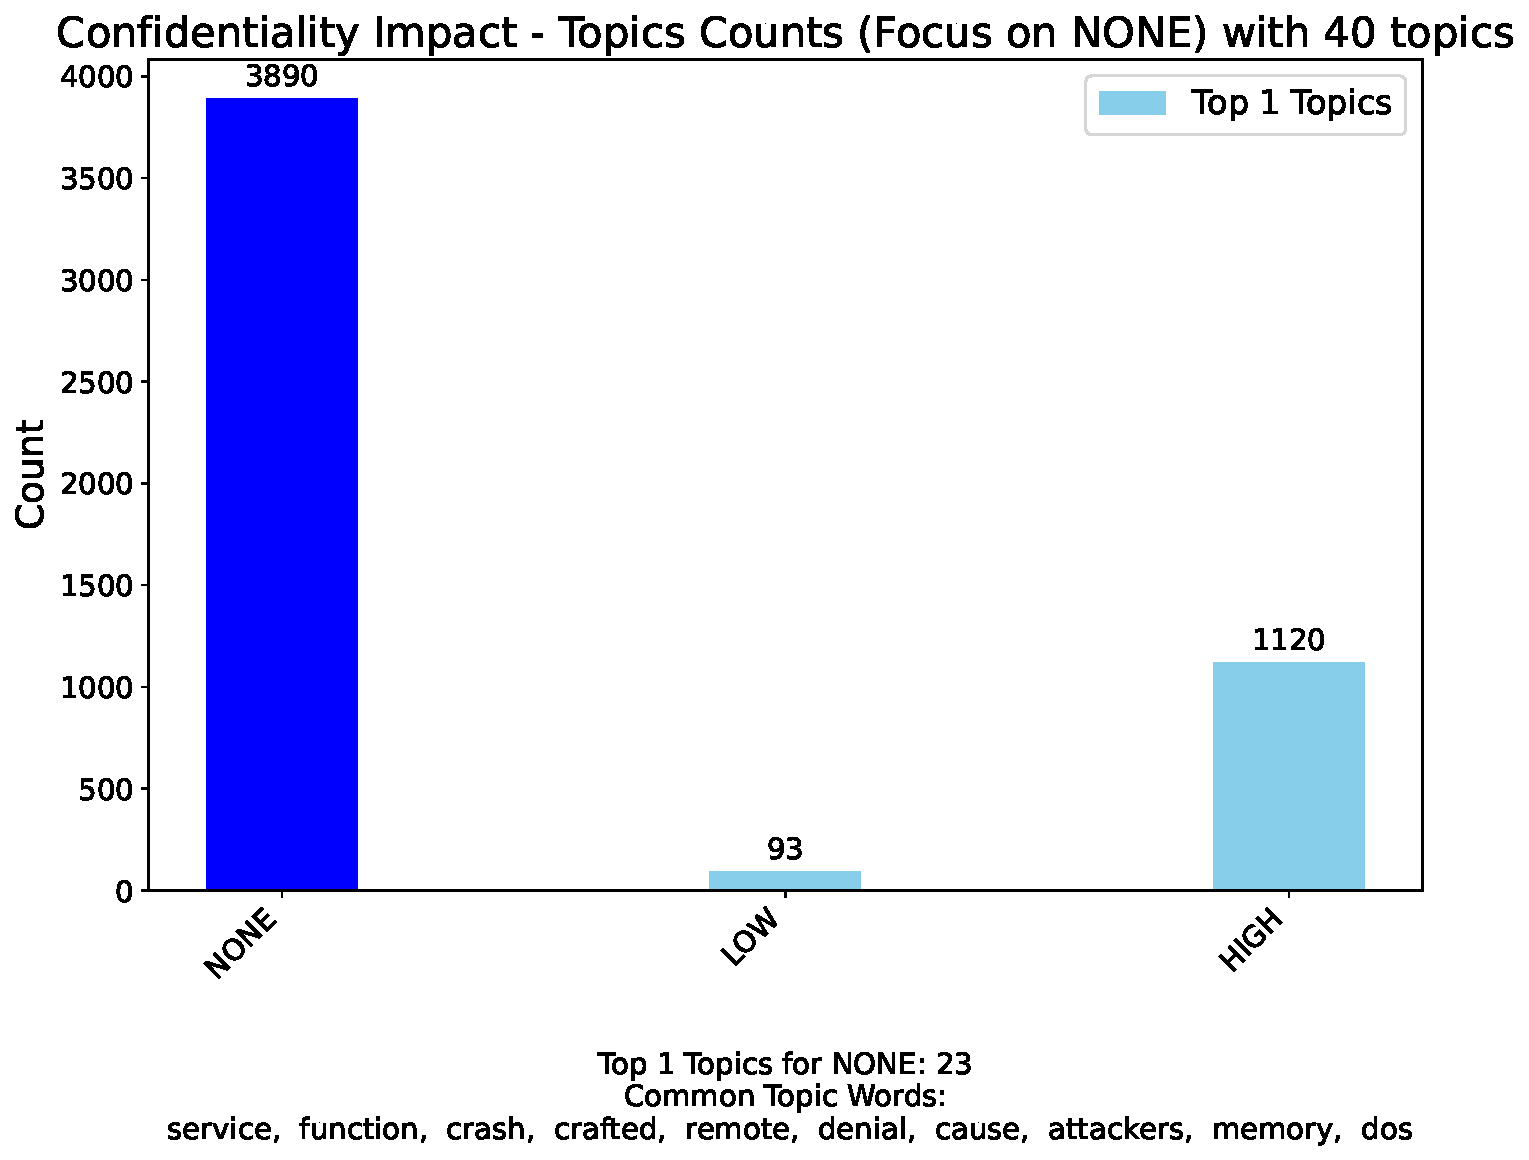
\includegraphics[width=0.7\textwidth]{figures/confidentialityImpact/merged_top_k_topics_category_focus_counts_confidentialityImpact_NONE_k1.pdf}
		\caption{The counts of the documents within the best topic in relation to \texttt{confidentiality Impact} with target class \texttt{NONE}}
		\label{fig:confidentialityImpact_60_NONE}
	\end{subfigure}

	\caption{Confidentiality Impact Topic Counts}
\end{figure}

\begin{figure}[h!]
	\ContinuedFloat
	\centering
	\begin{subfigure}{\textwidth}
		\centering
		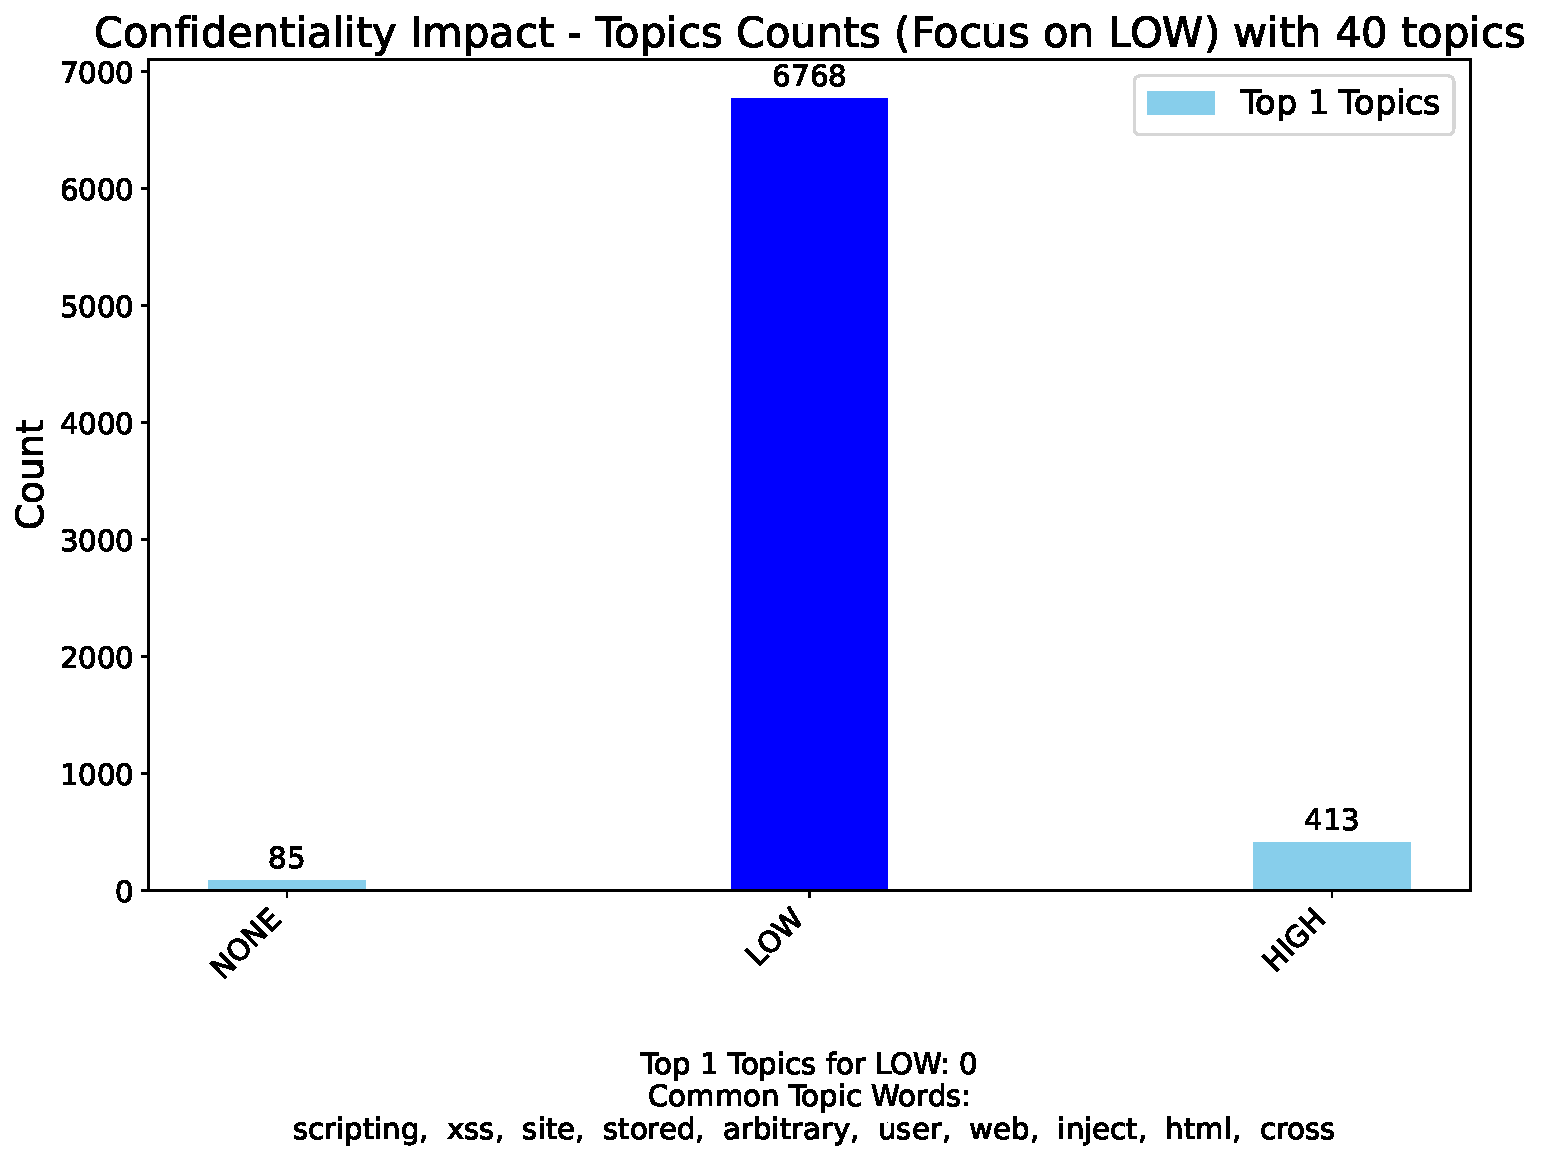
\includegraphics[width=0.7\textwidth]{figures/confidentialityImpact/merged_top_k_topics_category_focus_counts_confidentialityImpact_LOW_k1.pdf}
		\caption{The counts of the documents within the best topic in relation to \texttt{confidentiality Impact} with target class \texttt{LOW}}
		\label{fig:confidentialityImpact_60_LOW}
	\end{subfigure}

	\caption{Confidentiality Impact Topic Counts}
\end{figure}

\begin{figure}[h!]
	\ContinuedFloat
	\centering
	\begin{subfigure}{\textwidth}
		\centering
		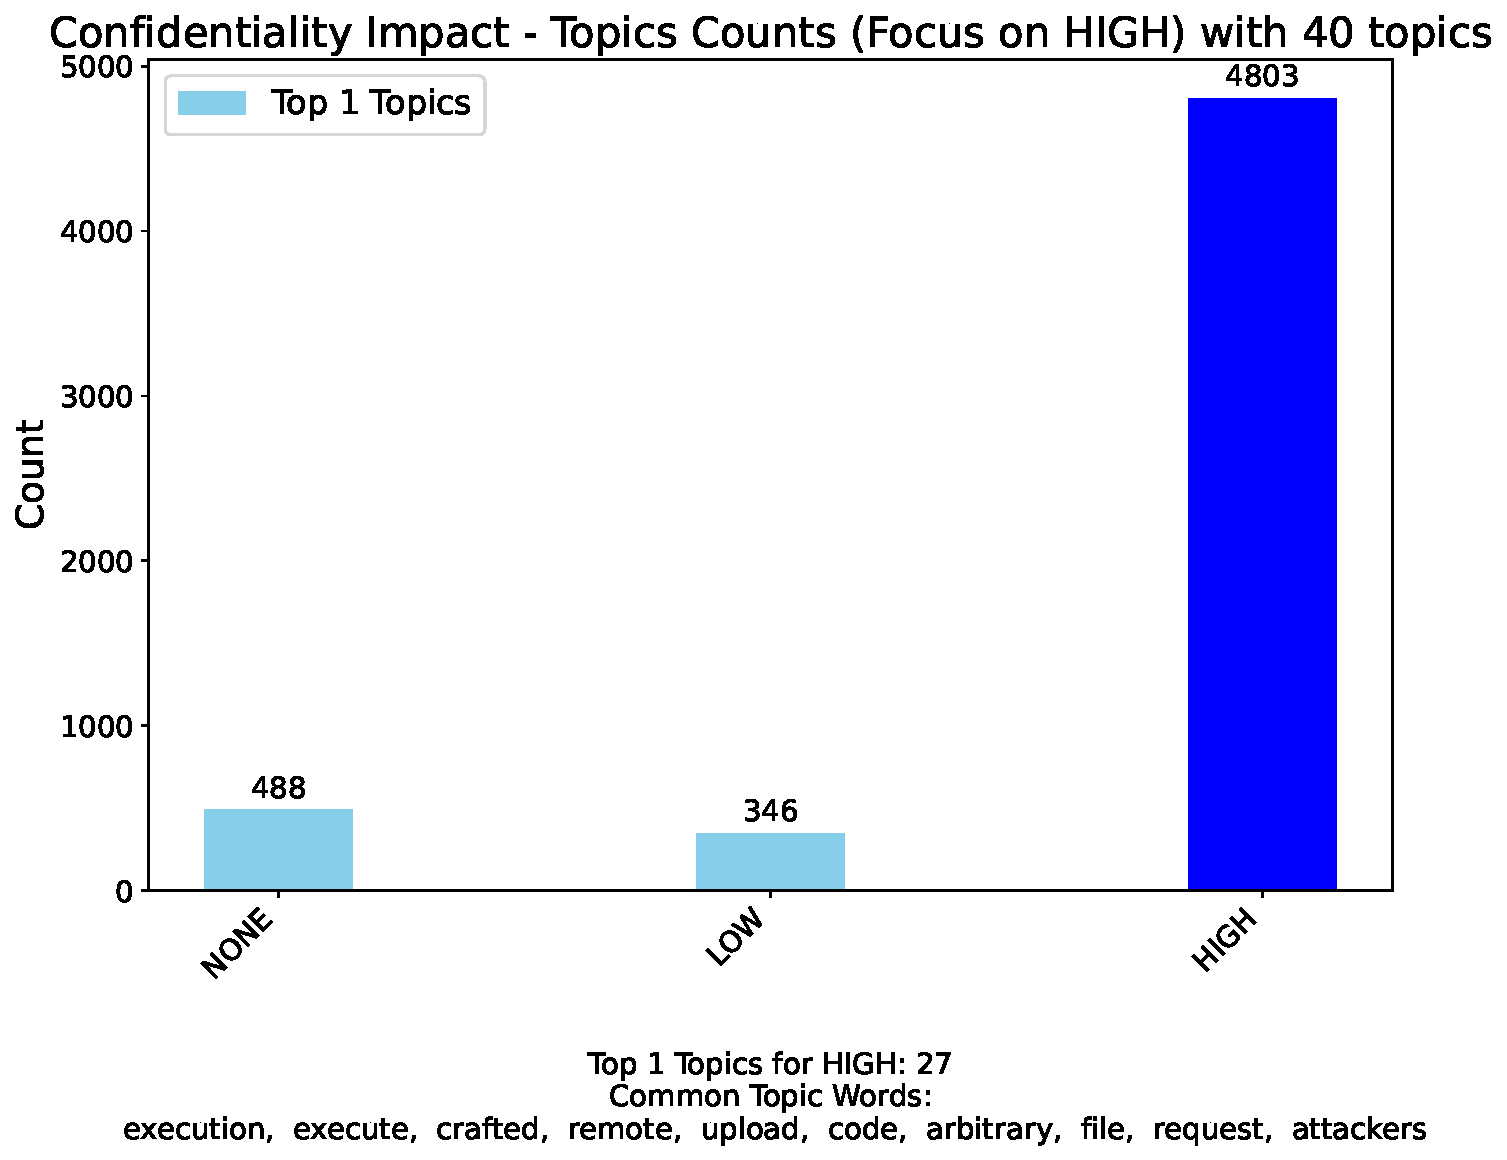
\includegraphics[width=0.7\textwidth]{figures/confidentialityImpact/merged_top_k_topics_category_focus_counts_confidentialityImpact_HIGH_k1.pdf}
		\caption{The counts of the documents within the best topic in relation to confidentialityImpact with target class \texttt{HIGH}}
		\label{fig:confidentialityImpact_60_HIGH}
	\end{subfigure}

	\caption{Confidentiality Impact Topic Counts}
\end{figure}

\subsubsection{Confidentiality Impact: Focus on class NONE}

Figure \ref{fig:confidentialityImpact_60_NONE} shows the distribution for the cluster best
representing the \texttt{NONE} class of confidentiality impact.

This cluster primarily contains vulnerabilities related to service disruptions and system crashes.
While these issues can severely affect system availability, they typically do not directly
compromise data confidentiality.

Key findings:

\begin{itemize}

	\item The cluster shows a clear majority of \texttt{NONE}-rated vulnerabilities.

	\item Predominant terms include \say{service}, \say{function}, \say{crash}, \say{crafted},
	      \say{remote}, \say{denial}, \say{cause}, \say{attackers}, \say{memory}, and \say{dos}.

	\item The presence of terms like \say{denial} and \say{dos} (denial of service) aligns with
	      vulnerabilities that affect system availability rather than confidentiality.

	\item This cluster effectively identifies vulnerabilities with no direct impact on
	      confidentiality.

\end{itemize}

\subsubsection{Confidentiality Impact: Focus on class LOW}

Figure \ref{fig:confidentialityImpact_60_LOW} represents the distribution for the cluster best
representing the \texttt{LOW} class of confidentiality impact. This cluster predominantly
features web-based vulnerabilities, particularly cross-site scripting (XSS) attacks. These types of
vulnerabilities can indeed cause confidentiality issues, but they are usually limited in scope,
typically affecting individual user sessions rather than compromising the entire system's
confidentiality.

Key findings:

\begin{itemize}

	\item The cluster shows a majority of \texttt{LOW}-rated vulnerabilities, with some overlap into
	      other categories.

	\item Predominant terms include \say{scripting}, \say{xss}, \say{site}, \say{stored}, \say{arbitrary}, \say{user},
	      \say{web}, \say{inject}, \say{html}, and \say{css}.

	\item The prevalence of web-related terms suggests that this cluster captures client-side
	      vulnerabilities that often have a lower impact on overall system confidentiality.

	\item This cluster aligns with expectations for low-impact confidentiality issues in web
	      applications.

\end{itemize}

\subsubsection{Confidentiality Impact: Focus on class LOW}

Figure \ref{fig:confidentialityImpact_60_HIGH} shows the distribution for the cluster best
representing the \texttt{HIGH} class of confidentiality impact. In this cluster, we see a focus
on remote code execution and file manipulation vulnerabilities. These types of attacks have the
potential to severely compromise data confidentiality by allowing unauthorized access to sensitive
information or system resources. Key findings:

\begin{itemize}

	\item The cluster shows a strong representation of \texttt{HIGH}-rated vulnerabilities.

	\item Predominant terms include \say{execution}, \say{execute}, \say{crafted},
	      \say{remote}, \say{upload}, \say{code},
	      \say{arbitrary}, \say{file}, \say{request}, and \say{attackers}.

	\item The presence of terms like \say{remote} and \say{arbitrary} suggests vulnerabilities that allow
	      attackers to gain extensive access to a system, potentially compromising large amounts of
	      confidential data.

	\item This cluster effectively captures severe confidentiality breaches that align with
	      cybersecurity expert expectations for high-impact confidentiality issues.

\end{itemize}

The analysis of these clusters for Confidentiality Impact reveals clear distinctions between the
NONE, LOW, and HIGH categories. The clustering effectively separates vulnerabilities based on their
potential to compromise data confidentiality, from those with no impact (like denial of service
attacks) to severe breaches (such as remote code execution). This demonstrates the model's ability
to capture the nuances of confidentiality impacts in various types of vulnerabilities.

\subsubsection{Integrity Impact Analysis}

The \texttt{Integrity Impact} metric in CVSS refers to the degree to which a vulnerability, if exploited,
could affect the trustworthiness and veracity of data. A high integrity impact implies that data
could be significantly corrupted or altered, potentially leading to serious consequences for the
affected system or its users.

\begin{figure}[h!]
	\ContinuedFloat*
	\centering
	\begin{subfigure}{\textwidth}
		\centering
		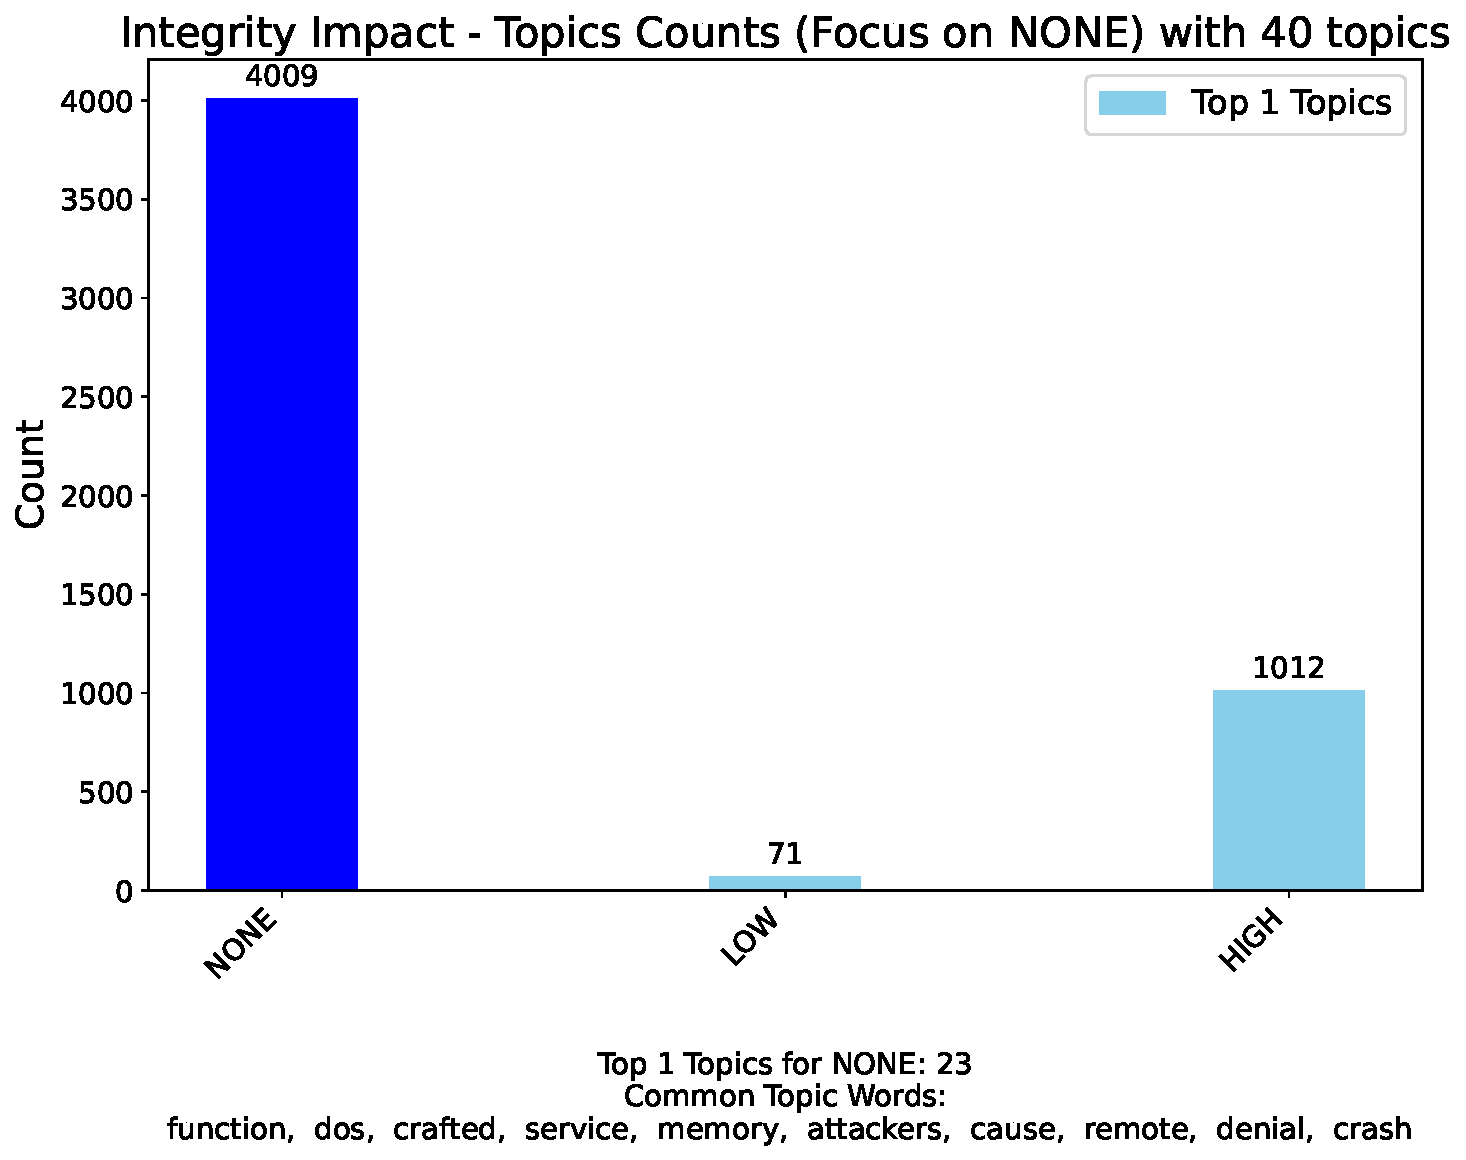
\includegraphics[width=0.7\textwidth]{figures/integrityImpact/merged_top_k_topics_category_focus_counts_integrityImpact_NONE_k1.pdf}
		\caption{The counts of the documents within the best topic in relation to \texttt{Integrity
				Impact} with
			target class \texttt{NONE}}

		\label{fig:integrityImpact_60_NONE}
	\end{subfigure}
	\caption{Integrity Impact Topic Counts}

\end{figure}

\begin{figure}[h!]
	\ContinuedFloat
	\centering
	\begin{subfigure}{\textwidth}
		\centering
		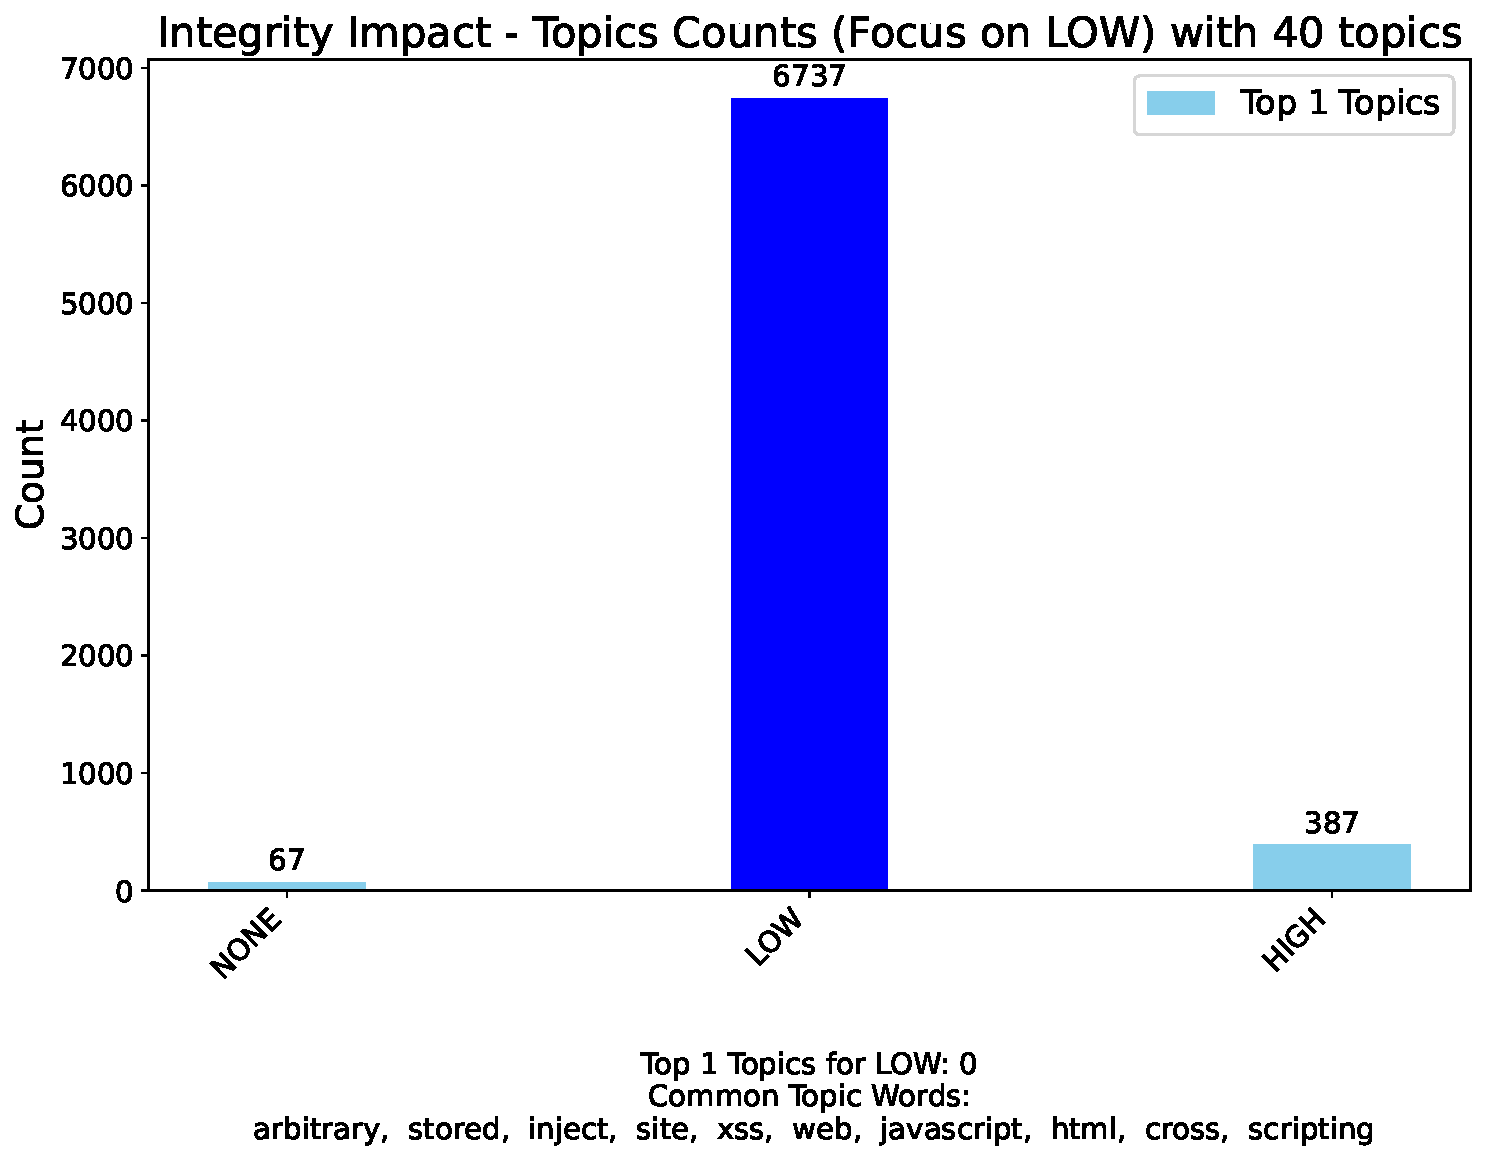
\includegraphics[width=0.7\textwidth]{figures/integrityImpact/merged_top_k_topics_category_focus_counts_integrityImpact_LOW_k1.pdf}
		\caption{The counts of the documents within the best topic in relation to \texttt{Integrity Impact} with target class \texttt{LOW}}
		\label{fig:integrityImpact_60_LOW}
	\end{subfigure}

	\caption{Integrity Impact Topic Counts}
\end{figure}

\begin{figure}[h!]
	\ContinuedFloat
	\centering
	\begin{subfigure}{\textwidth}
		\centering
		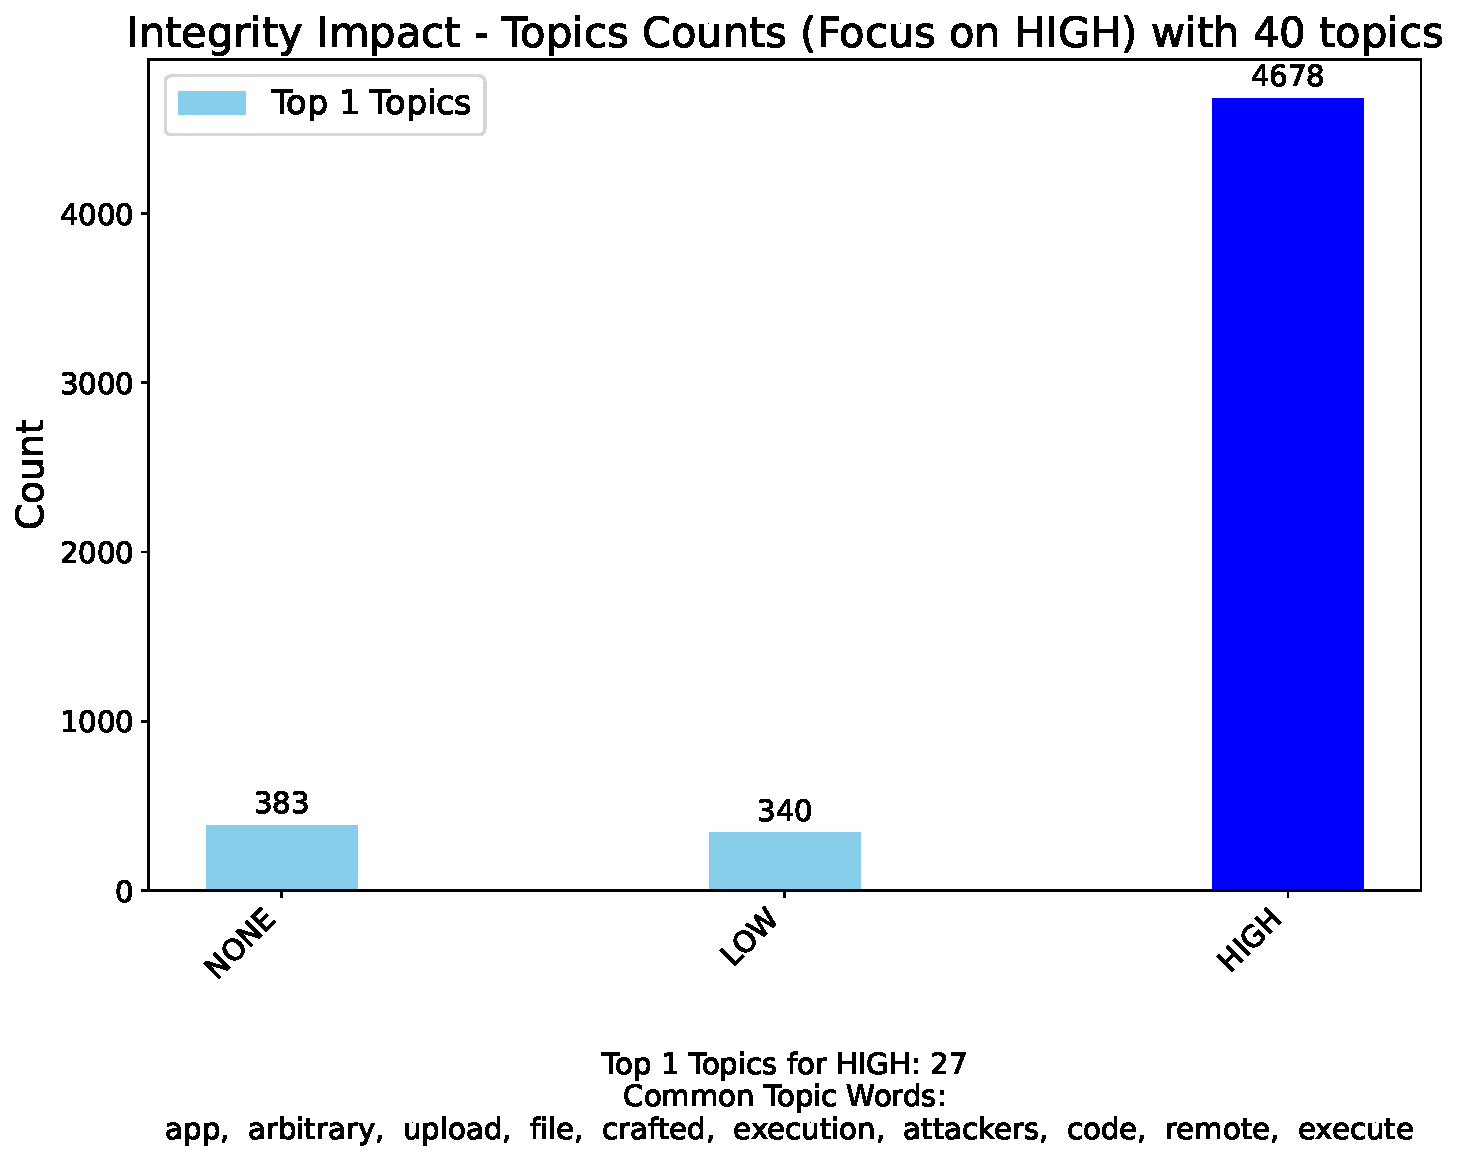
\includegraphics[width=0.7\textwidth]{figures/integrityImpact/merged_top_k_topics_category_focus_counts_integrityImpact_HIGH_k1.pdf}
		\caption{The counts of the documents within the best topic in relation to integrityImpact with target class \texttt{HIGH}}
		\label{fig:integrityImpact_60_HIGH}
	\end{subfigure}

	\caption{Integrity Impact Topic Counts}
\end{figure}

\subsubsection{Integrity Impact: Focus on class NONE}

Figure \ref{fig:integrityImpact_60_NONE} shows the distribution for the cluster best representing
the \texttt{NONE} class of integrity impact.


In this cluster, we observe a predominance of vulnerabilities related to denial of service attacks
and system crashes. While these issues are serious and can affect system availability, they
typically do not directly compromise data integrity. This aligns with the expectations for
vulnerabilities classified as having no integrity impact.

Key findings:
\begin{itemize}

	\item The cluster shows a clear majority of \texttt{NONE}-rated vulnerabilities.

	\item Common terms in this cluster likely include \say{denial of service}, \say{crash}, and
	      \say{dos}.

	\item This result supports the effectiveness of our clustering in identifying vulnerabilities
	      with no integrity impact.

\end{itemize}

\subsubsection{Integrity Impact: Focus on class LOW}

Figure \ref{fig:integrityImpact_60_LOW} represents the distribution for the cluster best
representing the \texttt{LOW} class of integrity impact.

This cluster predominantly features cross-site scripting (XSS) vulnerabilities and other generally
web browser based attacks. These types of vulnerabilities can indeed cause data integrity issues, but
they are usually limited in scope, typically affecting individual user interactions rather than
compromising the entire application's data integrity.

Key findings:
\begin{itemize}

	\item The cluster shows a majority of \texttt{LOW}-rated vulnerabilities, with some overlap into
	      other categories.

	\item Common terms likely include \say{cross-site scripting}, \say{XSS}, \say{javascript}, and \say{html}.

	\item This cluster aligns with our earlier k-means clustering results, providing some
	      similarities between the clustering
\end{itemize}

\subsubsection{Integrity Impact: Focus on class HIGH}

Figure \ref{fig:integrityImpact_60_HIGH} shows the distribution for the cluster best representing
the \texttt{HIGH} class of integrity impact.


In this cluster, we see a focus on remote code execution vulnerabilities. These
types of attacks have the potential to severely compromise data integrity by allowing unauthorized
modification or corruption of server contents.

Key findings:
\begin{itemize}

	\item The cluster shows a strong representation of \texttt{HIGH}-rated vulnerabilities.

	\item Common terms likely include \say{remote}, \say{execution}

	\item The prevalence of these severe vulnerabilities in this cluster aligns with cybersecurity
	      expert expectations for high-impact integrity issues.

\end{itemize}

\subsubsection{Availability Impact Analysis}

The \texttt{Availability Impact} metric in CVSS measures the impact on the availability of the
affected component resulting from a successfully exploited vulnerability. This metric refers to the
loss of availability of the impacted component itself, such as a networked service (e.g., web,
database, email).

\begin{figure}[h!]
	\ContinuedFloat*
	\centering
	\begin{subfigure}{\textwidth}
		\centering
		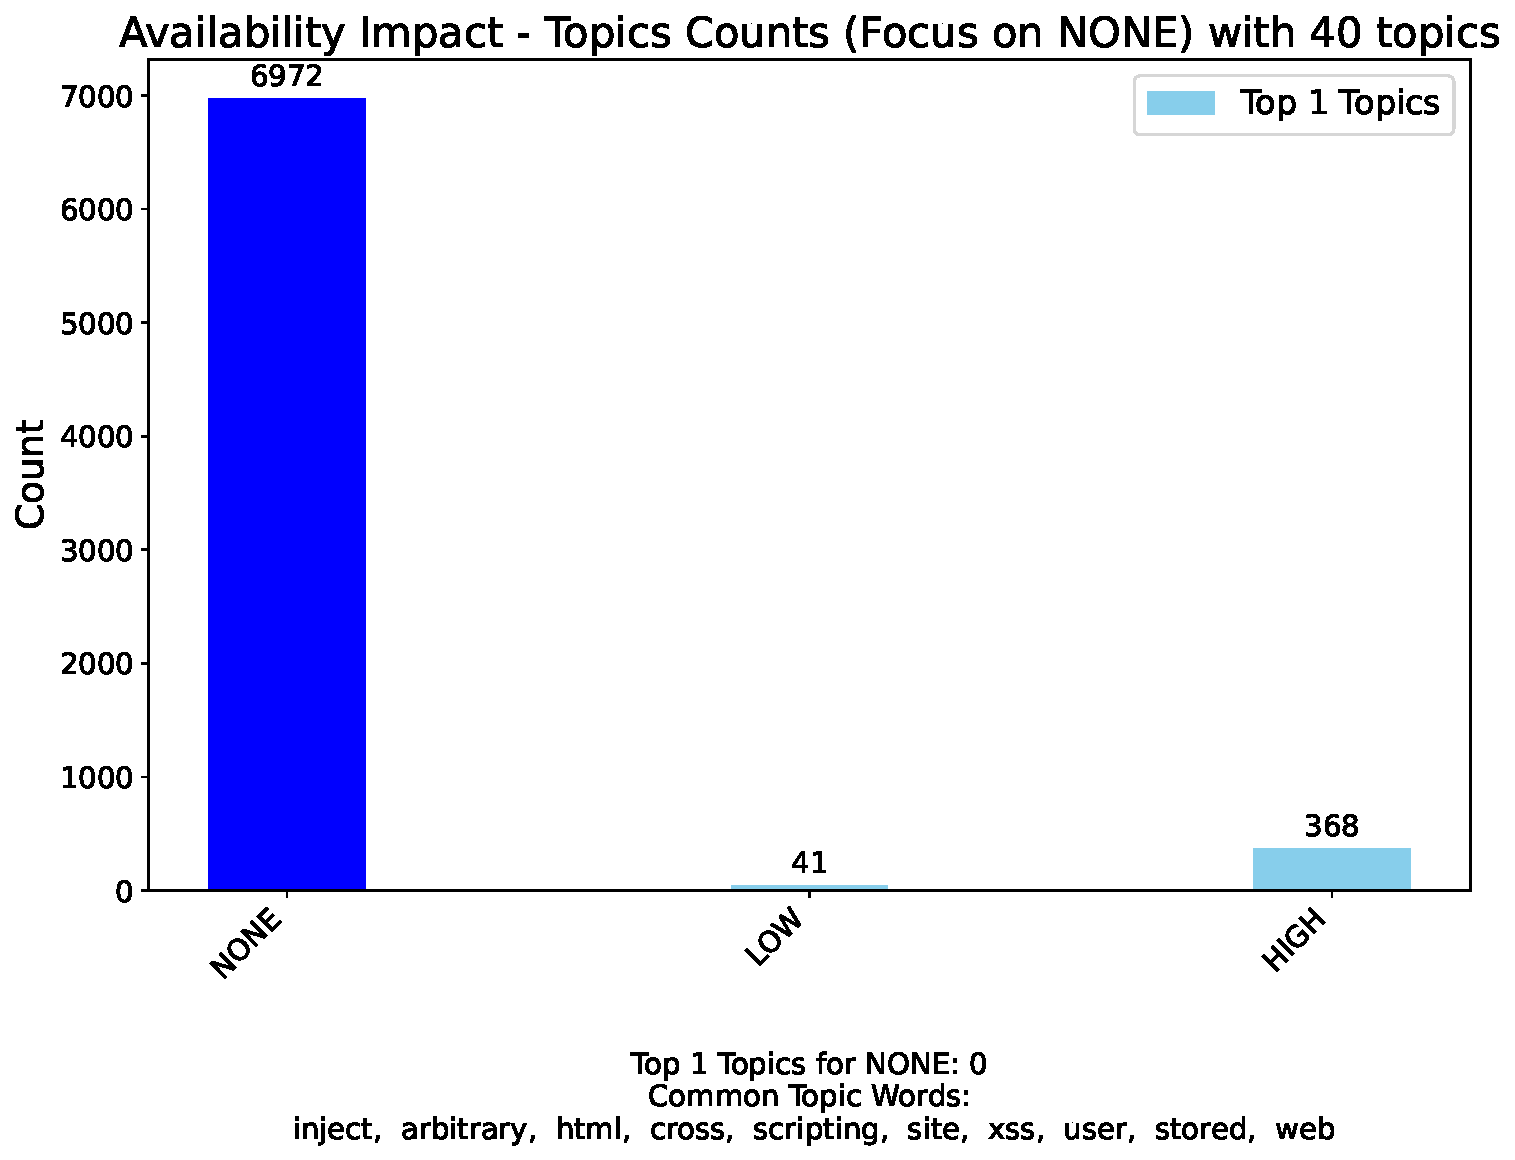
\includegraphics[width=0.7\textwidth]{figures/availabilityImpact/merged_top_k_topics_category_focus_counts_availabilityImpact_NONE_k1.pdf}

		\caption{The counts of the documents within the best topic in relation to \texttt{availability
				Impact} with
			target class \texttt{NONE}}
	\end{subfigure}


	\caption{Availability Impact Topic Counts}
	\label{fig:availabilityImpact_60_NONE}
\end{figure}

\begin{figure}[h!]
	\ContinuedFloat
	\centering
	\begin{subfigure}{\textwidth}
		\centering
		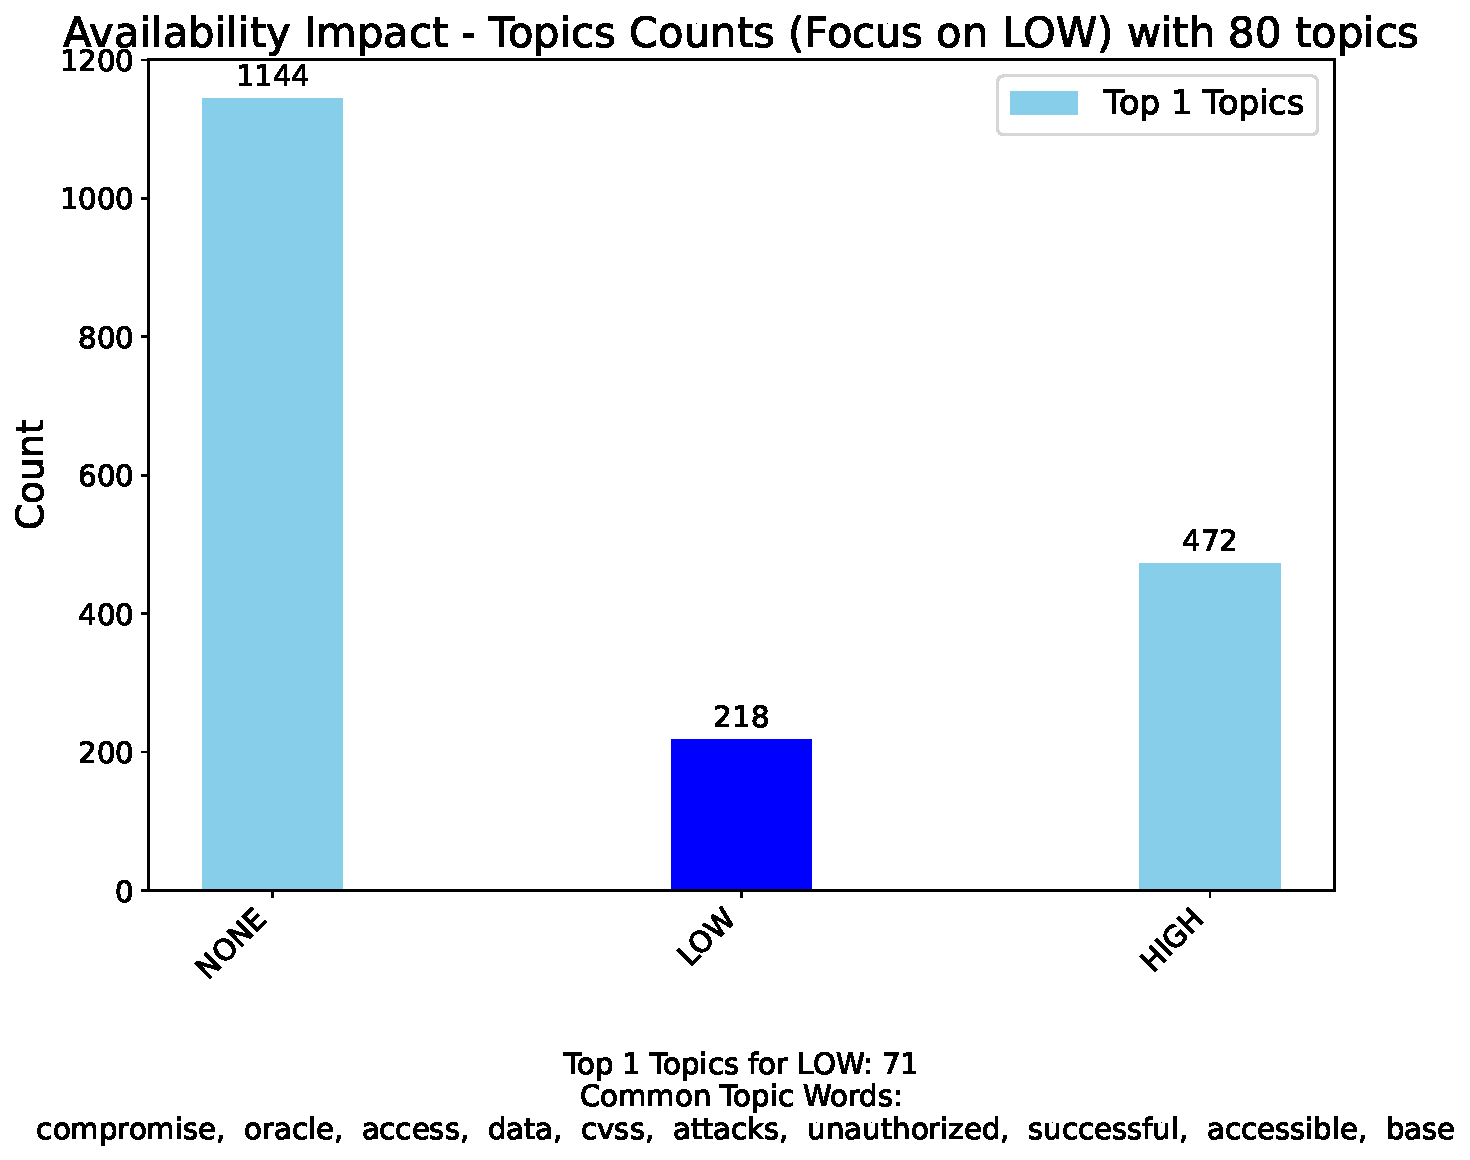
\includegraphics[width=0.7\textwidth]{figures/availabilityImpact/merged_top_k_topics_category_focus_counts_availabilityImpact_LOW_k1.pdf}
		\caption{The counts of the documents within the best topic in relation to \texttt{availability Impact} with target class \texttt{LOW}}
		\label{fig:availabilityImpact_60_LOW}
	\end{subfigure}

	\caption{Availability Impact Topic Counts}
\end{figure}

\begin{figure}[h!]
	\ContinuedFloat
	\centering
	\begin{subfigure}{\textwidth}
		\centering
		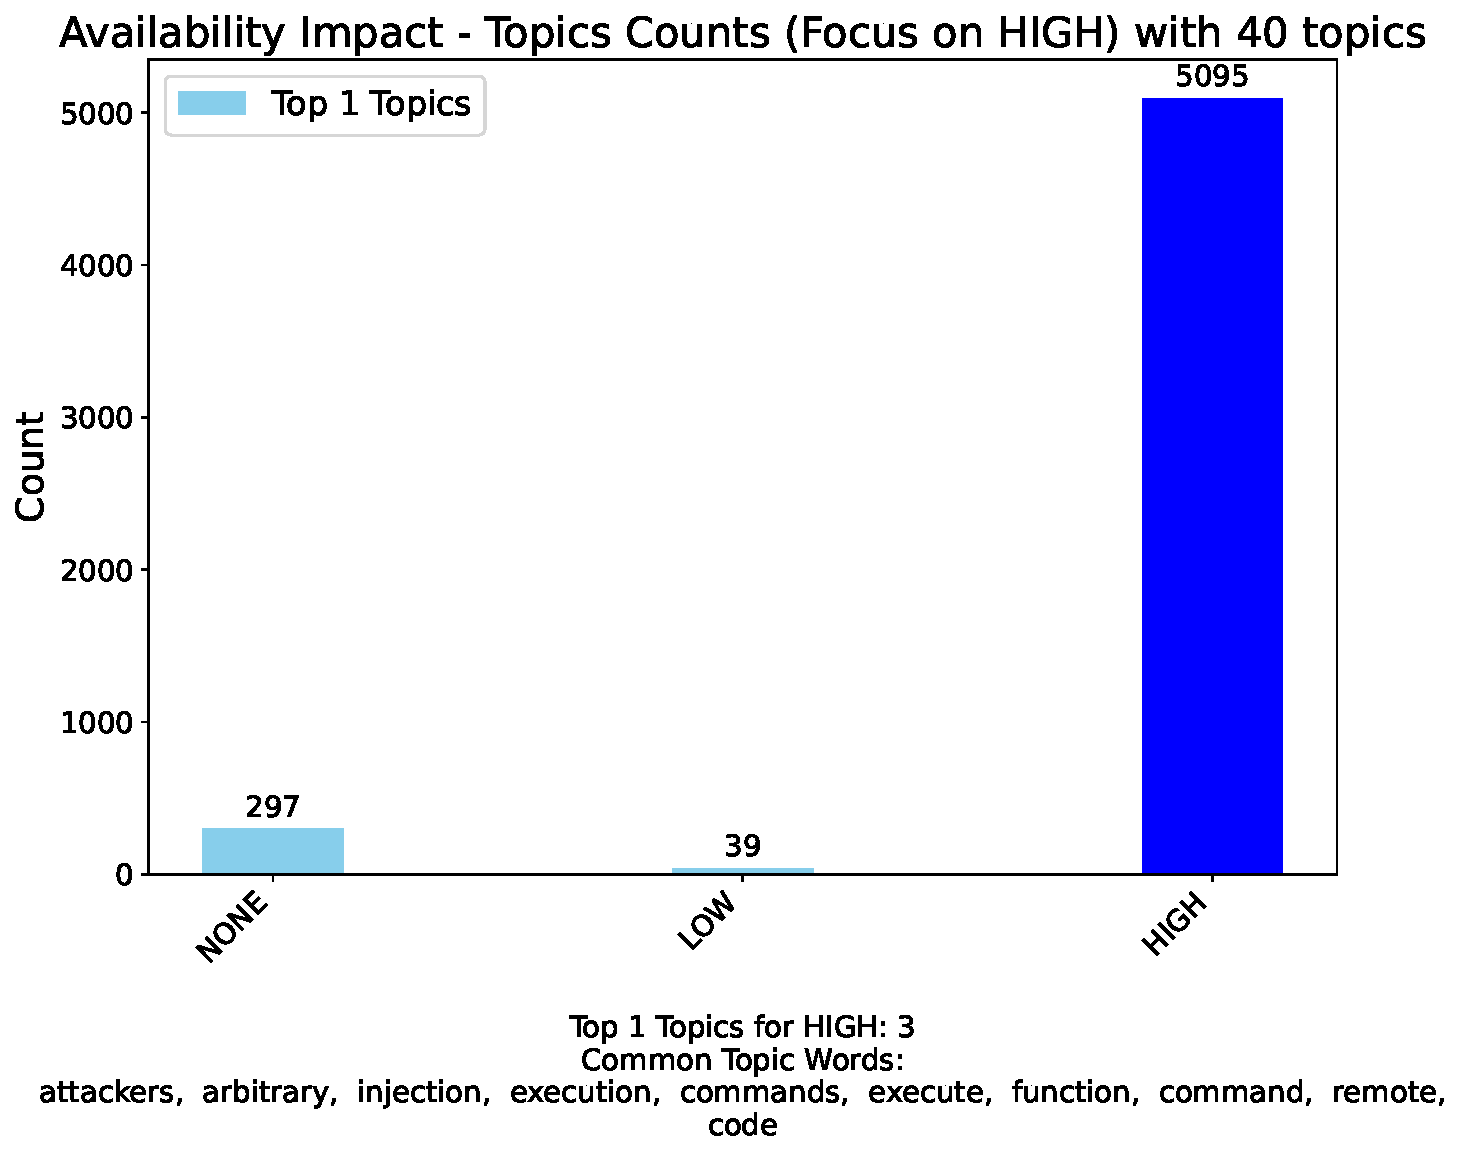
\includegraphics[width=0.7\textwidth]{figures/availabilityImpact/merged_top_k_topics_category_focus_counts_availabilityImpact_HIGH_k1.pdf}
		\caption{The counts of the documents within the best topic in relation to availabilityImpact with target class \texttt{HIGH}}
		\label{fig:availabilityImpact_60_HIGH}
	\end{subfigure}

	\caption{Availability Impact Topic Counts}
\end{figure}

\begin{figure}[h!]
	\ContinuedFloat
	\begin{subfigure}{\textwidth}
		\centering
		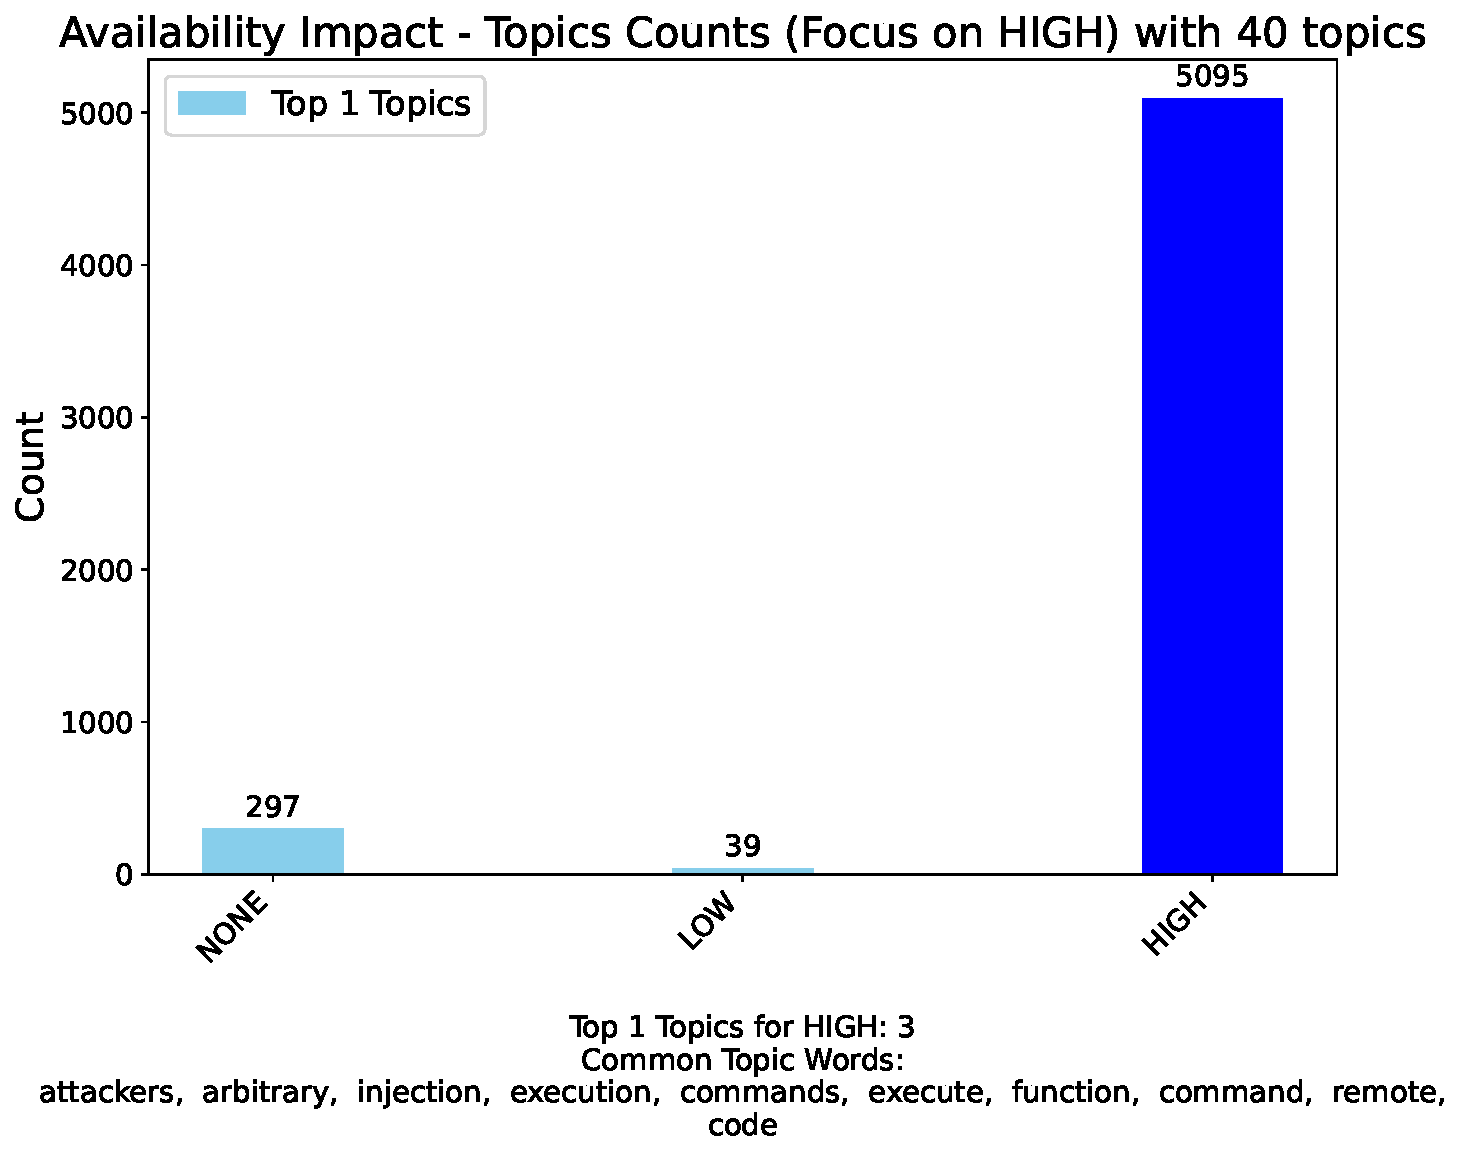
\includegraphics[width=0.7\textwidth]{figures/availabilityImpact/merged_top_k_topics_category_focus_counts_availabilityImpact_HIGH_k1.pdf}
		\caption{The counts of the documents within the best topic in relation to availabilityImpact
			with target class \texttt{HIGH}. Extra example showing that the best topic for
			availabilityImpact can include the expected denial of service related keywords}
		\label{fig:availabilityImpact_60_HIGH_denial}
	\end{subfigure}

\end{figure}
\subsubsection{Availability Impact: Focus on class NONE}

Figure \ref{fig:availabilityImpact_60_NONE} shows the distribution for the cluster best representing
the \texttt{NONE} class of availability impact.

Interestingly, this cluster primarily contains vulnerabilities related to web application security
issues, particularly injection attacks and cross-site scripting. While these vulnerabilities can be
severe in terms of confidentiality and integrity, they typically do not directly impact system
availability.

Key findings:

\begin{itemize}

	\item The cluster shows a clear majority of \texttt{NONE}-rated vulnerabilities for availability
	      impact.

	\item Predominant terms include \say{inject}, \say{arbitrary}, \say{html}, \say{cross}, \say{scripting}, \say{site},
	      \say{xss}, \say{user}, \say{stored}, and \say{web}.

	\item The presence of web application security terms suggests that these vulnerabilities, while
	      potentially severe in other aspects, do not typically cause system downtime or service
	      interruptions.

	\item This cluster effectively identifies vulnerabilities that, despite their severity in other
	      areas, have minimal impact on system availability.

\end{itemize}

\subsubsection{Availability Impact: Focus on class LOW}

Figure \ref{fig:availabilityImpact_60_LOW} represents the distribution for the cluster best
representing the \texttt{LOW} class of availability impact. However, this class requires
careful interpretation due to significant class imbalance in the dataset.

As evident from Figure \ref{fig:nvd_data}, the \texttt{LOW} class for Availability Impact is
highly under-represented in the true class values. This imbalance has a profound effect on our
clustering results, leading to a diluted cluster where the primary focus class is actually
\texttt{NONE} rather than \texttt{LOW}.

Key findings:

\begin{itemize}

	\item The cluster shows a majority of \texttt{NONE}-rated vulnerabilities, contrary to what we
	      would expect for a \texttt{LOW} class cluster.

	\item Predominant terms include \say{compromise}, \say{oracle}, \say{access}, \say{data}, \say{cvss}, \say{attacks},
	      \say{unauthorized}, \say{successful}, \say{accessible}, and \say{base}.

	\item The mix of terms suggests a broad range of vulnerabilities, many of which may not
	      significantly impact system availability.

	\item This cluster highlights the challenges in accurately identifying and categorizing
	      low-impact availability vulnerabilities due to their scarcity in the dataset.

\end{itemize}

The results for this class underscore a crucial limitation in our current model and dataset. The
severe underrepresentation of \texttt{LOW} Availability Impact vulnerabilities makes it difficult
for the model to accurately capture the characteristics of this class. Instead, the cluster is
dominated by \texttt{NONE} impact vulnerabilities, which are much more prevalent in the dataset.

This observation points to the need for careful consideration when interpreting results for
underrepresented classes in imbalanced datasets. It also suggests potential areas for improvement in
our model, such as employing techniques to address class imbalance or collecting more data for
underrepresented categories.

\subsubsection{Availability Impact: Focus on class HIGH}

Figure \ref{fig:availabilityImpact_60_HIGH} shows the distribution for the cluster best representing

the \texttt{HIGH} class of availability impact.

In this cluster, we see a clear focus on remote code execution and command injection
vulnerabilities. These types of attacks have the potential to severely compromise system
availability by allowing attackers to execute arbitrary code or commands, potentially leading to
system crashes or complete takeover.

Key findings:

\begin{itemize}

	\item The cluster shows a strong representation of \texttt{HIGH}-rated vulnerabilities for
	      availability impact.

	\item Predominant terms include \say{attackers}, \say{arbitrary}, \say{injection},
	      \say{execution}, \say{commands},
	      \say{execute}, \say{function}, \say{command}, \say{remote}, and \say{code}.

	\item The presence of terms like \say{remote} and \say{arbitrary} coupled with \say{execution} and \say{command}
	      suggests vulnerabilities that allow attackers to run malicious code, potentially causing
	      severe system disruptions.

	\item This cluster effectively captures severe availability threats that align with
	      cybersecurity expert expectations for high-impact availability issues.

\end{itemize}

The analysis of these clusters for Availability Impact reveals interesting distinctions between the
NONE, LOW, and HIGH categories. Notably, vulnerabilities that severely impact confidentiality or
integrity (such as XSS) are often categorized as having no availability impact. In contrast,
vulnerabilities allowing remote code execution or command injection are correctly identified as
high-impact for availability. This demonstrates the model's ability to differentiate between various
security impacts and accurately categorize vulnerabilities based on their potential to disrupt
system availability.


\subsection{Discussion of CVSS Impact Metrics}

Our analysis of the three CVSS impact metrics - Integrity, Confidentiality, and Availability -
reveals intriguing patterns and distinctions in how different types of vulnerabilities are
categorized. However, it's crucial to note the significant data imbalance in the Availability Impact
metric, which influences our interpretations and comparisons.

\subsubsection{Cross-Metric Comparisons}

\begin{itemize}

	\item \textbf{Web Application Vulnerabilities:} Cross-site scripting (XSS) and related web
	      vulnerabilities consistently appear in the LOW categories for both Integrity and
	      Confidentiality impacts. For Availability, these vulnerabilities predominantly fall into the
	      NONE class. This pattern underscores the nature of XSS attacks, primarily affecting data
	      integrity and confidentiality at the client-side but rarely causing system-wide availability
	      issues.

	\item \textbf{Remote Code Execution:} Vulnerabilities allowing remote code execution or
	      arbitrary command injection are categorized as HIGH impact across all three metrics. This
	      consistency emphasizes the severe and multi-faceted threat posed by such vulnerabilities.

	\item \textbf{Denial of Service:} Terms related to denial of service (DoS) attacks are prominent
	      in the NONE class for both Integrity and Confidentiality impacts. Denial of service and
	      related terms are sometimes absent from the Availability impact categories, particularly in
	      the HIGH class where we might expect them, this suggests some instability in this model
	      due to the imbalanced data.

\end{itemize}

\subsubsection{Metric-Specific Observations}

\begin{itemize}

	\item \textbf{Integrity Impact:} The progression from NONE to HIGH in Integrity Impact shows a
	      clear escalation from system crashes to XSS to remote code execution, aligning well with
	      expected severity levels for integrity breaches.

	\item \textbf{Confidentiality Impact:} The Confidentiality metric effectively differentiates
	      between vulnerabilities affecting individual user data (LOW impact, often web-related) and
	      those exposing system-wide information (HIGH impact, often involving remote access).

	\item \textbf{Availability Impact:} The severe underrepresentation of LOW Availability Impact
	      vulnerabilities significantly affects our analysis. The NONE and HIGH categories are more
	      reliably represented, showing a distinction between vulnerabilities that don't typically
	      affect system uptime (web vulnerabilities in NONE class) and those that could lead to
	      system-wide disruptions (remote code execution in HIGH class). However, the lack of a
	      well-defined LOW class limits our ability to observe a clear progression of severity in
	      this metric.

\end{itemize}

\subsubsection{Implications for Vulnerability Assessment}

\begin{itemize}

	\item \textbf{Contextual Importance:} Our analysis reinforces the importance of context in
	      vulnerability assessment. The same vulnerability type can have varying impacts across
	      different security aspects, emphasizing the need for a multi-dimensional approach to
	      security scoring.

	\item \textbf{Data Imbalance Considerations:} The Availability Impact metric highlights the
	      challenges posed by imbalanced datasets in vulnerability classification. This imbalance
	      affects our model's ability to accurately categorize and interpret LOW impact availability
	      vulnerabilities, underscoring the need for careful data curation and potentially specialized
	      modeling techniques for underrepresented classes.

	\item \textbf{Severity Nuances:} Where data is sufficiently representative, our clustering
	      results capture nuances in severity levels effectively. The distinction between LOW and HIGH
	      impacts often lies in the scope of the vulnerability - whether it affects individual
	      sessions or has system-wide implications.

	\item \textbf{Alignment with Expert Knowledge:} For well-represented categories, the topic
	      distributions largely align with cybersecurity expert expectations. However, the data
	      imbalance in Availability Impact suggests that our model may not fully capture the nuances
	      experts consider for this metric, particularly for low-impact availability issues.

\end{itemize}

\subsection{Cluster Merging and Refinement}

In an attempt to enhance class representation and potentially improve the overall performance of the
topic model, I explored the concept of merging related clusters. This process involved several steps:

\begin{itemize}

	\item Identifying clusters with overlapping representation of CVSS classes.

	\item Merging these clusters by combining their topic-word distributions and reassigning documents.

	\item Recalculating class representation metrics for the merged clusters.

	\item Comparing the performance of the merged model to the original in terms of:

	      \begin{itemize}

		      \item Clarity of class representation

		      \item Interpretability of resulting topics

	      \end{itemize}

\end{itemize}

\subsubsection{Methodology}

Clusters were merged by finding the top-k best clusters in the cluster distribution. While this
method is straightforward to implement, it is admittedly crude and may not capture all the nuances
of semantic similarity between topics.

Other approaches exist, for instance, Neuhaus \& Zimmerman
(2010)~\cite{cve_topic_modelling} merged clusters based on the similarity of the topic words found
by their model. This other approach potentially offers a more nuanced way of identifying truly related topics.

\subsubsection{Results}

To illustrate the effects of cluster merging, we present the following Figures~\ref{fig:integrityImpact_60_NONE_merged},~\ref{fig:confidentialityImpact_60_LOW_merged}

\begin{figure}[h!]
	\ContinuedFloat*
	\centering
	\begin{subfigure}{\textwidth}
		\centering
		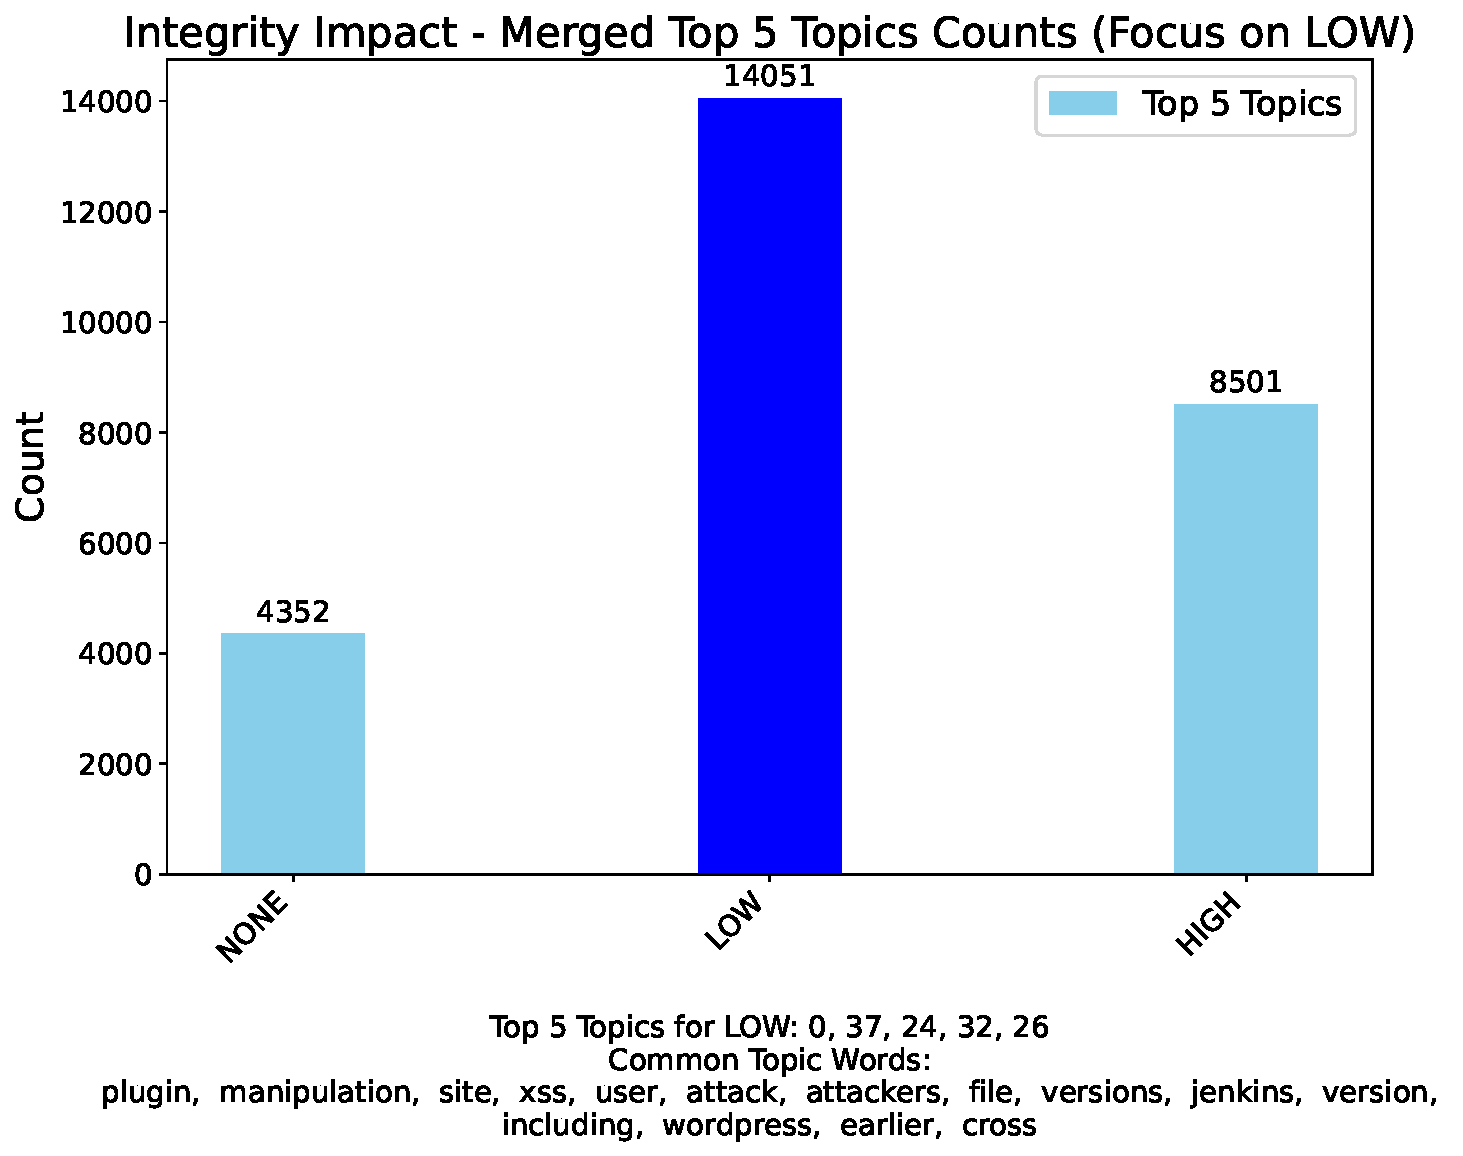
\includegraphics[width=0.7\textwidth]{figures/integrityImpact/merged_top_k_topics_category_focus_counts_integrityImpact_LOW_k5.pdf}
		\caption{The counts of the documents within the best five topics merged in relation to \texttt{Integrity
				Impact} with
			target class \texttt{LOW}}

		\label{fig:integrityImpact_60_NONE_merged}
	\end{subfigure}
	\caption{Counts of Merged Topic Clusters}

\end{figure}

\begin{figure}[h!]
	\ContinuedFloat
	\centering
	\begin{subfigure}{\textwidth}
		\centering
		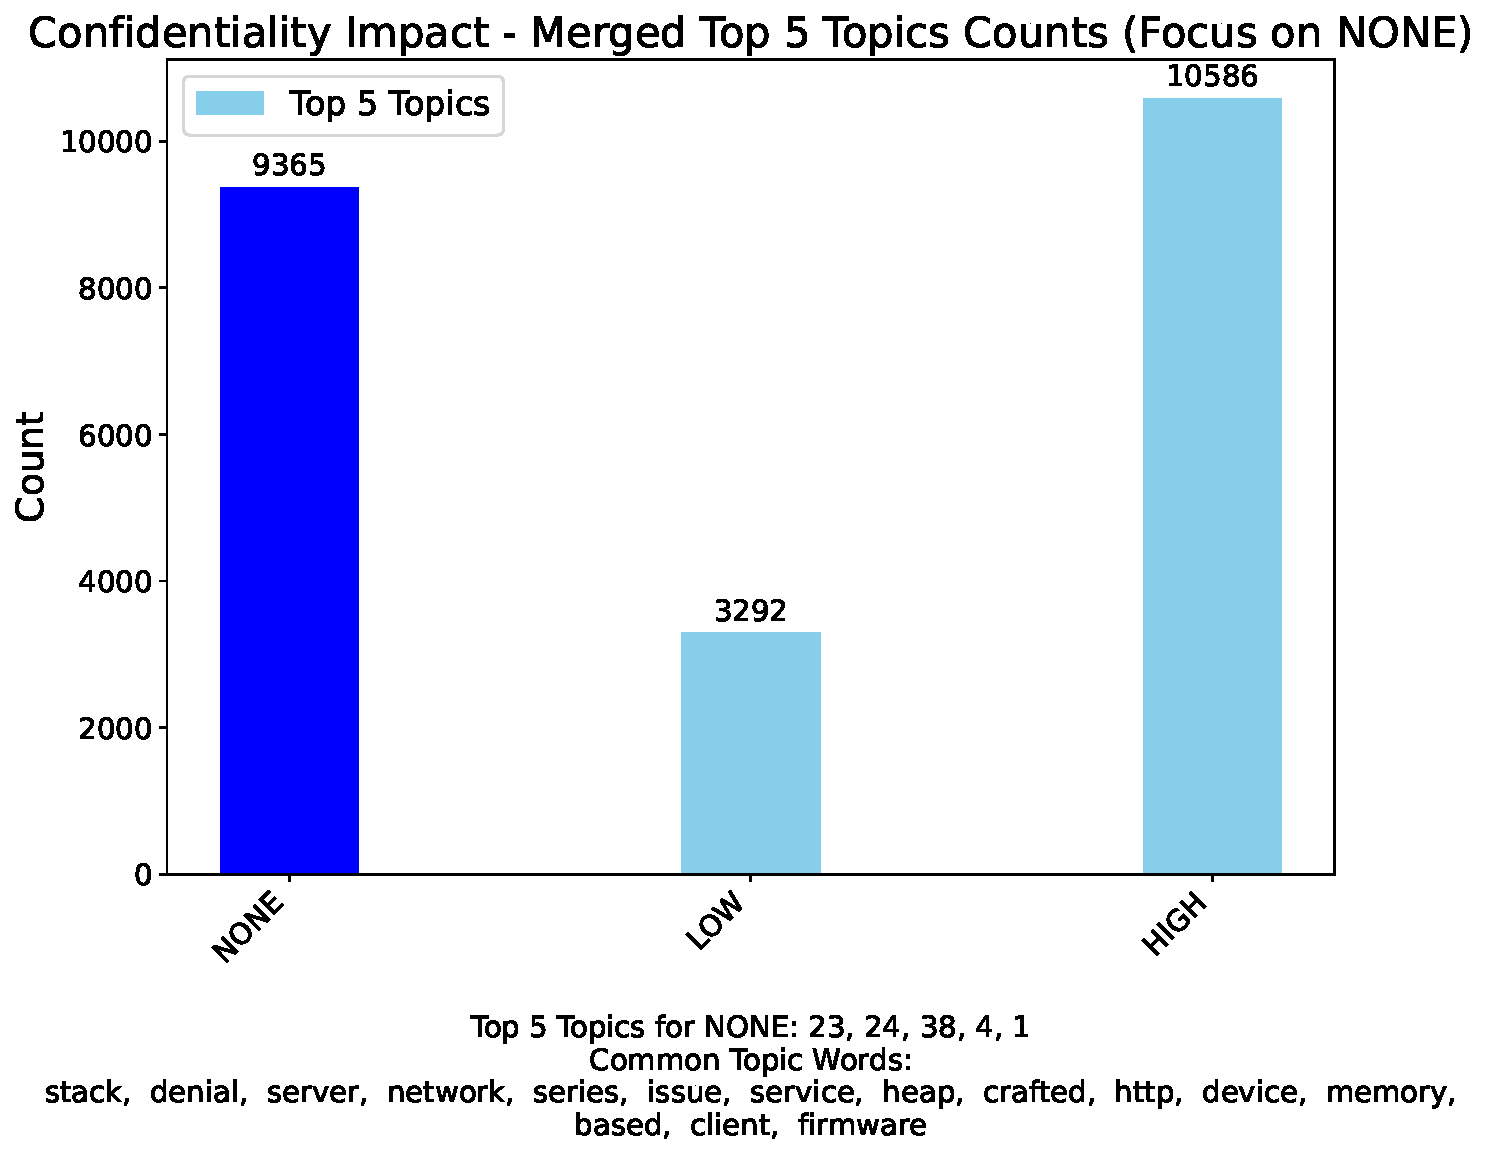
\includegraphics[width=0.7\textwidth]{figures/confidentialityImpact/merged_top_k_topics_category_focus_counts_confidentialityImpact_NONE_k5.pdf}
		\caption{The counts of the documents within the best topic in relation to \texttt{Integrity Impact} with target class \texttt{LOW}}
		\label{fig:confidentialityImpact_60_LOW_merged}
	\end{subfigure}

	\caption{Counts of Merged Topic Clusters}
\end{figure}

Contrary to our initial expectations, the process of merging clusters did not lead to improved
results. Instead, I observed the following effects:

The merging of clusters resulted in several negative impacts on the model's quality and utility. The
process led to decreased cluster purity, with a higher mix of different CVSS classes within each
cluster. This reduction in homogeneity made the larger, merged clusters more difficult to interpret,
diluting their defining characteristics and semantic meanings. Consequently, the model lost
granularity, as specific types of vulnerabilities or attack vectors were grouped into broader, less
nuanced categories. Overall, these changes contributed to a decrease in topic coherence, indicating
that the merged clusters were less internally consistent than their more granular predecessors.


\subsection{Interpretation and Future Directions}

These results suggest that our initial clustering approach was already capturing meaningful
distinctions between different types of vulnerabilities and their associated CVSS ratings. The
process of merging clusters, at least with the current methodology, appears to obscure these
distinctions rather than enhance them.

However, this does not necessarily mean that cluster merging is inherently unhelpful. Instead, it
suggests that more sophisticated merging strategies may be needed to preserve the valuable
information captured in the original clusters while still allowing for the combination of truly
related topics.

\subsection{Overall Observations}

\begin{enumerate}

	\item Our clustering approach successfully differentiated between vulnerabilities with varying
	      levels of integrity impact, as evidenced by the distinct profiles of each cluster.

	\item The results align well with expert knowledge in the field of cybersecurity, suggesting
	      that our unsupervised learning approach can capture meaningful patterns in vulnerability
	      data.

	\item While our current analysis provides a static view of the vulnerability landscape, the
	      temporal aspect of the data presents an opportunity for future research. Analyzing how these
	      clusters and trends have evolved over time could provide additional insights into the
	      changing nature of cybersecurity threats.

	\item The overlap between categories in some clusters (particularly visible in the \texttt{LOW}
	      class) highlights the complexity of vulnerability classification and the potential for
	      ambiguity in CVSS scoring.

\end{enumerate}


\subsection{Future Work}

As I am a Masters student, I will be continuing the work that I have done here for COSC480 into next
year. My future work will focus on several key areas:

\begin{itemize}

	\item \textbf{Dataset Refinement:} The CVE dataset contains numerous poorly written descriptions
	      that hinder machine learning model performance. We plan to develop robust methods for
	      identifying and filtering out low-quality entries, potentially using the insights gained
	      from our clustering analysis.

	\item \textbf{Advanced Clustering Techniques:} Building on our current work, we aim to explore
	      more sophisticated clustering approaches. This includes implementing the cluster merging
	      method proposed by Neuhaus \& Zimmerman (2010)~\cite{cve_topic_modelling}, which focuses on
	      the similarity of topic words.

	\item \textbf{Temporal Analysis:} We intend to investigate how vulnerability patterns and their
	      CVSS ratings evolve over time. This could involve applying dynamic topic modeling techniques
	      to capture temporal trends in the data.

\end{itemize}

Through these efforts, I aim to develop a more robust, data-driven approach to vulnerability
analysis and CVSS scoring that can adapt to the evolving landscape of cybersecurity threats.

\section{Conclusion}

The Common Vulnerability Scoring System (CVSS) plays a vital role in prioritizing and managing the
ever-increasing number of software vulnerabilities. This research has highlighted both the strengths
and limitations of current CVSS implementation and scoring practices.

Key findings from our study include:

\begin{itemize}

	\item \textbf{Database Variability:} We observed variability in CVSS scores between
	      different databases, such as NVD and MITRE. This inconsistency underscores the subjective
	      nature of vulnerability scoring and the challenges in establishing a reliable ground truth.

	\item \textbf{Clustering Insights:} The application of Latent Dirichlet Allocation (LDA) for
	      clustering CVE descriptions revealed meaningful patterns in vulnerability types and their
	      associated CVSS ratings. This demonstrates the potential of unsupervised learning techniques
	      in capturing latent structures within vulnerability data.

	\item \textbf{Cluster Merging Limitations:} Our experiments with cluster merging, while not
	      yielding immediate improvements, provided valuable insights into the robustness of our
	      initial clustering and the complexity of semantic relationships between vulnerability types.

	\item \textbf{Data Quality Importance:} The analysis highlighted the critical role of data
	      quality in both manual and automated CVSS scoring processes. Poorly written or inconsistent
	      CVE descriptions pose significant challenges for accurate vulnerability assessment.

\end{itemize}

While CVSS remains a crucial tool for vulnerability management, our research suggests that its
current implementation has limitations that need to be addressed. The integration of machine
learning models, particularly those focused on natural language processing and topic modeling,
offers promising avenues for automating and enhancing the accuracy of CVSS scoring.

By combining advanced machine learning techniques with domain expertise in cybersecurity, we can
work towards a more consistent, accurate, and interpretable system for assessing and prioritizing
software vulnerabilities. This improved system would not only enhance the efficiency of
vulnerability management but also contribute to a more secure digital ecosystem overall.


\printbibliography[title={References}]



\appendix

\renewcommand{\thesection}{Appendix \Alph{section}}

\subsection{CVSS figures from other versions}

Below is a collection of confusion matrics which are results from the Bayesian analysis of CVSS
versions 2.0 \& 3.0 for both the NVD and MITRE databases. Version 2.0 for MITRE is especially rough
as there was very little data.

\begin{figure}[H]
	\centering
	\makebox[\textwidth][c]{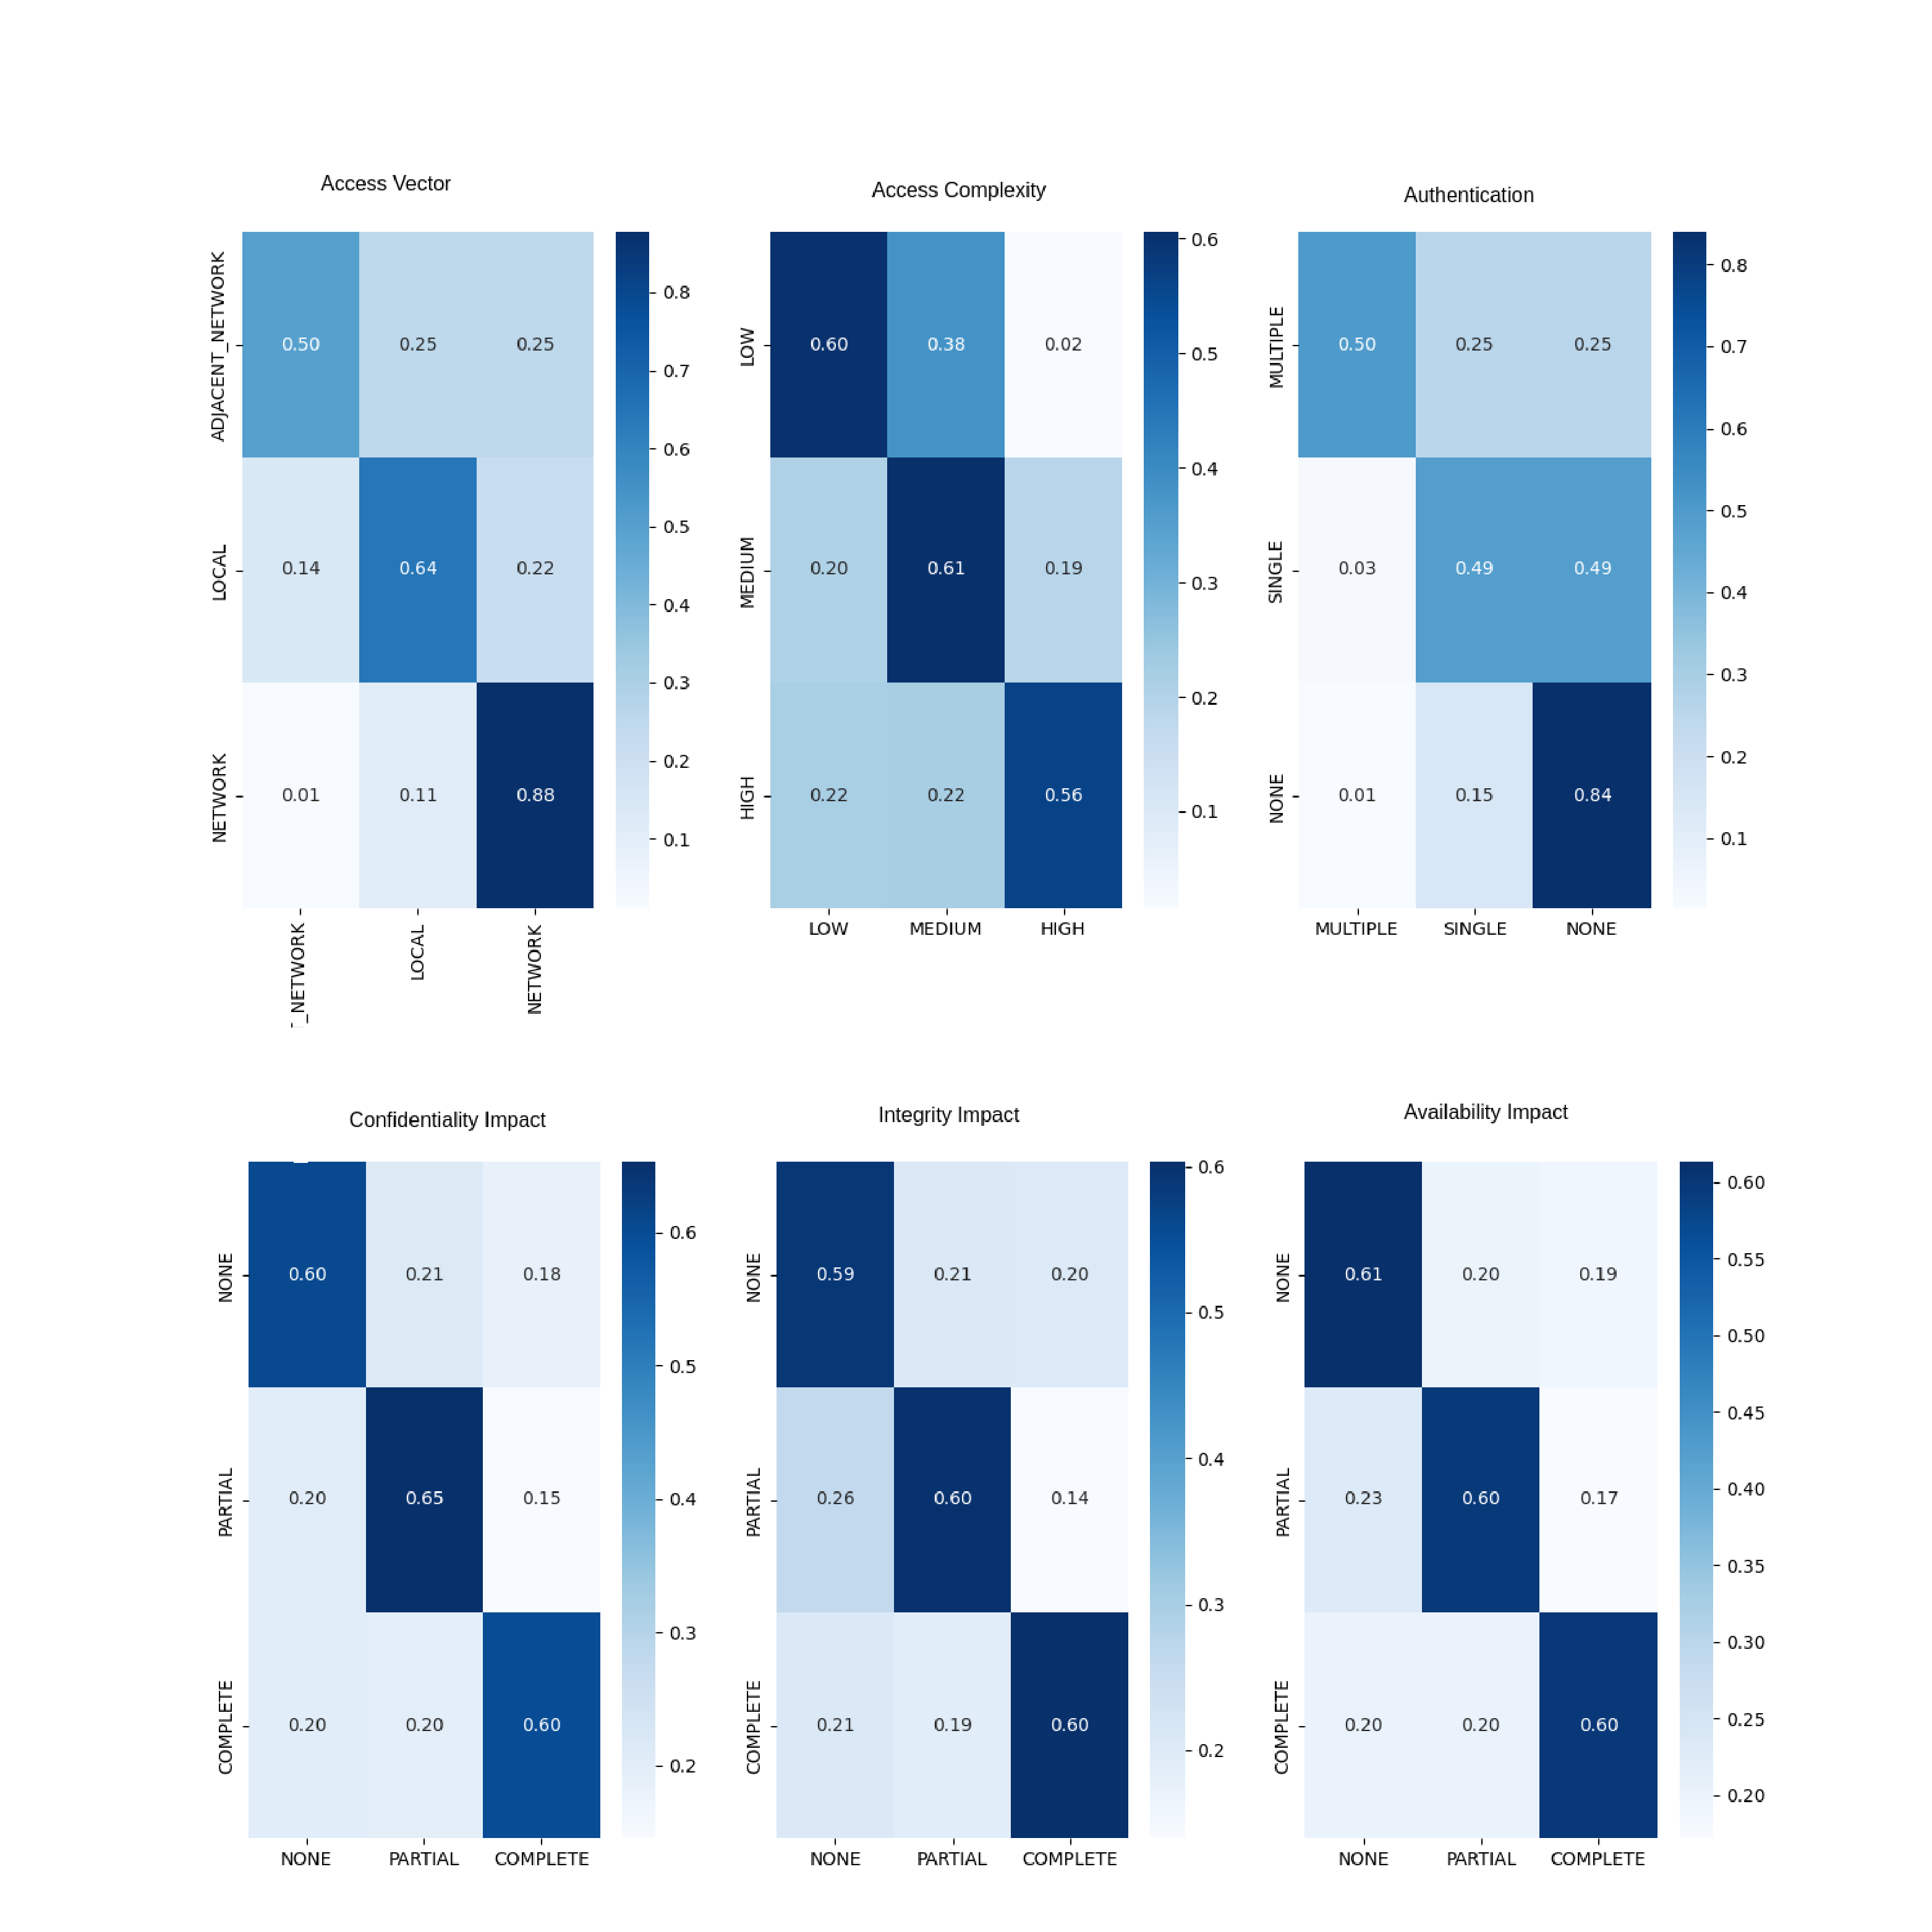
\includegraphics[width=1.5\textwidth]{{figures/nvd_2_titles.pdf}}}%
	\caption{\label{fig:nvd_2_confusion_matrices}Confusion matrix of estimated accuracy for CVSS metrics for version 2.0 for NVD}
\end{figure}

\begin{figure}[H]
	\centering
	\makebox[\textwidth][c]{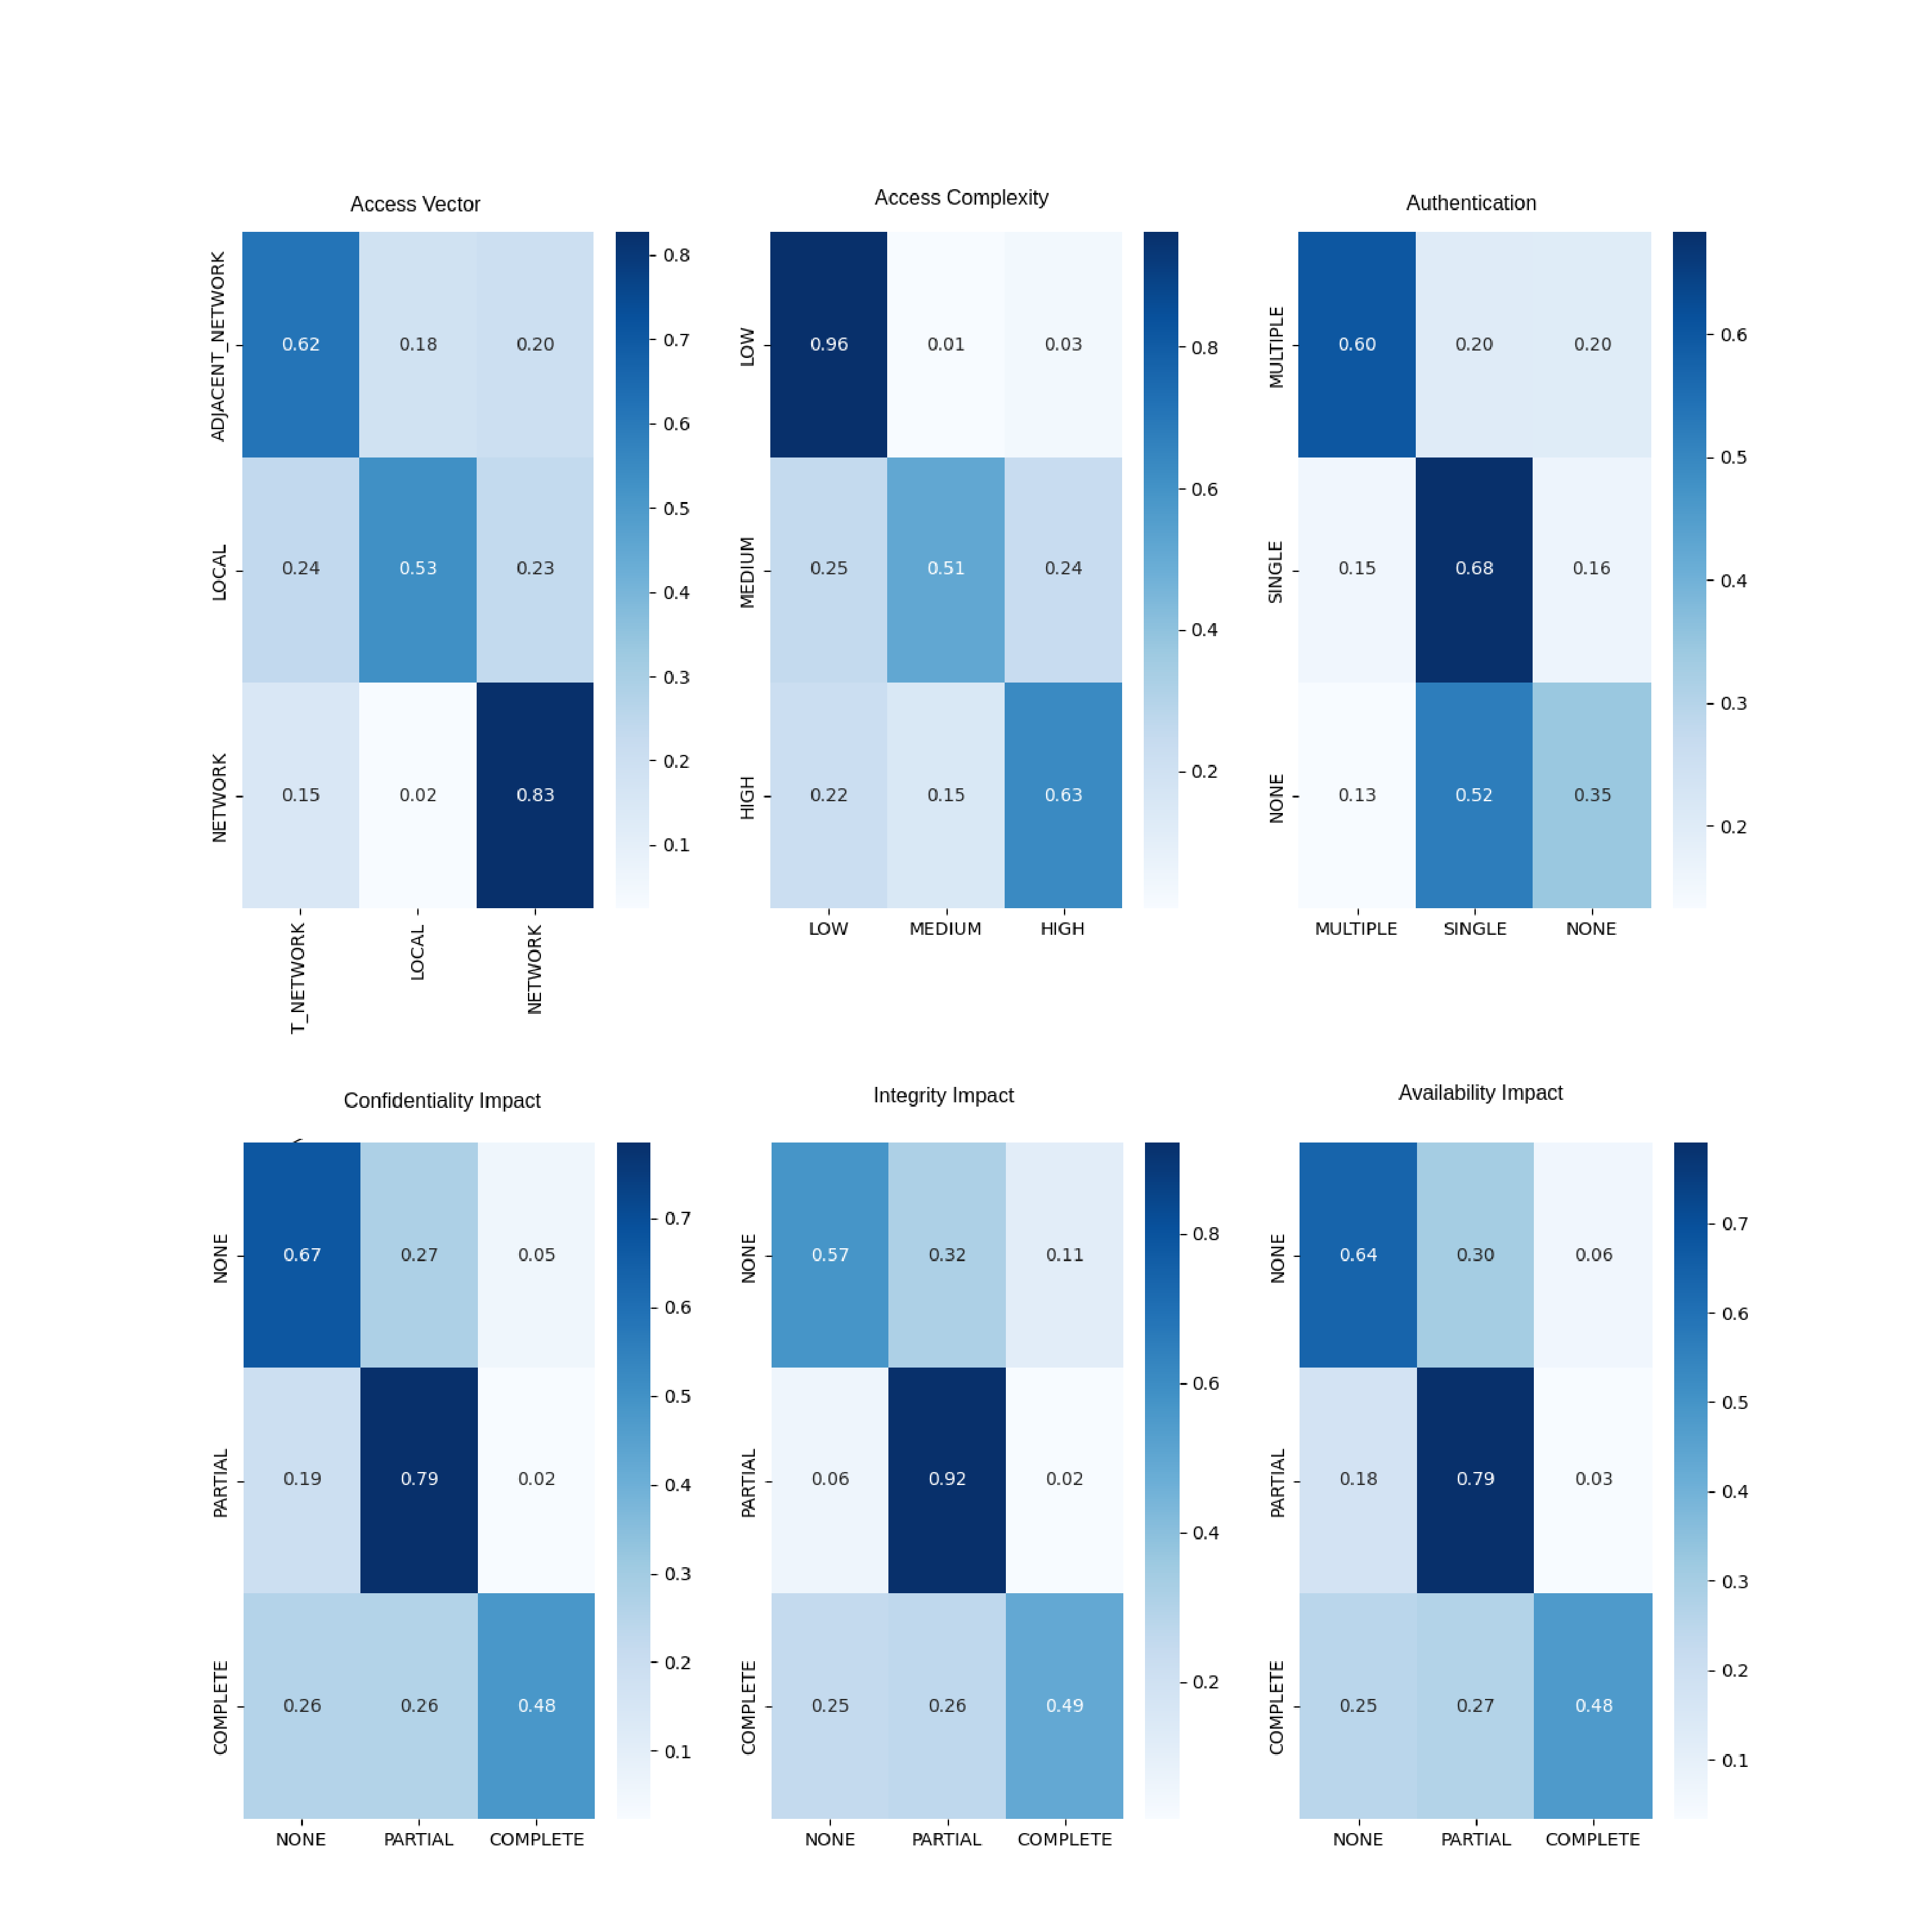
\includegraphics[width=1.5\textwidth]{figures/mitre_2_titles.pdf}}
	\caption{\label{fig:mitre_2_confusion_matrices}Confusion matrix of estimated accuracy for CVSS
		metrics for version 2.0 for MITRE}
\end{figure}

\begin{figure}[H]
	\centering
	\makebox[\textwidth][c]{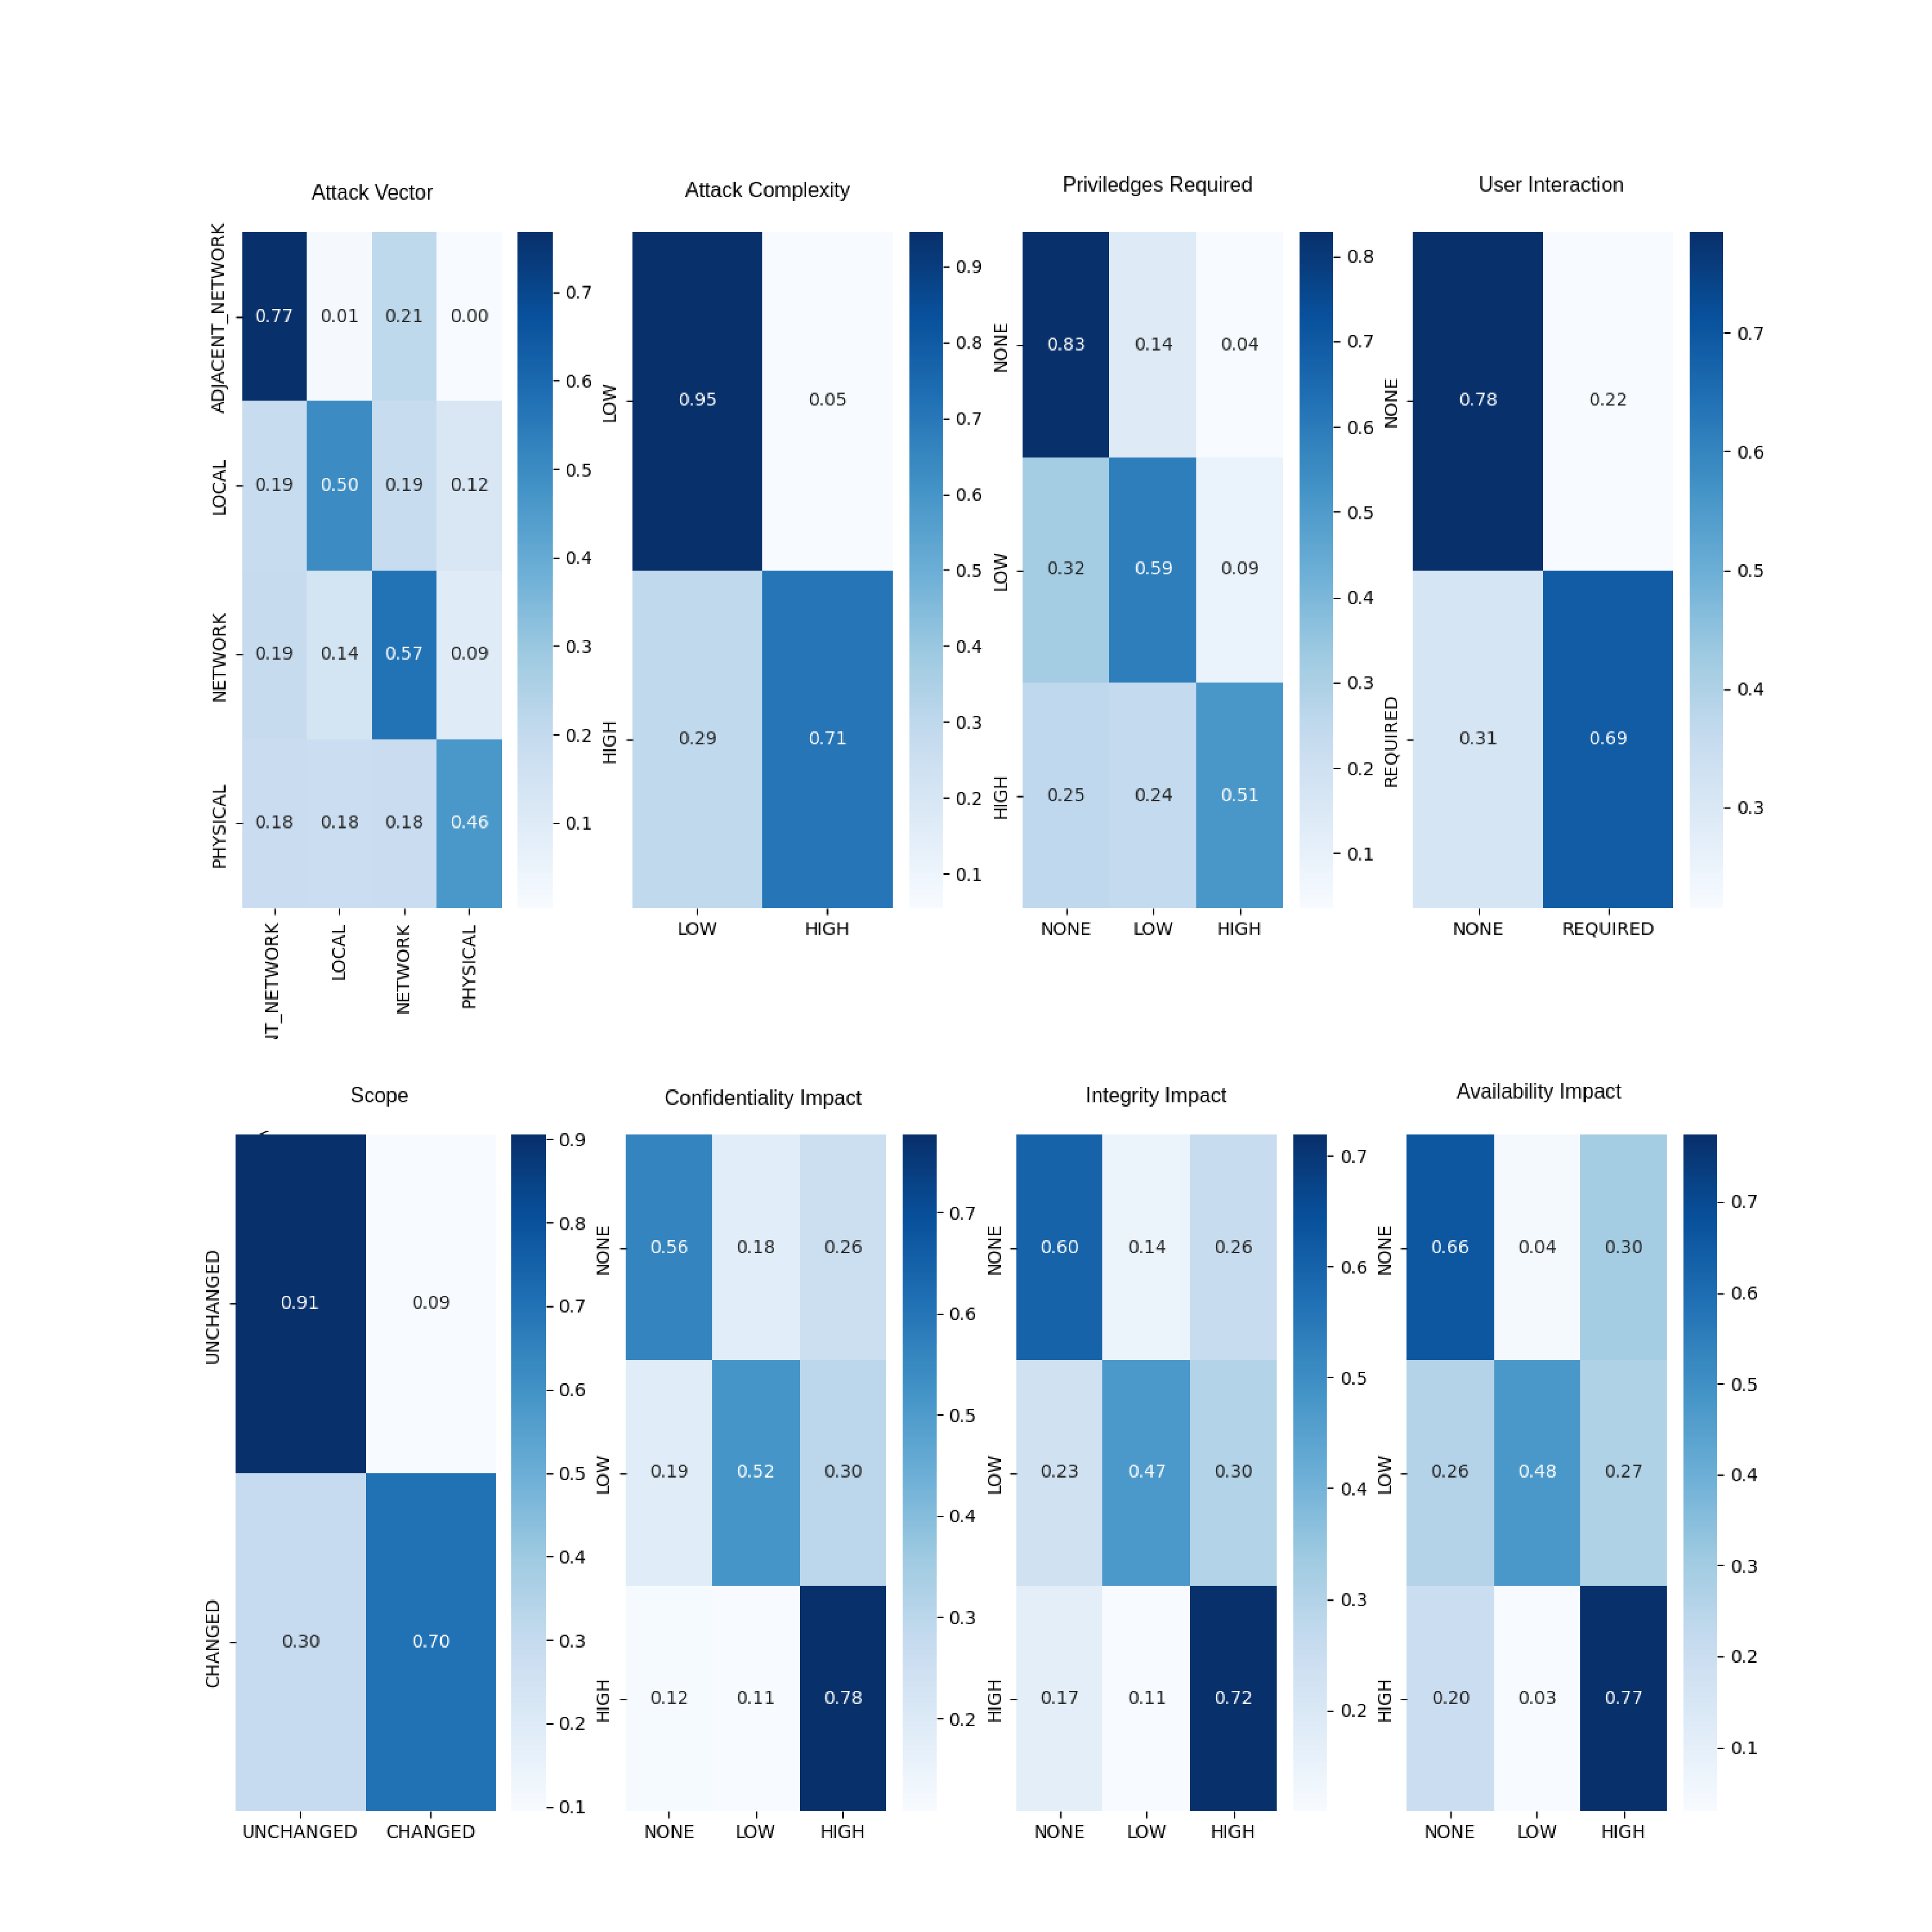
\includegraphics[width=1.5\textwidth]{figures/nvd_30_titles.pdf}}
	\caption{\label{fig:nvd_30_confusion_matrices}Confusion matrix of estimated accuracy for CVSS metrics for version 3.0 for NVD}
\end{figure}

\begin{figure}[H]
	\centering
	\makebox[\textwidth][c]{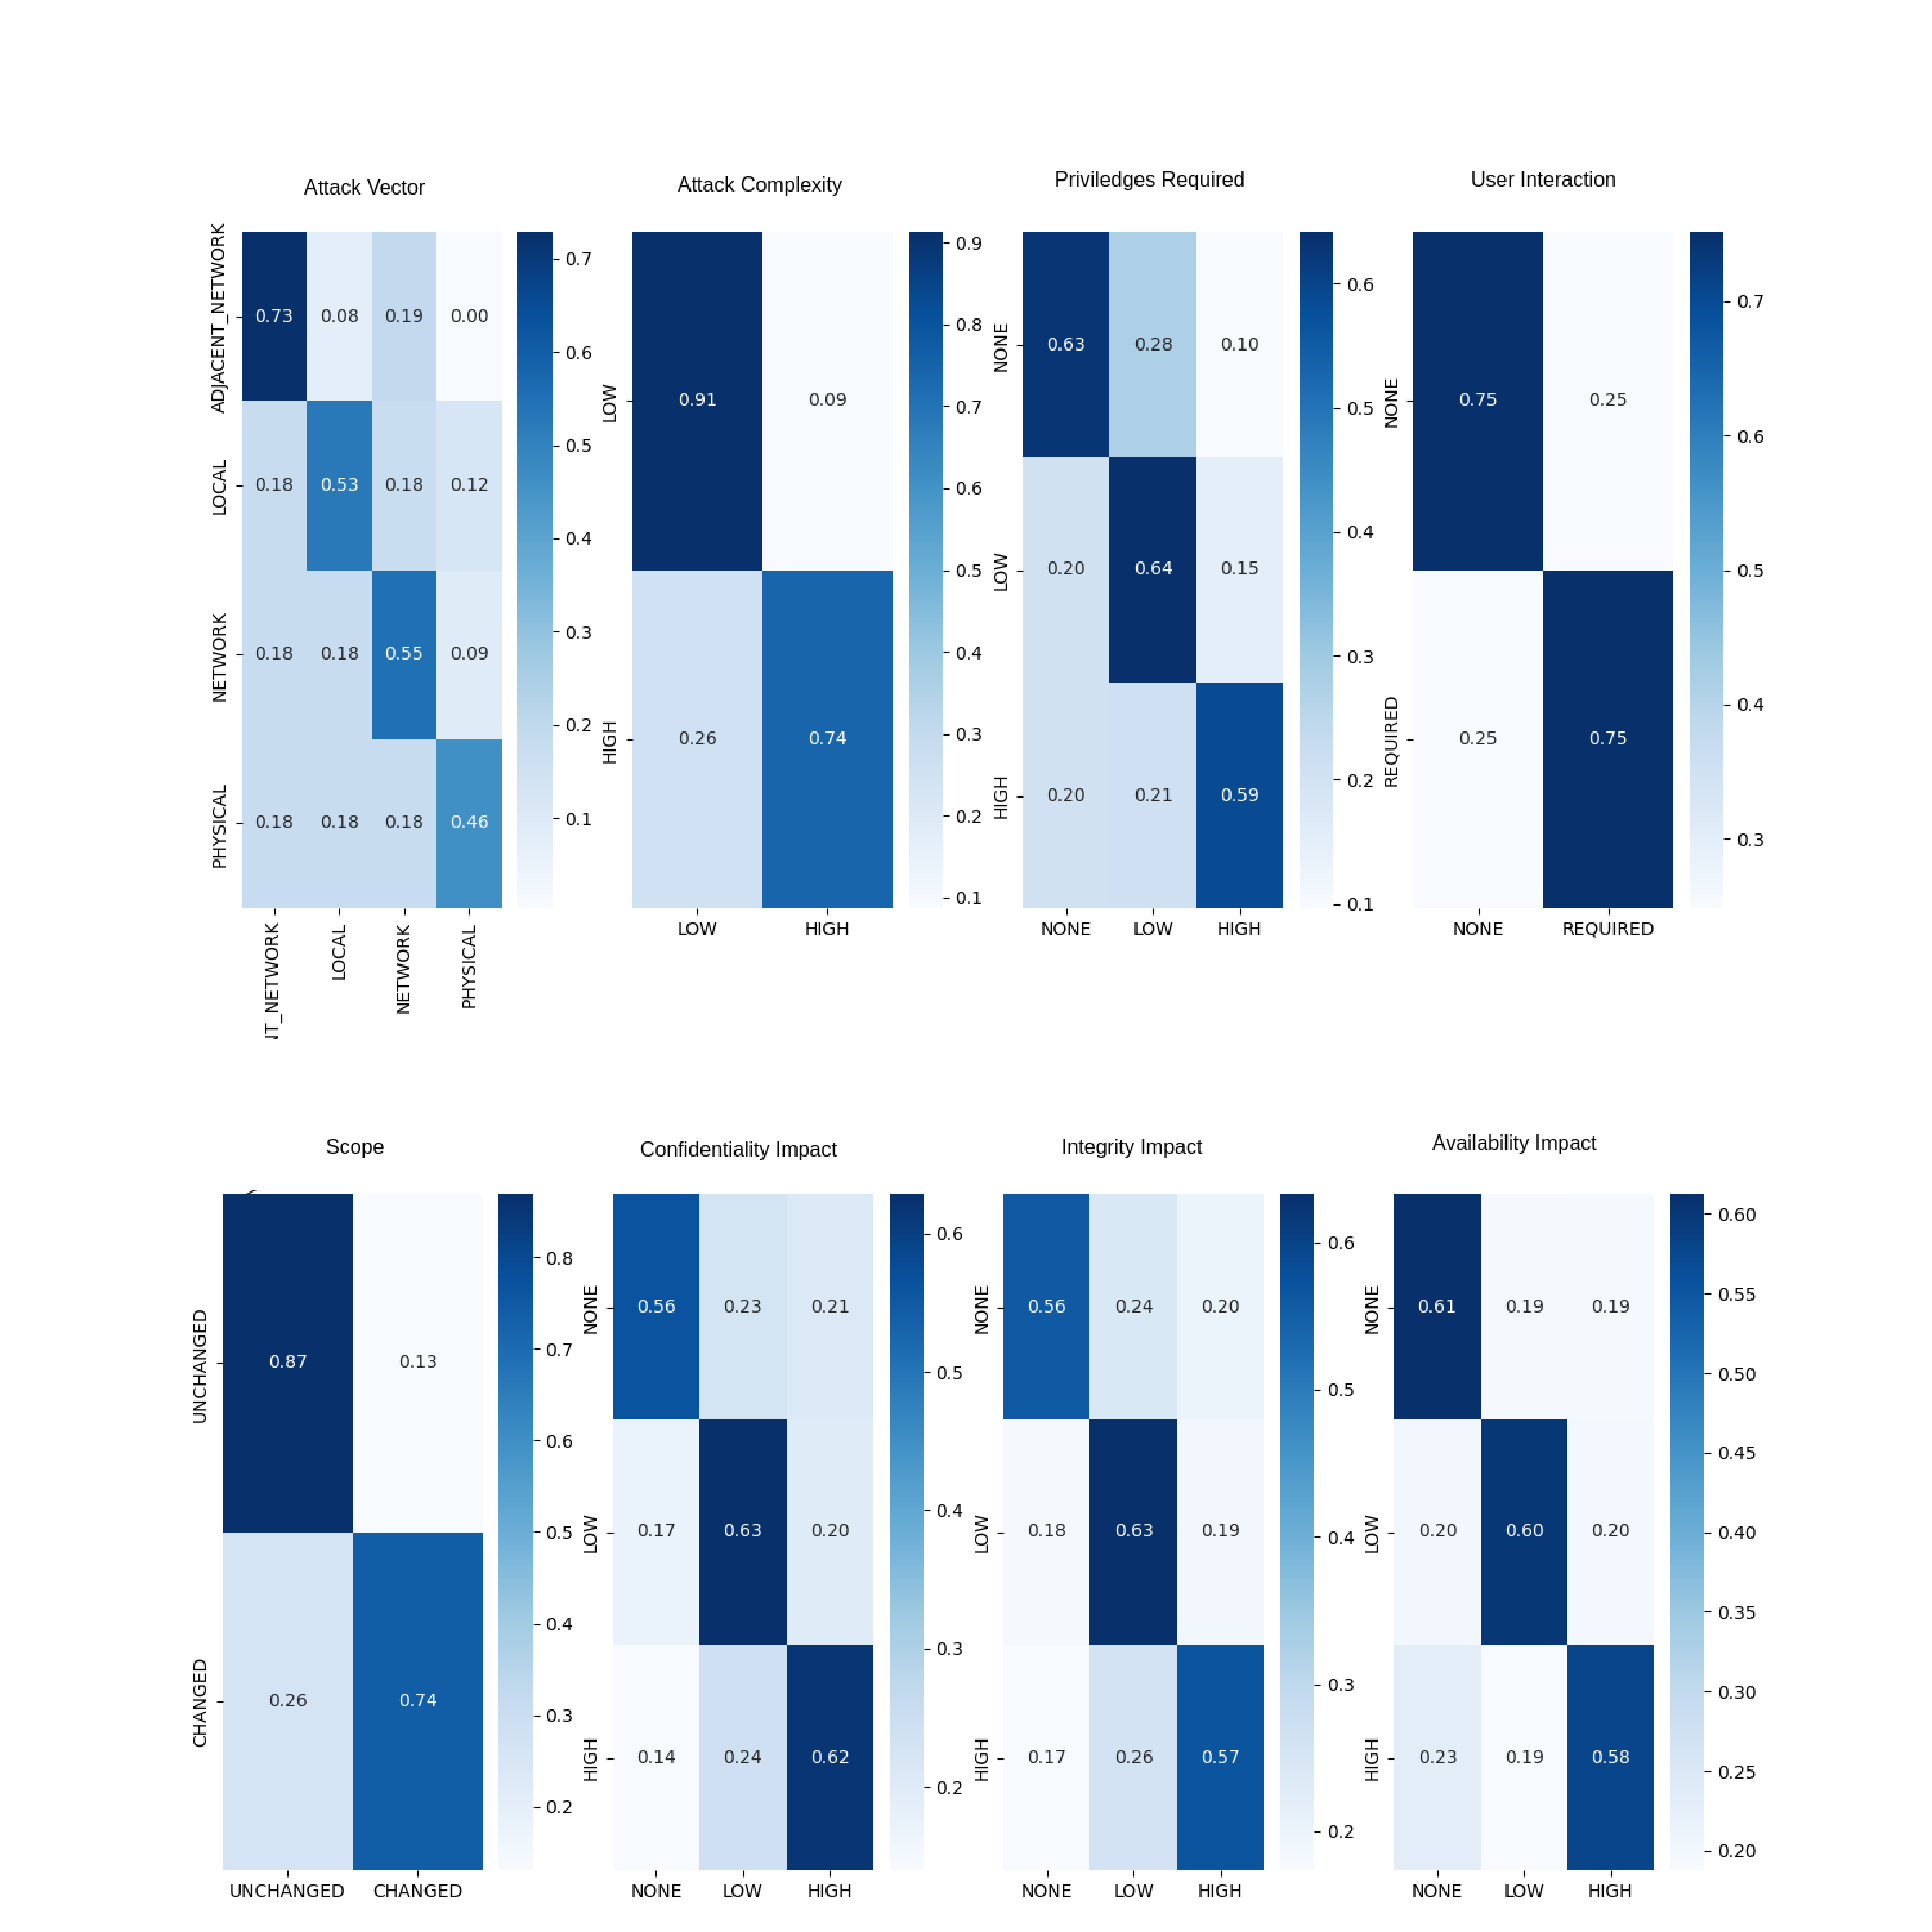
\includegraphics[width=1.5\textwidth]{figures/mitre_30_titles.pdf}}
	\caption{\label{fig:mitre_30_confusion_matrices}Confusion matrix of estimated accuracy for CVSS
		metrics for version 3.0 for MITRE}
\end{figure}



\subsection{CVSS 3.1 Base Score formula} \label{equation}

Below is a formulaic representation of the CVSS 3.1 base score formula.
	{\scriptsize
		\begin{equation}
			ISS = 1 - ((1 - Confidentiality) \times (1 - Integrity) \times (1 - Availability)) \\
		\end{equation}
		\begin{equation}
			Impact =
			\begin{cases}
				7.52 \times (ISS - 0.029) - 3.25 \times (ISS - 0.02)^{15} & \text{if \textit{Scope} is
				\textit{Changed}}                                                                      \\
				6.42 \times ISS                                           & \text{if \textit{Scope} is
					\textit{Unchanged}}
			\end{cases}
		\end{equation}

		\begin{equation}
			Exploitability = 8.22 - AttackVector \times AttackComplexity \times PrivilegesRequired \times
			UserInteraction \\
		\end{equation}

		\begin{equation}
			Base Score =
			\begin{cases}
				0                                                           & Impact \leq 0              \\
				Roundup(Minimum(1.08 \times (Impact + Exploitability), 10)) & \text{if \textit{Scope} is
				\textit{Changed}}                                                                        \\
				Roundup(Minimum((Impact + Exploitability), 0))              & \text{if \textit{Scope} is
				\textit{Unchanged}}                                                                      \\
			\end{cases}
		\end{equation}
	}

\subsection{Exploit Prediction Scoring System diagrams for reference}

Below are two graphs from FIRST, the creator of EPSS. These show some of the results they have
found for this system, especially when comparing EPSS to CVSS in terms of effeciency of effort if
you use EPSS to guide remediation of vulnerabilities.

\begin{figure}
	\centering
	\makebox[\textwidth][c]{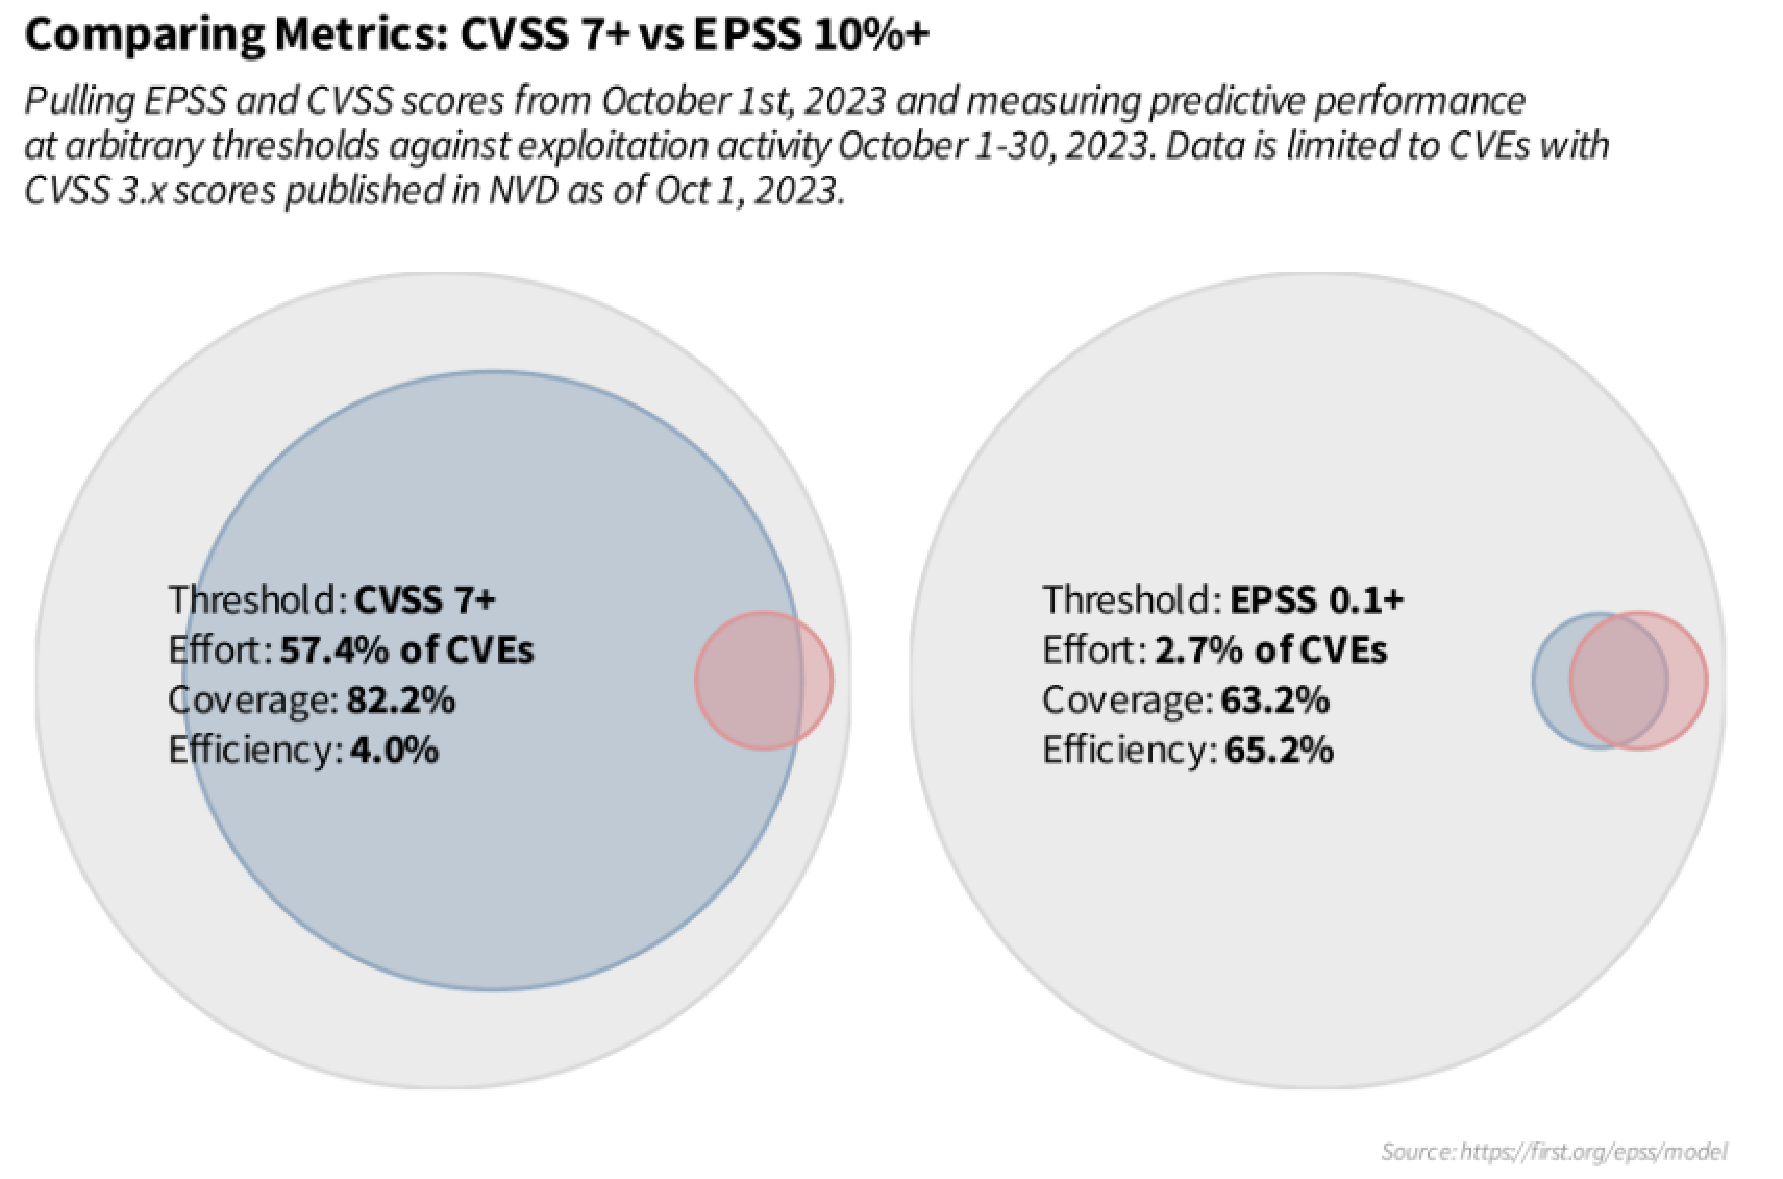
\includegraphics[width=1\textwidth]{figures/epss.pdf}}
	\caption{\label{fig:epss}Comparing Metrics: CVSS 7+ vs. EPSS 10\%+ sourced from \cite{EPSS}}
\end{figure}

\begin{figure}
	\centering
	\makebox[\textwidth][c]{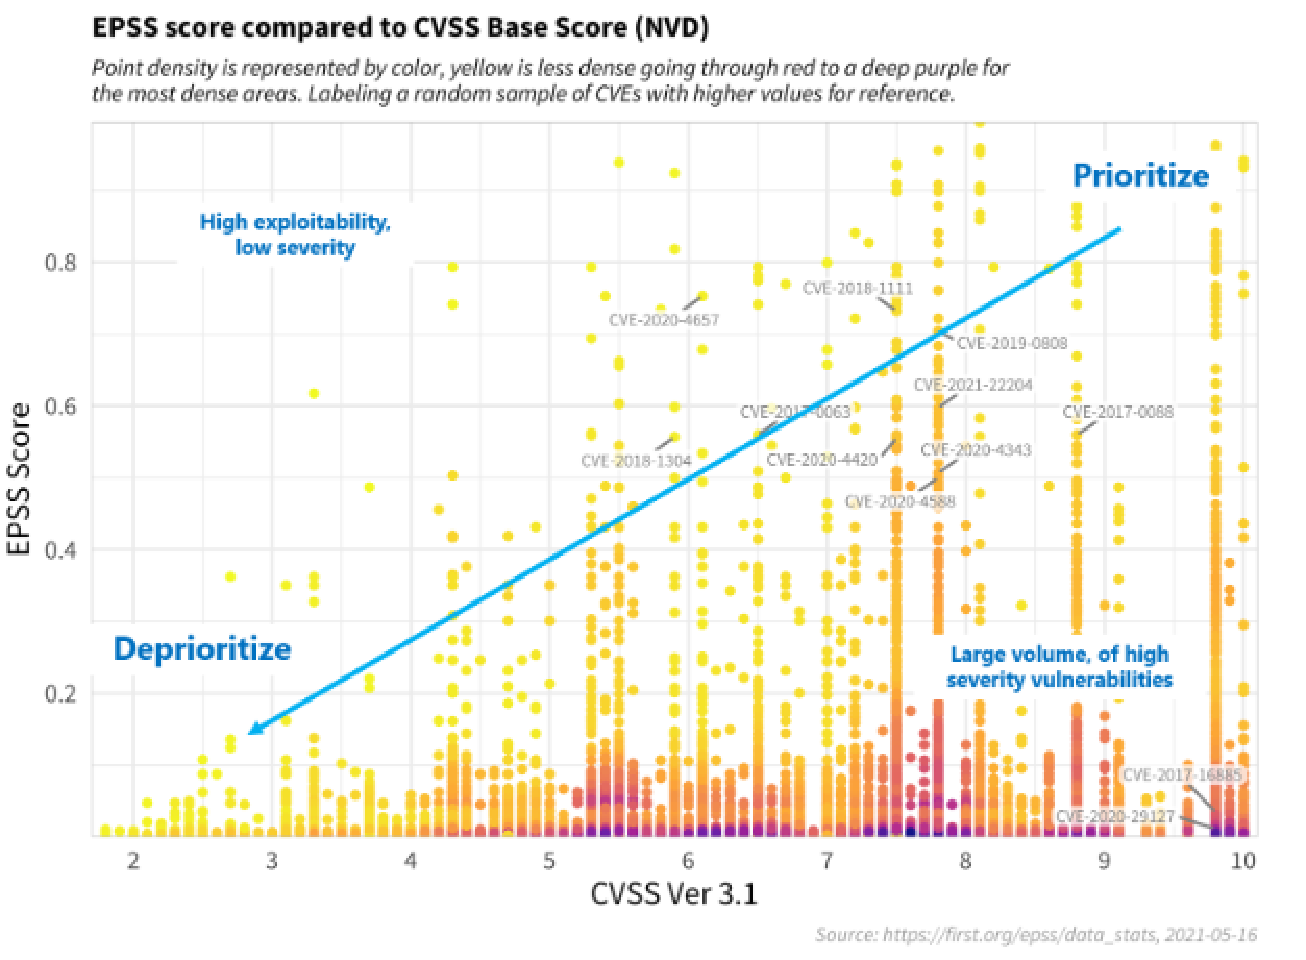
\includegraphics[width=1\textwidth]{figures/epss_and_cvss.pdf}}
	\caption{\label{fig:epss_and_cvss}EPSS score compared to CVSS Base Score (NVD) sourced from
		\cite{EPSS_USER}}
\end{figure}

\section{Aims and Objectives}

\subsection{Original}

\paragraph{Aims}
The primary aim of this research is to develop sophisticated predictive models capable of accurately determining
the severity levels of security threats based on the CVSS. This will involve a comprehensive review and comparison
of current datasets, with a focus on leveraging natural language descriptions provided in security vulnerability reports.
The project intends to utilize advanced transformer-based models to achieve this goal, contributing to the field of
cybersecurity by enhancing the precision of threat severity assessments.

\paragraph{Objectives}
\begin{itemize}[noitemsep]
	\item Conduct a comprehensive literature review to understand the current landscape of CVSS score prediction and the methodologies employed in existing models.
	\item Replicate successful methodologies to verify the accuracy of CVSS score databases, with a particular focus on alignment with recent CVSS standards and datasets.
	\item Explore opportunities for enhancing existing methodologies, including the investigation of data amalgamation from multiple databases to ascertain improvements in model performance.
	\item Experiment with various model architectures to identify the most effective approach in terms of predictive accuracy, specifically focusing on metrics such as the F1 score and balanced accuracy.
\end{itemize}

\paragraph{Timeline}
\begin{itemize}[noitemsep]
	\item March: Initiate the project with a literature review, system environment setup, and resource gathering.
	\item March-April: Replicate existing methodologies to validate findings and ensure alignment with current standards.
	\item May-June: Generate preliminary results and compile an interim report detailing findings and methodologies.
	\item July-August: Conduct experiments with various data source combinations and model architectures to identify optimal configurations.
	\item September-October: Finalize experimental work, analyze results, and prepare the comprehensive final report.
\end{itemize}

\subsection{Revised}

\paragraph{Aims}

The primary aim of this research is to develop sophisticated predictive models capable of accurately determining
the severity levels of security threats based on the CVSS. This will involve a comprehensive review and comparison
of current datasets, with a focus on leveraging natural language descriptions provided in security vulnerability reports.
The project intends to utilize advanced transformer-based models to achieve this goal, contributing to the field of
cybersecurity by enhancing the precision of threat severity assessments.

\paragraph{Objectives}
\begin{itemize}[noitemsep]

	\item Conduct a comprehensive literature review to understand the current landscape of CVSS
	      score prediction and the methodologies employed in existing models.

	\item Replicate successful methodologies to verify the accuracy of CVSS score databases, with a
	      particular focus on alignment with recent CVSS standards and datasets.

	\item Explore opportunities for enhancing existing methodologies, including the investigation of
	      data amalgamation from multiple databases to ascertain improvements in model performance.

	\item Look into data cleaning and clustering, to improve the efficacy of the models, as well as
	      a look into interpretability though data analysis.

\end{itemize}

\end{document}

